\documentclass[12pt, a4paper]{report}
\usepackage[utf8]{inputenc} % Cargar antes que babel si es necesario
\usepackage[spanish]{babel}
\usepackage{float}
\usepackage{amsmath}
\usepackage{multirow}
\usepackage{subcaption}
\usepackage{booktabs}
\usepackage{tabularx} 
\usepackage[numbers]{natbib}
\usepackage{enumitem}
\usepackage{graphicx} % Required for inserting images
\usepackage{times}
\usepackage[utf8]{inputenc}
\usepackage{geometry} %%%
\geometry{a4paper, left=22mm,  top=22mm, bottom=22mm, right=22mm}
% \usepackage{stringstrings}
% \usepackage{ifthen}
\usepackage{array}
\usepackage[intoc]{nomencl}
\usepackage{lipsum} % for template filler text

% \usepackage{setspace}
% \usepackage[document]{ragged2e}
\newcommand*\beginfrontmatter
    {\pagenumbering{roman}\setlength{\parskip}{0.5em}}

\newcommand*\frontmatter[1]
    {\newpage\thispagestyle{plain}\chapter*{#1}}

\newcommand*\beginmaincontent
    {\pagenumbering{arabic}\setcounter{page}{1}}

\newcommand*\maincontent[1]
    {\newpage\chapter{#1}}

\newcommand*\backmatter[1]
    {\newpage\chapter*{#1}}

    

\newcommand*\sectionisblank
    {\par\begin{center}\footnotesize{(this section is presently blank)}\end{center}\par\normalsize}

\newcommand*\sectionisincomplete
    {\par\begin{center}\footnotesize{(this section is presently incomplete)}\end{center}\par\normalsize}

\newcommand*\tobecompleted
    {\footnotesize{(to be completed)} \normalsize}

\newcommand*\sectionnote[1]
    {\par{\textbf{Note: } #1} \par \hrule \par \normalsize}

\newcommand*\makequote[2]
    {\vspace{2\baselineskip}
        \begin{quote}
            {\footnotesize #1}
        \end{quote}
    \hfill {\footnotesize #2} \hspace{4em}\normalsize}

\newcommand*\affil[1]
    {\textsuperscript{#1}}

\newcommand*\makelongaffil[4]
    {\vspace{\baselineskip}
    \begin{footnotesize}
    \noindent\textsuperscript{#1}#2\\ \phantom{\textsuperscript{#1}}#3\\\phantom{\textsuperscript{#1}}#4\par
    \end{footnotesize}}
    
\newcommand*\makeshortaffil[3]
    {\vspace{\baselineskip}
    \begin{footnotesize}
    \noindent\textsuperscript{#1}#2\\ \phantom{\textsuperscript{#1}}#3\par
    \end{footnotesize}}

% \setlength{\parskip}{0.5em}
% \setlength{\parindent}{10em}

\newcommand*\spacer[1]
    {\par\vspace*{#1\baselineskip}\par}

\renewcommand*\title[1]
    {\spacer{10} \begin{Large} \textbf{#1} \end{Large} \spacer{5}}
    
\renewcommand*\author[1]
    {presentado por \spacer{2} #1 \par}
    
\newcommand*\qualifications[1]
    {\par #1 \spacer{8}}

\newcommand*\degree[1]
{Presentado para cumplir con los requisitos del grado de \par #1 \spacer{6}}
        
\newcommand*\institution[2]
    {#1 \par}
    



\begin{document}
\begin{titlepage}
    \centering  
    \title{Reconstrucción Física-Guiada de Imágenes Fotoacústicas mediante Redes Neuronales Duales} 
    \author{Maximiliano Galindo}
    \qualifications{Licenciatura en Física, Maestría en Ciencias}
    \degree{Maestría en Ciencias}
    \institution{Universidad Nacional Autónoma de México}
    \date{Enero 2022}
\end{titlepage}

\beginfrontmatter
%%%%% --------- Abstract --------- %%%%%
\frontmatter{Resumen}
El deep learning ha revolucionado la reconstrucción de imágenes fotoacústicas a partir de datos crudos (raw data) provenientes de sensores, donde un eje representa el tiempo y el otro la dirección de escaneo. Las aproximaciones han evolucionado desde el uso de métodos convencionales complementados con deep learning para mejorar la calidad de imagen, hasta el desarrollo de redes neuronales que aprenden a reconstruir la imagen directamente desde los datos crudos. En este contexto, la arquitectura U-Net se ha convertido en un estándar de facto.
Sin embargo, el principal desafío al usar redes neuronales para la reconstrucción directa radica en la física subyacente del problema, que lo hace matemáticamente mal condicionado. Aunque existen métodos como las Physics Informed Neural Networks (PINN) para incorporar restricciones físicas, estos suelen ser computacionalmente costosos debido a las numerosas operaciones numéricas requeridas. En este trabajo, proponemos un nuevo marco de trabajo que permite a la red neuronal no solo reconstruir la imagen sino también mantener la consistencia física del problema.

Nuestra propuesta se basa en un enfoque inspirado en el data guided learning, que consta de dos fases principales. En la primera, entrenamos dos redes U-Net: una aprende a reconstruir imágenes a partir de datos crudos, mientras que la otra aprende el problema inverso, es decir, la generación de señales fotoacústicas a partir de imágenes, simulando así el proceso físico de propagación de ondas acústicas. En la segunda fase, realizamos un fine-tuning de la red de reconstrucción, incorporando la consistencia física como una restricción adicional en el proceso de aprendizaje. Este enfoque actúa como un supervisor que guía a la red para que no solo aprenda a reconstruir imágenes con alta calidad, sino que también respete los principios físicos fundamentales del proceso fotoacústico.

%%%%% ----- Acknowledgements ----- %%%%%
\frontmatter{Agradecimientos}

\sectionisblank

%%%%% -- Contribution Statement -- %%%%%
% \frontmatter{Contribución del autor}

% \subsection*{Declaración del autor}\sectionisincomplete

\subsection*{Supervisores}
Dr. Luis Agustín Alvarez-Icaza Longoria \affil{1}, and Dr. Roberto Giovanni Ramírez Chavarría\affil{2}

\makelongaffil{1}{Investigador Titular C}{Instituto de Ingeniería}{Universidad Nacional Autónoma de México}
\makeshortaffil{2}{Investigador Titular C}{Instituto de Ingeniería}{Universidad Nacional Autónoma de México}


%%%%% ----- Publications ----- %%%%%
% \frontmatter{List of publications}
% \sectionisincomplete

% \subsection*{Publications included in this thesis}
% \tobecompleted

% \subsection*{Submitted manuscripts included in this thesis}
% \tobecompleted

% \subsection*{Other publications during candidature}
% \tobecompleted


% %%%%% ---- Ethics Statement ----- %%%%%
% \frontmatter{Ethics approvals}
% \sectionisincomplete

%%%%% ---- Table of Contents ---- %%%%%
\tableofcontents

%%%%% ----- List of Figures ----- %%%%%
\listoffigures

%%%%% ----- List of Tables ------ %%%%%
\listoftables

%%%%% -- List of Abbreviations -- %%%%%
\makenomenclature
\renewcommand{\nomname}{List of Abbreviations}

\nomenclature{AI}{Artificial Intelligence}


\printnomenclature

\beginmaincontent
%%%%% ------ Introduction ------ %%%%%
\maincontent{Introducción}
\section{Introducción}

En la actualidad, las técnicas de imagen médica no invasivas han revolucionado el diagnóstico y tratamiento de enfermedades. Entre estas técnicas emergentes, la imagen fotoacústica (PAI, por sus siglas en inglés) se destaca por su capacidad única de combinar el contraste óptico con la resolución ultrasónica, permitiendo visualizar estructuras biológicas con un nivel de detalle sin precedentes.

La reconstrucción de imágenes fotoacústicas representa un desafío significativo debido a la complejidad de los fenómenos físicos involucrados y la presencia inherente de ruido en las señales adquiridas. Los métodos tradicionales de reconstrucción, basados en aproximaciones analíticas y técnicas iterativas, a menudo resultan computacionalmente costosos y pueden producir artefactos en las imágenes reconstruidas.

En este contexto, las arquitecturas de aprendizaje profundo, específicamente las redes neuronales convolucionales (CNNs), han demostrado un potencial extraordinario para abordar estos desafíos. Sin embargo, un desafío fundamental persiste: la incorporación efectiva de las restricciones físicas del problema en el proceso de aprendizaje. Nuestro trabajo se centra en el desarrollo de un marco de trabajo innovador que permite a las redes neuronales aprender simultáneamente la reconstrucción de imágenes y mantener la consistencia física del problema.

\section{Preguntas de Investigación y Contribuciones}
\label{sec:prop}

Este trabajo de investigación se centra en el desarrollo de un marco de trabajo de aprendizaje profundo que optimice simultáneamente la calidad de reconstrucción y la consistencia física en imágenes fotoacústicas. Para lograr este objetivo, se plantean las siguientes preguntas de investigación:

\subsection{Preguntas de Investigación}
\label{sec:ques}

La pregunta principal de investigación es la siguiente:
\begin{quote}
\textit{¿Cómo podemos desarrollar un marco de trabajo de aprendizaje profundo que optimice simultáneamente la calidad de reconstrucción y la consistencia física en imágenes fotoacústicas?}
\end{quote}

Para abordar esta pregunta de manera sistemática, se han establecido las siguientes sub-preguntas:

\begin{enumerate}[start=1,label={PI\arabic*:},wide = 0pt, leftmargin = 3em]
\item \textit{¿Cómo podemos desarrollar una arquitectura de red neuronal que incorpore el conocimiento físico del proceso fotoacústico, considerando tanto la complejidad del entrenamiento como la eficiencia computacional que limita a los métodos PINN tradicionales?}
\item \textit{¿Qué ventajas ofrece el aprendizaje del problema inverso en la consistencia física de la reconstrucción?}
\item \textit{¿Cuál es el impacto del fine-tuning con restricciones físicas en la calidad final de la reconstrucción?}
\item \textit{¿Cómo se comporta el método propuesto en términos de robustez y generalización?}
\end{enumerate}

\subsection{Contribuciones}
\label{sec:cont}

Esta investigación proporciona las siguientes contribuciones al conocimiento:

\begin{enumerate}[start=1,label={C\arabic*:},wide = 0pt, leftmargin = 3em]
\item Un marco de trabajo innovador que integra el aprendizaje de la física del problema mediante una arquitectura dual de redes U-Net.
\item Una metodología de fine-tuning que balancea efectivamente la calidad de reconstrucción con la consistencia física, demostrada por mejoras cuantificables:
    \begin{itemize}
        \item Reducción del 18.6\% en MSE de reconstrucción
        \item Mejora del 18.8\% en consistencia física de señales
        \item Incremento en SSIM hasta 0.973
    \end{itemize}
\item Una implementación computacionalmente eficiente que aborda las limitaciones de los métodos PINN tradicionales mediante un enfoque de redes duales, reduciendo la complejidad del entrenamiento mientras preserva la consistencia física del problema.
\item Un conjunto completo de experimentos y evaluaciones que validan la efectividad del método propuesto.
\item Una implementación de código abierto del modelo propuesto y sus herramientas asociadas.
\end{enumerate}

\section{Estructura de la Tesis}
\label{sec:thes}

El formato de esta tesis es por publicación, por lo que se busca publicar esta investigación en los siguientes artículos:

\begin{enumerate}[start=1,label={P\arabic*:},wide = 0pt, leftmargin = 3em]
\item Un Marco de Trabajo Physics-Guided para la Reconstrucción de Imágenes Fotoacústicas (PI1; C1)
\item Análisis del Impacto de la Consistencia Física en la Reconstrucción de PAI (PI2; C2)
\item Optimización del Fine-tuning con Restricciones Físicas en PAI (PI3; C3, C4)
\item Evaluación de Robustez y Generalización en Reconstrucción PAI con Guía Física (PI4; C5)
\end{enumerate}

%%%%% ---- Literature Review ---- %%%%%
\maincontent{Marco Teórico y Estado del Arte} % Modificado el título
Esta revisión de literatura abarca dos áreas principales de investigación: la imagen fotoacústica y las técnicas de aprendizaje profundo para la reconstrucción de imágenes médicas \cite{valluru2016molecular}. El objetivo es establecer una base sólida para entender el estado actual de la tecnología fotoacústica y las aplicaciones más recientes de redes neuronales, específicamente las arquitecturas basadas en atención, en el campo de la reconstrucción de imágenes médicas.

La revisión abarca publicaciones desde 2015 hasta 2024, con énfasis especial en los avances más recientes en arquitecturas de deep learning para procesamiento de imágenes médicas \cite{shen2017deep}. Se han incluido trabajos tanto teóricos como experimentales, con particular atención a aquellos que abordan los desafíos específicos de la reconstrucción fotoacústica \cite{antholzer2019deep}.
\section{Imagen Fotoacústica: Fundamentos y Avances} \label{sec:lit:first}

Para enteder la imagen fotoacústica, es necesario comprender los principios físicos y tecnológicos subyacentes, así como los métodos tradicionales de reconstrucción utilizados en la práctica clínica actual \cite{wang2012photoacoustic}. A continuación, se presentan los aspectos más relevantes de la imagen fotoacústica y su evolución en los últimos años.

\subsection{Principios Físicos y Tecnológicos} \label{sec:lit:first:one}
El efecto fotoacústico, descubierto por Alexander Graham Bell en 1880, se fundamenta en la generación de ondas acústicas mediante la absorción de energía electromagnética pulsada \cite{bell1880production}. En el contexto de imagen médica, este fenómeno permite obtener información tanto estructural como funcional del tejido biológico \cite{xu2006photoacoustic}. La técnica combina la alta resolución espacial de los ultrasonidos con el alto contraste de la imagen óptica, superando las limitaciones individuales de ambas modalidades \cite{wang2012photoacoustic}.

Los sistemas modernos de imagen fotoacústica utilizan láseres pulsados de nanosegundos para generar ondas ultrasónicas en el tejido \cite{li2021photoacoustic}. La absorción de energía lumínica produce una expansión termoelástica local que genera ondas de presión detectables mediante transductores ultrasónicos \cite{wang2016review}. Esta información se procesa posteriormente para reconstruir la distribución espacial de los absorbentes ópticos en el tejido (ver Figura \ref{fig:efecto_fotoacustico}).

\begin{figure}[H]
    \centering
    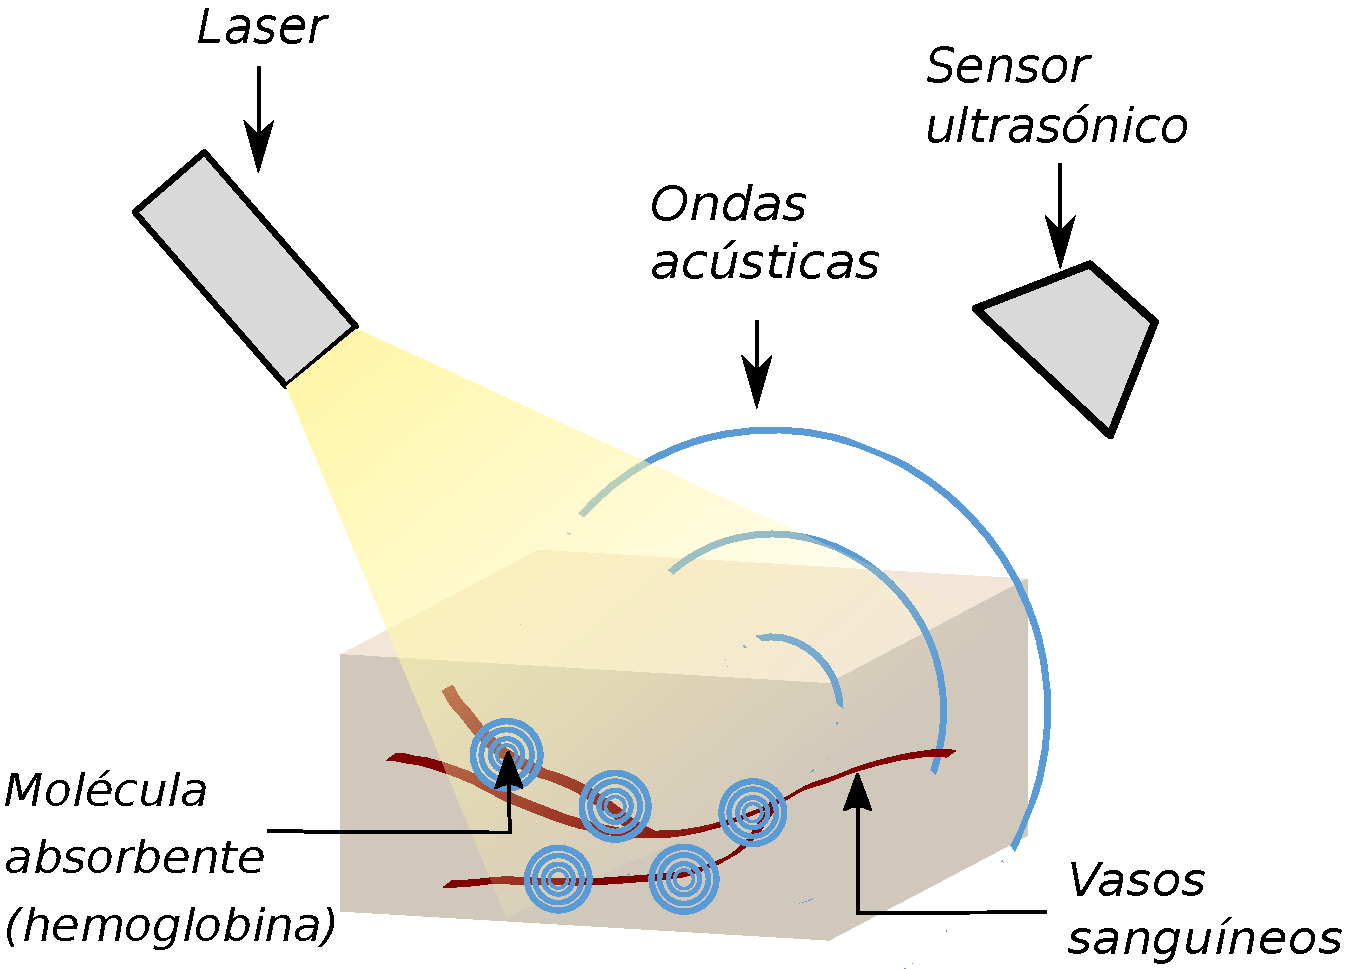
\includegraphics[width=\textwidth]{Images/effect.pdf}
    \caption{Efecto fotoacústico.}
    \label{fig:efecto_fotoacustico}
\end{figure}

Las aplicaciones clínicas actuales incluyen la detección temprana de cáncer, imagen funcional cerebral, y caracterización vascular, entre otras \cite{kim2021clinical}. Los avances recientes en tecnología de sensores y sistemas de adquisición han mejorado significativamente la calidad y velocidad de adquisición de datos fotoacústicos \cite{zhang2020advances}.
\subsection{Métodos Tradicionales de Reconstrucción} \label{sec:lit:first:two}
Los métodos convencionales de reconstrucción fotoacústica se pueden clasificar en tres categorías principales \cite{kuchment2008mathematics}:

Los métodos analíticos, como la retroproyección filtrada y las técnicas de transformada de Fourier, proporcionan soluciones directas basadas en la ecuación de onda fotoacústica \cite{xu2005universal}. Estos métodos son computacionalmente eficientes pero pueden generar artefactos significativos en condiciones no ideales.

Los métodos iterativos, incluyendo técnicas de optimización variacional y métodos algebraicos, ofrecen mayor flexibilidad para incorporar información a priori y restricciones físicas \cite{huang2013full}. Sin embargo, su alto costo computacional limita su aplicabilidad en escenarios clínicos en tiempo real.

Los métodos basados en modelos incorporan explícitamente la física del problema mediante simulaciones numéricas detalladas \cite{cox2009challenges}. Aunque precisos, estos métodos requieren un conocimiento exacto de los parámetros físicos del medio y son computacionalmente intensivos.

% -----------------------------------------------------
\section{Importancia de la Consistencia Física en Reconstrucción Fotoacústica}

La consistencia física en la reconstrucción de imágenes fotoacústicas ha emergido como un aspecto crítico para obtener resultados robustos y fiables \cite{hauptmann2018model}. Esta importancia se fundamenta en múltiples aspectos que impactan tanto la calidad de la reconstrucción como la fiabilidad del resultado para aplicaciones prácticas.


\subsection{Naturaleza del Problema Inverso}
El problema inverso fotoacústico es inherentemente mal condicionado \cite{wang2009inverse}, lo que significa que pequeñas perturbaciones en los datos de entrada (señales acústicas) pueden resultar en grandes variaciones en la solución. La incorporación de restricciones físicas actúa como una forma natural de regularización \cite{arridge2016solving}, ayudando a:

\begin{itemize}
    \item Reducir el espacio de soluciones posibles a aquellas que son físicamente plausibles.
    \item Estabilizar el proceso de reconstrucción frente al ruido y las incertidumbres en las mediciones \cite{antholzer2019deep}.
    \item Mejorar la unicidad de la solución al incorporar información a priori sobre el comportamiento físico del sistema.
\end{itemize}

\subsection{Garantías de Validez y Robustez}
La consistencia física proporciona garantías importantes sobre la validez de las reconstrucciones \cite{shan2019physics}:

\begin{itemize}
    \item Asegura que las imágenes reconstruidas no solo sean visualmente plausibles, sino que también representen estados físicamente posibles del sistema.
    \item Permite verificar que la reconstrucción obedece las leyes fundamentales de la fotoacústica, como la ecuación de onda y las condiciones de contorno \cite{tick2016image}.
    \item Mejora la robustez del método, especialmente en casos con datos limitados o ruidosos \cite{hauptmann2020deep}.
\end{itemize}

\subsection{Ventajas en el Aprendizaje Profundo}
En el contexto del aprendizaje profundo, la incorporación de la física ofrece ventajas significativas \cite{raissi2019physics}:

\begin{itemize}
    \item Reduce la dependencia de grandes conjuntos de datos de entrenamiento al incorporar conocimiento previo sobre la física del problema \cite{hoffer2019augmented}.
    \item Proporciona una guía natural para el proceso de optimización, ayudando a la red a converger a soluciones más significativas \cite{zhou2020physics}.
    \item Permite detectar y corregir reconstrucciones que, aunque visualmente plausibles, violan las leyes físicas fundamentales del sistema.
\end{itemize}


\section{Deep Learning en Reconstrucción de Imágenes Fotoacústicas}

El aprendizaje profundo ha demostrado un éxito extraordinario en reconstrucción de imágenes fotoacústicas, particularmente con la arquitectura U-Net. Sin embargo, un desafío fundamental persiste: cómo incorporar efectivamente el conocimiento físico del problema en el proceso de aprendizaje.

\subsection{Evolución de Métodos de Reconstrucción con Deep Learning}

Las primeras aproximaciones utilizaban redes neuronales como post-procesamiento para mejorar imágenes reconstruidas con métodos tradicionales. Sin embargo, trabajos recientes como el de Guan et al. \cite{guan2020fully}, han demostrado que las arquitecturas densamente conectadas pueden abordar directamente el problema de reconstrucción, especialmente en casos de muestreo disperso donde los métodos tradicionales generan artefactos significativos.

\subsection{Incorporación de Física en Redes Neuronales}

La incorporación de conocimiento físico en redes neuronales ha seguido principalmente dos enfoques:

\begin{itemize}
\item \textbf{Physics-Informed Neural Networks (PINNs):} Incorporan directamente las ecuaciones diferenciales en la función de pérdida. Sin embargo, como se discute en \cite{Zhou2024DataGuided}, estos métodos pueden enfrentar desafíos durante el entrenamiento debido al desbalance entre los términos de pérdida física y de datos.

\item \textbf{Data-Guided Physics-Informed Approaches:} Propuestos más recientemente, estos métodos buscan un balance entre el aprendizaje basado en datos y las restricciones físicas. El trabajo de Zhou et al. \cite{Zhou2024DataGuided} introduce un marco de trabajo en dos fases que primero optimiza la pérdida de datos y luego incorpora gradualmente las restricciones físicas.
\end{itemize}

\subsection{Desafíos en la Incorporación de Física}

La incorporación de restricciones físicas en redes neuronales para reconstrucción fotoacústica presenta varios desafíos únicos:

\begin{itemize}
\item \textbf{Complejidad Computacional:} Los métodos PINN tradicionales requieren la evaluación de derivadas durante el entrenamiento, lo que aumenta significativamente el costo computacional.

\item \textbf{Balance de Pérdidas:} Como se evidencia en \cite{Zhou2024DataGuided}, mantener un balance adecuado entre la pérdida de datos y las restricciones físicas es crucial para el entrenamiento efectivo.

\item \textbf{Naturaleza Mal Condicionada:} El problema inverso en fotoacústica es inherentemente mal condicionado, lo que complica la incorporación de restricciones físicas.
\end{itemize}

\section{Limitaciones y Desafíos Actuales}

Los métodos actuales de incorporación de física en redes neuronales enfrentan varios desafíos:

\begin{itemize}
\item \textbf{Eficiencia Computacional:} Los PINN tradicionales son computacionalmente costosos, limitando su aplicabilidad en escenarios clínicos.

\item \textbf{Generalización:} La mayoría de los conjuntos de datos son simulados, planteando preguntas sobre la generalización a casos reales.

\item \textbf{Validación:} La evaluación de la consistencia física en las reconstrucciones requiere métricas específicas que van más allá de las medidas de calidad de imagen tradicionales.
\end{itemize}

Estos desafíos motivan la búsqueda de nuevos enfoques que puedan mantener la consistencia física mientras son computacionalmente eficientes y robustos en aplicaciones reales.

%%%%% ------- Methodology ------- %%%%%
\maincontent{Metodología}
En esta sección se presenta la metodología de este trabajo tanto teórica como experimental. Partiendo desde la matemática del problema hasta la arquitectura de las redes neuronales utilizadas. En esta sección se presenta la metodología de este trabajo tanto teórica como experimental. Partiendo desde la matemática del problema hasta la arquitectura de las redes neuronales utilizadas. Se describen las variables de estudio, las métricas de evaluación y el proceso de entrenamiento.

\section{Fundamentos Teóricos} \label{sec:fundamentos}

Primero comenzamos por entender el problema físico subyacente y por qué es importante tener en cuenta la consistencia física en la reconstrucción de imágenes fotoacústicas y cómo es que esta consistencia física puede ayudar a nuestra red neuronal a aprender de manera más eficiente y a obtener mejores resultados.

La solución del problema inverso del efecto fotoacústico es una función de distribución a la cual llamamos imagen. Existen dos métodos muy populares para resolver el problema inverso: "Time Reversal" y "Back Projection", los cuales se derivan de suposiciones físicas y matemáticas, lo cual es conocido como DAS (Delay and Sum).

\subsection{Efecto Fotoacústico}

El efecto fotoacústico es la generación de una onda ultrasónica que es producida por un material fotosensible al ser iluminado por un pulso de luz. 

La generación y propagación de la onda fotoacústica es modelada por la ecuación para un fluido ideal y está muy bien descrita por el acoplamiento de la ecuación de difusión de calor para la variación de temperatura $T(\mathbf{x}, t)$ (\textit{ec}. \ref{diffusionequation}) y la ecuación de onda acústica para la presión $P(\mathbf{x}, t)$ (\textit{ec.} \ref{waveequation}).

\begin{equation}
    (\chi \nabla^2  - \frac{\partial}{\partial t})T(\mathbf{x}, t) = - \frac{1}{\rho_{0}C_{P}}H(\mathbf{x}, t)
    \label{diffusionequation}
\end{equation}

\begin{equation}
    (\frac{1}{K_{T}\rho_{0}}\nabla^2 - \frac{\partial^2}{\partial t^2})P(\mathbf{x}, t) = -\frac{\beta}{K_{T}}\frac{\partial^2}{\partial^2 t}T(\mathbf{x}, t)
    \label{waveequation}
\end{equation}

donde, para la muestra, $\chi$ es la conductividad térmica, $\rho_{0}$ es la densidad, $C_{P}$ es el calor específico, $H(\mathbf{x}, t)$ es la densidad de energía electromagnética por unidad de tiempo absorbida por la muestra, $K_{T}$ es el coeficiente de compresibilidad térmica, y $\beta$ es el coeficiente de expansión térmica.

La densidad de energía electromagnética $H(\mathbf{x}, t)$ es modelada como:

\begin{equation}
    H({\mathbf{x}^{\prime}}, t) = \mu({\mathbf{x}^{\prime}}, t)\phi({\mathbf{x}^{\prime}}, t)
\end{equation}

donde $\mathbf{x}^{\prime}$ es la posición de la fuente de la onda, $\mu(\mathbf{x}^{\prime}, t)$ es el coeficiente de absorción óptico de la muestra y $\phi(\mathbf{x}^{\prime}, t)$ es la tasa de fluencia del pulso láser. La tasa de fluencia puede ser descrita como el producto de la intensidad $I(\mathbf{x}^{\prime})$ y el perfil temporal $\theta(t)$ del pulso láser $\phi(\mathbf{x}^{\prime}, t) = I(\mathbf{x}^{\prime})\theta(t)$.

\subsection{Ecuación de Onda Fotoacústica}
La ecuación de onda fotoacústica modela la propagación de la onda acústica generada $P(\mathbf{x}, t)$ producida por la expansión termoelástica de la muestra.

Esta ecuación se obtiene desacoplando las ecuaciones \ref{diffusionequation} y \ref{waveequation}. Existen suposiciones físicas acerca del medio donde la onda se propaga, como la viscosidad, la absorción acústica es ignorada, la variación de la presión y densidad son pequeñas comparadas a los valores iniciales y la velocidad de las partículas es menor que la velocidad del sonido entre otras, que permiten simplificar la ecuación de onda acústica a:

\begin{equation}
    \left[\nabla^2 p - \frac{1}{c^2}\frac{\partial^2 }{\partial t^2}\right]P(\mathbf{x}, t) = -\frac{\beta}{C_p}\frac{\partial H}{\partial t}
\end{equation}

donde $c$ es la velocidad del sonido en el medio de propagación, y es definida como $c = \left(K_{T}\rho_{0}\frac{\beta^2 T_{0}}{C_{P}}\right)^{-1}$.

\subsection{Problema Inverso del Efecto Fotoacústico}
El problema inverso fotoacústico (PA) implica resolver un problema de valor en la frontera para la ecuación de onda PA. La solución proporciona la distribución espacial de la absorción electromagnética durante el proceso de expansión termoelástica.

Para definir el problema inverso PA, se asume que la densidad de energía electromagnética absorbida por la muestra, $H(\mathbf{x}',t)$, es separable en componentes espaciales y temporales:
\begin{equation}
    H(\mathbf{x}',t) = h_x(\mathbf{x}') h_t(t).
\end{equation}

Para un tiempo de iluminación $\tau_p$ corto (tal que $\tau_p \ll 1/\mu c$), la función temporal puede aproximarse mediante una función delta de Dirac:
\begin{equation}
    h_t \to \delta(t) \quad \text{cuando} \quad \Delta T \to 0.
\end{equation}

Esta condición, conocida como la \textit{condición de confinamiento de estrés}, asume que la transferencia de calor ocurre antes de que haya cambios significativos en la densidad de masa.

Cuando la muestra absorbe energía electromagnética, las variaciones de temperatura inducen cambios en la densidad de masa y la presión. Utilizando relaciones termodinámicas, la distribución de presión inicial se expresa como:
\begin{equation}
    P|_{t=0} = \frac{\beta}{K_T} T|_{t=0} = \Gamma h_x,
\end{equation}
donde $\Gamma$ es el parámetro de Grüneisen, que describe la eficiencia del proceso de conversión de calor a presión.

Para imponer el confinamiento de estrés y la distribución inicial de presión, se resuelve la ecuación de onda con un término fuente:
\begin{equation}
    \left[ \nabla^2 - \frac{1}{c^2} \frac{\partial^2}{\partial t^2} \right] P = 0, \quad \text{con} \quad P(\mathbf{x}, 0) = \Gamma h_x, \quad \frac{\partial P}{\partial t} \Big|_{t=0} = 0.
\end{equation}

El problema inverso PA se formula utilizando condiciones de frontera en una superficie de observación $S$ donde se miden los valores de presión:
\begin{equation}
    \left[ \nabla^2 - \frac{1}{c^2} \frac{\partial^2}{\partial t^2} \right] P(\mathbf{x},t) = 0, \quad t \geq 0,
\end{equation}
\begin{equation}
    P(\mathbf{x}', 0) = f(\mathbf{x}'), \quad \frac{\partial P}{\partial t} \Big|_{t=0} = 0,
\end{equation}
\begin{equation}
    P(\mathbf{x}_S, t) = g(\mathbf{x}_S, t), \quad \mathbf{x}_S \in S, \quad t \geq 0.
\end{equation}

El objetivo es determinar la distribución de presión inicial $f(\mathbf{x}')$ a partir de los datos de frontera $g(\mathbf{x}_S, t)$. Esta distribución representa la imagen PA.

Los supuestos matemáticos para garantizar la resolubilidad incluyen:
\begin{itemize}
    \item La fuente está contenida dentro de $S$.
    \item No existen fuentes PA externas.
    \item La ecuación de onda es válida en todo el espacio.
\end{itemize}

Debido a la naturaleza termodinámica del efecto fotoacústico, el problema inverso PA es mal condicionado, lo que ha llevado al desarrollo de métodos de regularización, entre otros.

\subsection{Deep Learning en Reconstrucción Fotoacústica}

El uso de redes neuronales profundas en la reconstrucción de imágenes fotoacústicas se ha implementado de diferentes formas, tanto complementando una reconstrucción inicial con métodos clásicos como el DAS y removiendo los artefactos que este genera \cite{guan2020fully}, como también desde cero, tomando datos en crudo y generando imágenes a partir de estos \cite{Yang2021}.

Muchos de estos trabajos usan la popular arquitectura U-Net \cite{ronneberger2015unet} para la reconstrucción de imágenes, la cual ha demostrado ser muy efectiva en la reconstrucción de imágenes en diferentes campos de la ciencia. Sin embargo, la mayoría de estos trabajos no toman en cuenta la consistencia física de las imágenes reconstruidas, sin contar aquellos que complementan deep learning con métodos clásicos.

La consistencia física, si bien no parece ser un problema al momento de reconstruir la imagen a partir de la onda acústica, puede ser usada para enseñar a la red a realizar la reconstrucción de manera más eficiente y con mejores resultados, ya que la red puede aprender de manera implícita las características físicas del problema.

Como ya mencioné, el problema inverso del efecto fotoacústico es mal condicionado. Se han desarrollado métodos de aprendizaje profundo para resolver este tipo de problemas como los Physics Informed Neural Networks (PINNs) \cite{Raissi2017Physics} que son redes neuronales que son entrenadas para resolver ecuaciones diferenciales parciales. Sin embargo, estos métodos no han sido aplicados en la reconstrucción de imágenes fotoacústicas directamente; si bien lo que hacen es poder encontrar los parámetros de una ecuación diferencial parcial, no se ha aplicado directamente a la reconstrucción de imágenes. Sin embargo, enfoques interesantes han surgido a partir de esta idea, como hacer un fine-tuning de una red ya preentrenada primero minimizando puramente la pérdida relacionada a los datos, después minimizando las pérdidas relacionadas tanto a los datos como a la pérdida residual de la PDE \cite{Zhou2024DataGuided}. Sin embargo, como mencioné, estos trabajos no se concentran principalmente en la reconstrucción de las imágenes fotoacústicas, pero sí dan un sentido de cómo se puede incorporar la física en las redes neuronales haciendo el preentrenamiento de la red con datos y después con la física, mejorando las soluciones para problemas inversos mal condicionados.

\section{Enfoque Propuesto}
\label{sec:enfoque}

El método propuesto se basa en un enfoque dual que combina dos redes neuronales U-Net con roles complementarios: una red reconstructora y una red supervisora. Este diseño está motivado por la necesidad de incorporar consistencia física en el proceso de reconstrucción de imágenes fotoacústicas. La arquitectura general se muestra en la Figura \ref{fig:fine-tuning}.


\begin{figure}
    \centering
    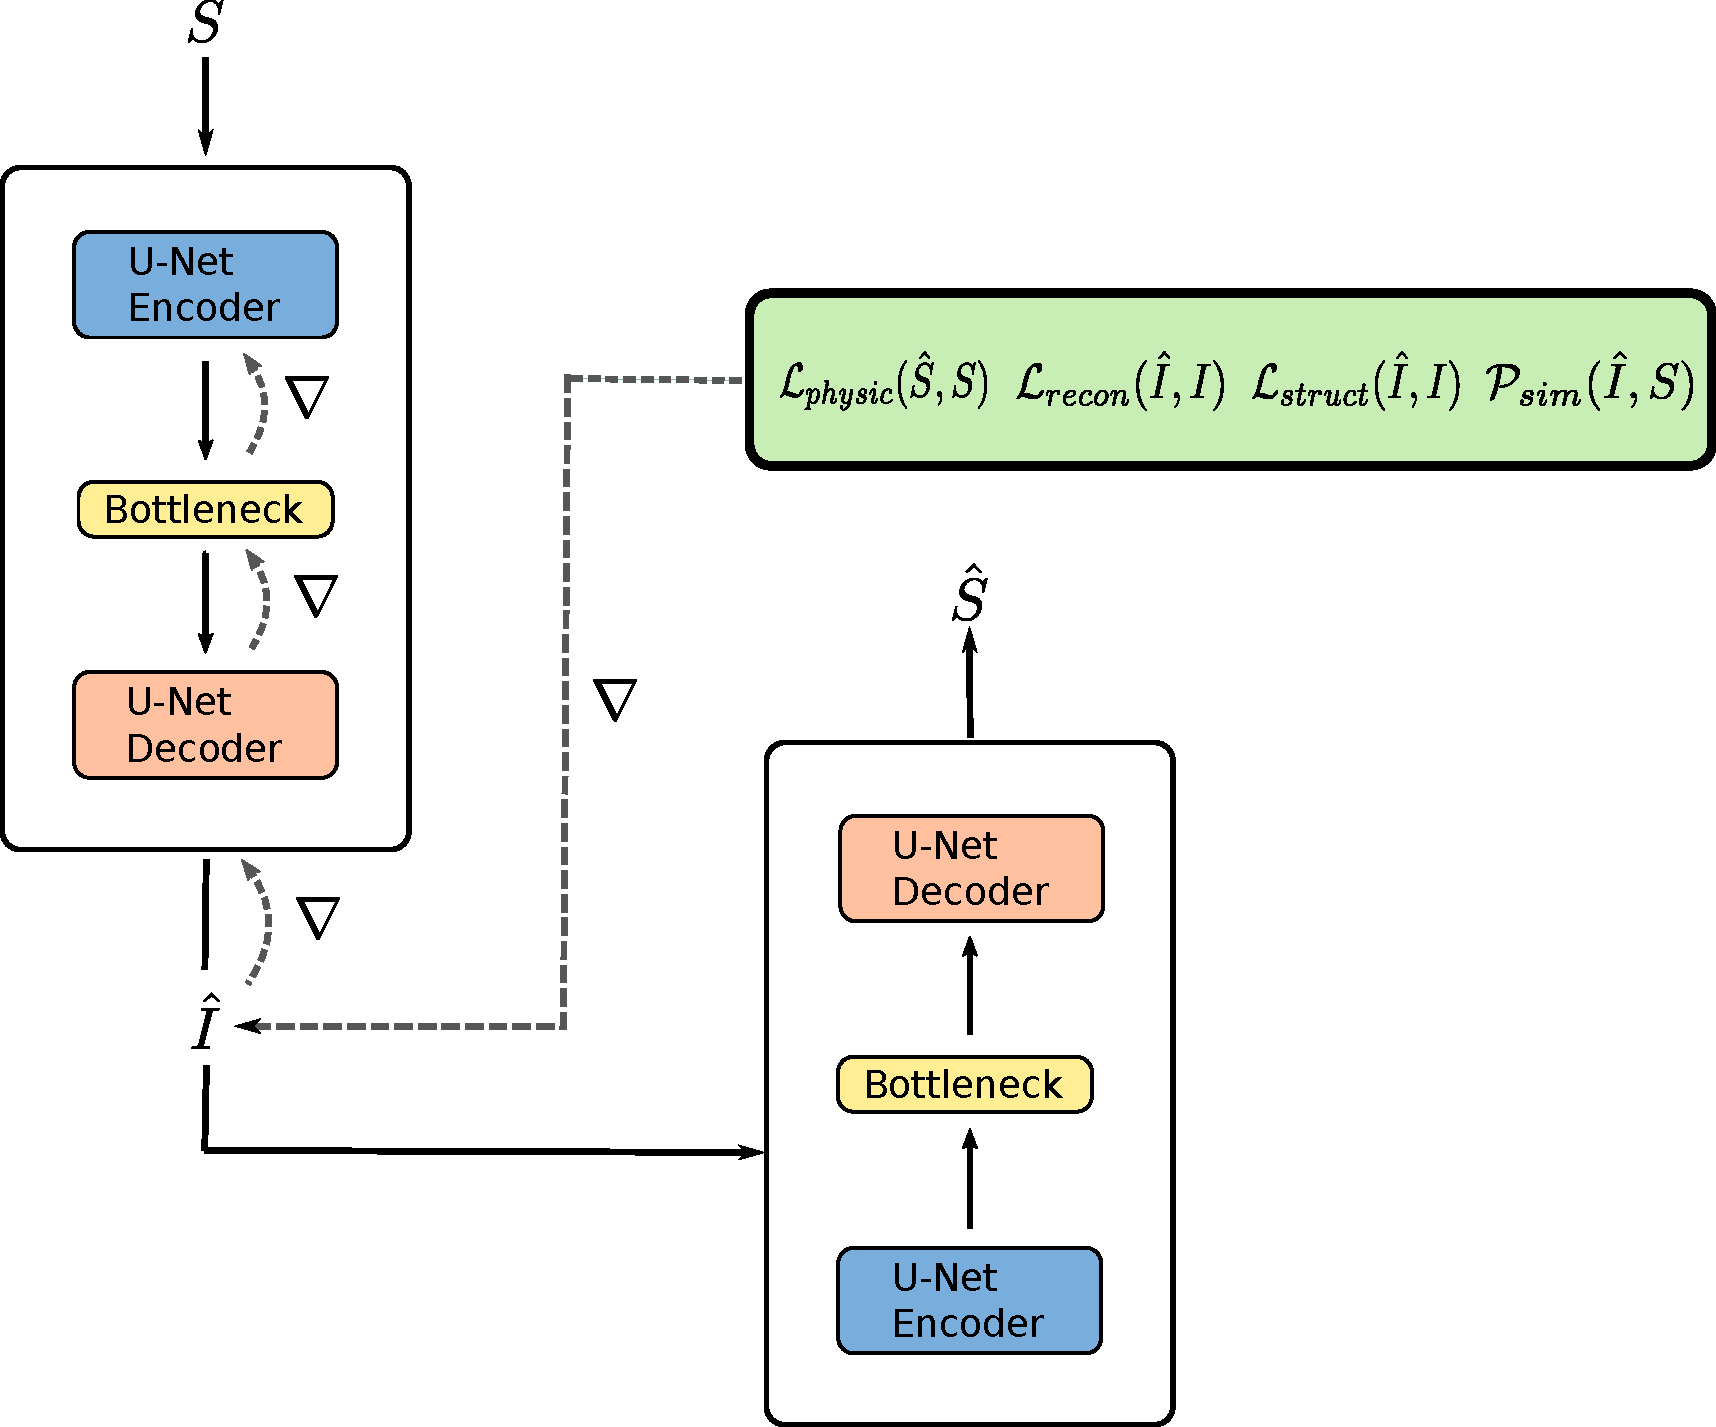
\includegraphics[width=0.8\textwidth]{Images/arq.pdf}
    \caption{Arquitectura de la red propuesta. La red reconstructora se entrena para aprender el mapeo directo de señales acústicas a imágenes fotoacústicas. La red supervisora se entrena para emular el proceso físico de generación de señales acústicas a partir de una imagen dada. Durante el proceso de fine-tuning, la red reconstructora se entrena para generar imágenes que, al ser procesadas por la red supervisora, produzcan señales acústicas consistentes con las mediciones originales.}
    \label{fig:fine-tuning}
\end{figure}

La red reconstructora tiene como objetivo principal transformar las señales acústicas medidas ($S$) en imágenes fotoacústicas ($\hat{I}$), mientras que la red supervisora actúa como un evaluador físico, aprendiendo a simular el proceso de generación de señales acústicas a partir de una imagen dada. La clave de este enfoque es el entrenamiento en dos fases: un preentrenamiento individual de cada red seguido de un proceso de fine-tuning que incorpora la supervisión física.

\subsection{Arquitectura del Sistema}

Ambas redes siguen una arquitectura U-Net modificada que consiste en:
\begin{itemize}
    \item Un codificador (Encoder) que extrae características relevantes de la entrada
    \item Un cuello de botella (Bottleneck) que comprime la información
    \item Un decodificador (Decoder) que reconstruye la salida deseada
\end{itemize}

\subsection{Preentrenamiento Individual}

El preentrenamiento se realiza de manera independiente para cada red, estableciendo las capacidades básicas necesarias para el proceso de fine-tuning posterior.

\subsubsection{Red Reconstructora}
La red reconstructora se entrena para aprender el mapeo directo de señales acústicas a imágenes fotoacústicas. Durante esta fase, la red optimiza:

\begin{equation}
    \mathcal{L}_A = \text{MSE}(\hat{I}, I)
\end{equation}

donde $\hat{I}$ es la imagen reconstruida y $I$ es la imagen objetivo. Esta pérdida asegura que la red aprenda a generar reconstrucciones visualmente precisas.

\subsubsection{Red Supervisora}
La red supervisora se entrena para aproximar el proceso físico de generación de señales acústicas. Este proceso puede ser modelado como:

\begin{equation}
    S = \mathcal{F}(I) + \epsilon
\end{equation}

donde $\mathcal{F}$ representa una aproximación del operador físico de propagación fotoacústica. En la práctica, este operador encapsula las complejas relaciones descritas por las ecuaciones de onda fotoacústica presentadas en la sección \ref{sec:fundamentos}. La red neuronal actúa como un aproximador universal de esta función, aprendiendo a mapear las imágenes a sus correspondientes señales acústicas sin necesidad de resolver explícitamente las ecuaciones diferenciales parciales subyacentes. El término $\epsilon$ modela tanto el ruido del sistema como los errores de aproximación inherentes a este enfoque.

La red optimiza:
\begin{equation}
    \mathcal{L}_B = \text{MSE}(\hat{S}, S)
\end{equation}

donde $S_{pred}$ es la señal acústica predicha por la red y $S_{true}$ es la señal acústica medida. Este entrenamiento permite a la red supervisora aprender implícitamente las características físicas del proceso fotoacústico, actuando como un simulador aprendido del sistema físico.

\subsection{Flujo de Datos}

Durante el proceso de reconstrucción, los datos fluyen de la siguiente manera:
\begin{enumerate}
    \item La señal acústica $S$ ingresa a la red reconstructora
    \item La red reconstructora genera una imagen reconstruida $\hat{I}$
    \item Esta imagen es procesada por la red supervisora para generar una señal acústica predicha $\hat{S}$
    \item Las diferentes pérdidas se calculan comparando las salidas con los valores objetivo
\end{enumerate}

Este diseño permite que la red reconstructora aprenda no solo de la comparación directa con las imágenes objetivo, sino también de la retroalimentación proporcionada por la red supervisora a través de la consistencia física de las señales acústicas generadas.

\subsection{Fine-tuning con Supervisión Física}

El proceso de fine-tuning se realiza sobre la red reconstructora previamente entrenada, incorporando un mecanismo de supervisión física a través de la red supervisora. Este proceso está diseñado para asegurar que las imágenes reconstruidas no solo sean visualmente precisas, sino que también mantengan consistencia con las propiedades físicas del sistema fotoacústico.

La estructura del fine-tuning involucra cuatro términos de pérdida complementarios:

\begin{equation}
    \mathcal{L}_{total} = \lambda_{1} \mathcal{L}_{recon} + \lambda_{2} \mathcal{L}_{physics} + \lambda_{3} \mathcal{L}_{struct} + \lambda_{4} \mathcal{P}_{sim}
\end{equation}

donde:

\begin{itemize}
    \item $\mathcal{L}_{recon}$ mide la discrepancia entre la imagen reconstruida $\hat{I}$ y la imagen objetivo $I$:
    \begin{equation}
        \mathcal{L}_{recon} = \text{MSE}(\hat{I}, I)
    \end{equation}
    
    \item $\mathcal{L}_{physics}$ evalúa la consistencia física comparando la señal acústica predicha $\hat{S}$ con la señal real $S$:
    \begin{equation}
        \mathcal{L}_{physics} = \text{MSE}(\hat{S}, S)
    \end{equation}
    
    \item $\mathcal{L}_{struct}$ preserva las características estructurales de la imagen:
    \begin{equation}
        \mathcal{L}_{struct} = 1 - \text{SSIM}(\hat{I}, I)
    \end{equation}
    
    \item $\mathcal{P}_{sim}$ es un término de penalización que previene que la red tome atajos durante el aprendizaje:
    \begin{equation}
        \mathcal{P}_{sim} = \text{cos\_similarity}(\hat{I}, S)
    \end{equation}
\end{itemize}

Los coeficientes $\lambda_i$ ponderan la contribución de cada término en la pérdida total. Durante el fine-tuning, la red supervisora se mantiene con sus pesos congelados, actuando como un evaluador fijo de la consistencia física de las reconstrucciones. Esta red toma la imagen reconstruida $\hat{I}$ y genera una predicción de la señal acústica $\hat{S}$ que debería producir dicha imagen.

El término $\mathcal{L}_{physics}$ es particularmente importante ya que fuerza a la red reconstructora a generar imágenes que, cuando son procesadas por la red supervisora, producen señales acústicas consistentes con las mediciones originales. Esto asegura que la reconstrucción no solo sea visualmente precisa ($\mathcal{L}_{recon}$ y $\mathcal{L}_{struct}$) sino que también respete las propiedades físicas del sistema fotoacústico.

El término de penalización $\mathcal{P}_{sim}$ es crucial para evitar que la red tome atajos en el proceso de aprendizaje. Sin esta penalización, la red podría tender a generar imágenes que son similares a las señales de entrada, lo cual produciría señales acústicas similares a las originales (minimizando $\mathcal{L}_{physics}$) pero no representaría una reconstrucción válida del objeto original.

Este enfoque de fine-tuning permite que la red reconstructora refine sus predicciones incorporando conocimiento físico del sistema, mientras mantiene la calidad visual y estructural de las reconstrucciones. La combinación de los diferentes términos de pérdida asegura un balance entre la fidelidad de la reconstrucción y la consistencia física del resultado.


%%%%% ----- Implementation and Experiments ----- %%%%% % Separado en dos capítulos
\maincontent{Implementación}
Esta sección describe los detalles de la implementación del modelo del modelo U-Net para la recosntruccion de imagenes fotoacústicas. Se incluyen las especificaciones técnicas, hiperparámetros de entrenamiento, pipeline de entrenamiento y validación y pruebas realizadas.


\section{Especificaciones Técnicas}
Para la implementación del modelo U-Net se utilizó el framework de programación PyTorch. La implementación se realizó en Python 3.8.5 y se utilizó la versión 1.7.1 de PyTorch. El código fuente se encuentra disponible en el repositorio de GitHub.
\subsection{Arquitectura del Sistema}
\begin{table}[H]
    \centering
    \begin{tabular}{llll}
    \hline
    \textbf{Sección} & \textbf{Capa} & \textbf{Operación} & \textbf{Canales (in/out)} \\
    \hline
    \multirow{4}{*}{Encoder} 
    & enc1 & Double Conv + ReLU & 1 $\rightarrow$ 64 \\
    & enc2 & MaxPool + Double Conv + ReLU & 64 $\rightarrow$ 128 \\
    & enc3 & MaxPool + Double Conv + ReLU & 128 $\rightarrow$ 256 \\
    & enc4 & MaxPool + Double Conv + ReLU & 256 $\rightarrow$ 512 \\
    \hline
    Bottleneck & bottleneck & MaxPool + Double Conv + ReLU & 512 $\rightarrow$ 1024 \\
    \hline
    \multirow{4}{*}{Decoder}
    & dec4 & ConvTranspose + Concat + Double Conv & (1024+512) $\rightarrow$ 512 \\
    & dec3 & ConvTranspose + Concat + Double Conv & (512+256) $\rightarrow$ 256 \\
    & dec2 & ConvTranspose + Concat + Double Conv & (256+128) $\rightarrow$ 128 \\
    & dec1 & ConvTranspose + Concat + Double Conv & (128+64) $\rightarrow$ 64 \\
    \hline
    Salida & final & Conv 1x1 & 64 $\rightarrow$ 1 \\
    \hline
    \end{tabular}
    \caption{Arquitectura del modelo U-Net. Cada 'Double Conv' consiste en dos capas convolucionales 3x3 seguidas de BatchNorm y ReLU. Las operaciones ConvTranspose tienen kernel 2x2 y stride 2.}
    \label{tab:unet_architecture}
\end{table}

\subsection{Hiperparámetros de Entrenamiento}
Ya que el proceso esta divido en dos partes, preentrenamiento y fine-tuning, a continuación se presentan los hiperparámetros utilizados en el entrenamiento del modelo U-Net.

\subsubsection{Preentrenamiento} \label{subsubsec:pretraining}

El preentrenamiento tanto de la red constructora como la red supervisora se realizó con los siguientes hiperparámetros:

\begin{table}[H]
    \centering
    \begin{tabular}{ll}
    \hline
    \textbf{Hiperparámetro} & \textbf{Valor} \\
    \hline
    Optimizador & Adam \\
    Learning rate inicial & 0.001 \\
    Batch size & Determinado por dataloader \\
    Número de épocas & 150 (default) \\
    Scheduler & ReduceLROnPlateau \\
    Scheduler patience & 5 épocas \\
    Scheduler factor & 0.5 \\
    Función de pérdida & MSE \\
    \hline
    \end{tabular}
    \caption{Hiperparámetros utilizados en el entrenamiento del modelo}
    \label{tab:hyperparameters}
\end{table}

\subsubsection{Fine-tuning}

Para el fine-tuning de la red constructora se utilizó el siguiente conjunto de hiperparámetros:

\begin{table}[H]
    \centering
    \begin{tabular}{ll}
    \hline
    \textbf{Hiperparámetro} & \textbf{Valor} \\
    \hline
    Optimizador & Adam \\
    Learning rate inicial & 0.001 \\
    Número de épocas & 100 (default) \\
    Scheduler & ReduceLROnPlateau \\
    Scheduler patience & 5 épocas \\
    Scheduler factor & 0.5 \\
    Función de pérdida & MSE + Pérdida estructural + Pérdida física + Penalización similitud \\
    \hline
    \multicolumn{2}{l}{\textbf{Pesos de las pérdidas}} \\
    $\lambda_{direct}$ & 1.0 \\
    $\lambda_{physical}$ & 0.1 \\
    $\lambda_{struct}$ & 2.0 \\
    $\lambda_{similarity}$ & 0.3 \\
    \hline
    \textbf{Otros} & \\
    Gradiente clipping & 1.0 \\
    Seed & 42 \\
    \hline
    \end{tabular}
    \caption{Hiperparámetros del entrenamiento supervisado}
    \label{tab:hyperparameters_supervised}
\end{table}


\section{Pipeline de Entrenamiento}
El pipeline de entrenamiento se dividió en dos fases: preentrenamiento y fine-tuning. Cada fase se realizó de manera independiente para las redes constructora y supervisora. A continuación se describen los detalles de cada fase.
\subsection{Obtención de Datos}
La obtención de datos experimentales fotoacústicos es un proceso complejo y costoso. Por ello, se implementó un pipeline de datos simulados para el preentrenamiento y fine-tuning del modelo. Este proceso involucra la generación de imágenes sintéticas y el cálculo de sus correspondientes señales fotoacústicas mediante un modelo físico (detallado en el Apéndice). Este enfoque permitió generar un conjunto de datos robusto para el entrenamiento y validación del modelo.
\subsection{Preentrenamiento}
El proceso de preentrenamiento se realizó de manera independiente para las redes constructora y supervisora:
\begin{itemize}
\item \textbf{Red Constructora:} Se utilizó un conjunto de 5000 pares de imágenes simuladas de 128×128 píxeles.
\item \textbf{Red Supervisora:} Se emplearon 5000 pares de imágenes (128×128 píxeles) y sus correspondientes señales fotoacústicas.
\end{itemize}
En ambos casos, se implementó una división del dataset: 80\% para entrenamiento y 20\% para validación.
\subsection{Fine-tuning}
La fase de fine-tuning mantuvo la misma estructura de datos que el preentrenamiento, utilizando 5000 imágenes simuladas para cada red. La distribución del conjunto de datos se mantuvo en 80\% para entrenamiento y 20\% para validación, permitiendo una optimización específica de los pesos previamente entrenados.

\section{Métricas de Evaluación} \label{sec:metrics}

Para evaluar exhaustivamente el desempeño del modelo, utilizaremos métricas que cubren diferentes aspectos de la calidad de reconstrucción, eficiencia y significancia estadística:

\subsection{Calidad de Reconstrucción}
La calidad de las imágenes reconstruidas se evaluará mediante las siguientes métricas:

\begin{itemize}
    \item \textbf{Peak Signal-to-Noise Ratio (PSNR):} Mide la relación entre la máxima potencia posible de una señal y el ruido que afecta a su representación. Un PSNR más alto indica una mejor calidad de reconstrucción.
    
    \item \textbf{Normalized Root Mean Square Error (NRMSE):} Cuantifica la diferencia entre los valores predichos y observados, normalizada para facilitar comparaciones entre diferentes escalas de datos.
    
    \item \textbf{Structural Similarity Index (SSIM):} Evalúa la similitud estructural entre las imágenes reconstruidas y las originales, considerando luminancia, contraste y estructura.
    
    \item \textbf{Mean Absolute Error (MAE):} Proporciona una medida directa de la diferencia absoluta entre los valores predichos y reales.
\end{itemize}

\subsection{Rendimiento Computacional}
El rendimiento computacional se evaluará considerando:

\begin{itemize}
    \item \textbf{Tiempo de Reconstrucción:} Medido en milisegundos por imagen, evaluando la eficiencia computacional del modelo en inferencia.
    
    \item \textbf{Uso de Memoria:} Cuantifica los recursos computacionales requeridos durante la reconstrucción.
    
    \item \textbf{FLOPs:} Mide el número de operaciones de punto flotante, proporcionando una métrica independiente del hardware para la complejidad computacional.
\end{itemize}

\subsection{Análisis Estadístico}
Para validar la significancia y robustez de los resultados, implementaremos:

\begin{itemize}
    \item \textbf{Pruebas de Significancia:} Se utilizará la prueba t-pareada para comparar el rendimiento entre el preentrenamiento y fine-tuning, estableciendo un nivel de significancia $\alpha = 0.05$.
    
    \item \textbf{Intervalos de Confianza:} Se calcularán intervalos de confianza del 95% para todas las métricas de rendimiento, proporcionando una medida de la incertidumbre en nuestras estimaciones.
    
    \item \textbf{Pruebas de Normalidad:} Se aplicará el test Shapiro-Wilk para verificar la normalidad en la distribución de los errores de reconstrucción, validando los supuestos estadísticos de nuestros análisis.
\end{itemize}

Este conjunto integral de métricas nos permitirá evaluar no solo la calidad de las reconstrucciones y la eficiencia computacional, sino también la significancia estadística de las mejoras observadas, proporcionando una base sólida para la comparación con otros métodos de reconstrucción.

\maincontent{Experimentos y Resultados} % Nuevo capítulo
En esta sección se describen los experimentos realizados para evaluar la metodología propuesta. Se comparan los resultados obtenidos con la metodología propuesta con los obtenidos al entrenar solo la U-Net. Además, se evalúa la importancia de cada componente de la función de pérdida propuesta al eliminarlo del finetuning.


\section{Experimentos}
Ademas del entrenamiento de las dos redes U-Net (constructora y supervisora) con los hiperparámetros especificados en la seccion \ref{subsubsec:pretraining}, para comparar la metodología propuesta con el estado del arte (solo entrenando la U-Net) y para evaluar la importancia de cada componente en la funcion de perdida, se realizaron experimentos con diferentes configuraciones. En la Tabla \ref{tab:experiments} se muestran las diferentes configuraciones utilizadas en los experimentos.

\begin{table}[H]
    \centering
    \begin{tabular}{lccccc}
    \hline
    \textbf{Experimento} & $\lambda_{direct}$ & $\lambda_{physical}$ & $\lambda_{struct}$ & $\lambda_{similarity}$ & \textbf{Descripción} \\
    \hline
    Baseline & 1.0 & 0.1 & 2.0 & 0.3 & Configuración completa propuesta \\
    Sin pérdida estructural & 1.0 & 0.1 & 0.0 & 0.3 & Elimina pérdida de similitud estructural \\
    Sin pérdida física & 1.0 & 0.0 & 2.0 & 0.3 & Elimina restricción del modelo físico \\
    \hline
    \end{tabular}
    \caption{Configuraciones de los experimentos de ablación. Cada experimento evalúa la importancia de un componente específico de la función de pérdida al eliminarlo del entrenamiento mientras mantiene los demás términos constantes.}
    \label{tab:experiments}
\end{table}

\section{Resultados}

Presentamos los resultados del preentrenamiento de cada red y los resultados del fine-tuning de la red constructora. Se comparan los resultados obtenidos con la metodología propuesta con los obtenidos al entrenar solo la U-Net. Además, se evalúa la importancia de cada componente de la función de pérdida propuesta al eliminarlo del finetuning.

\subsection{Preentrenamiento}
 
Para el preentrenamiento de cada red tuvimos los siguientes resultados:

\subsubsection{Red Reconstructora}

El primer paso fue entrenar red reconstructora con los hiperparámetros especificados en la sección \ref{subsubsec:pretraining}. La Figura \ref{fig:reconstructor_pretraining} muestra la evolución de la función de pérdida durante el entrenamiento. Se observa que la función de pérdida comienza en aproximadamente 0.015 MSE y disminuye rápidamente durante las primeras épocas, estabilizándose alrededor de la época 80 en valores cercanos a 0.0005 MSE. La proximidad entre las curvas de entrenamiento y validación indica una generalización efectiva sin señales aparentes de sobreajuste, sugiriendo un aprendizaje estable y robusto del modelo.

\begin{figure}[H]
    \centering
    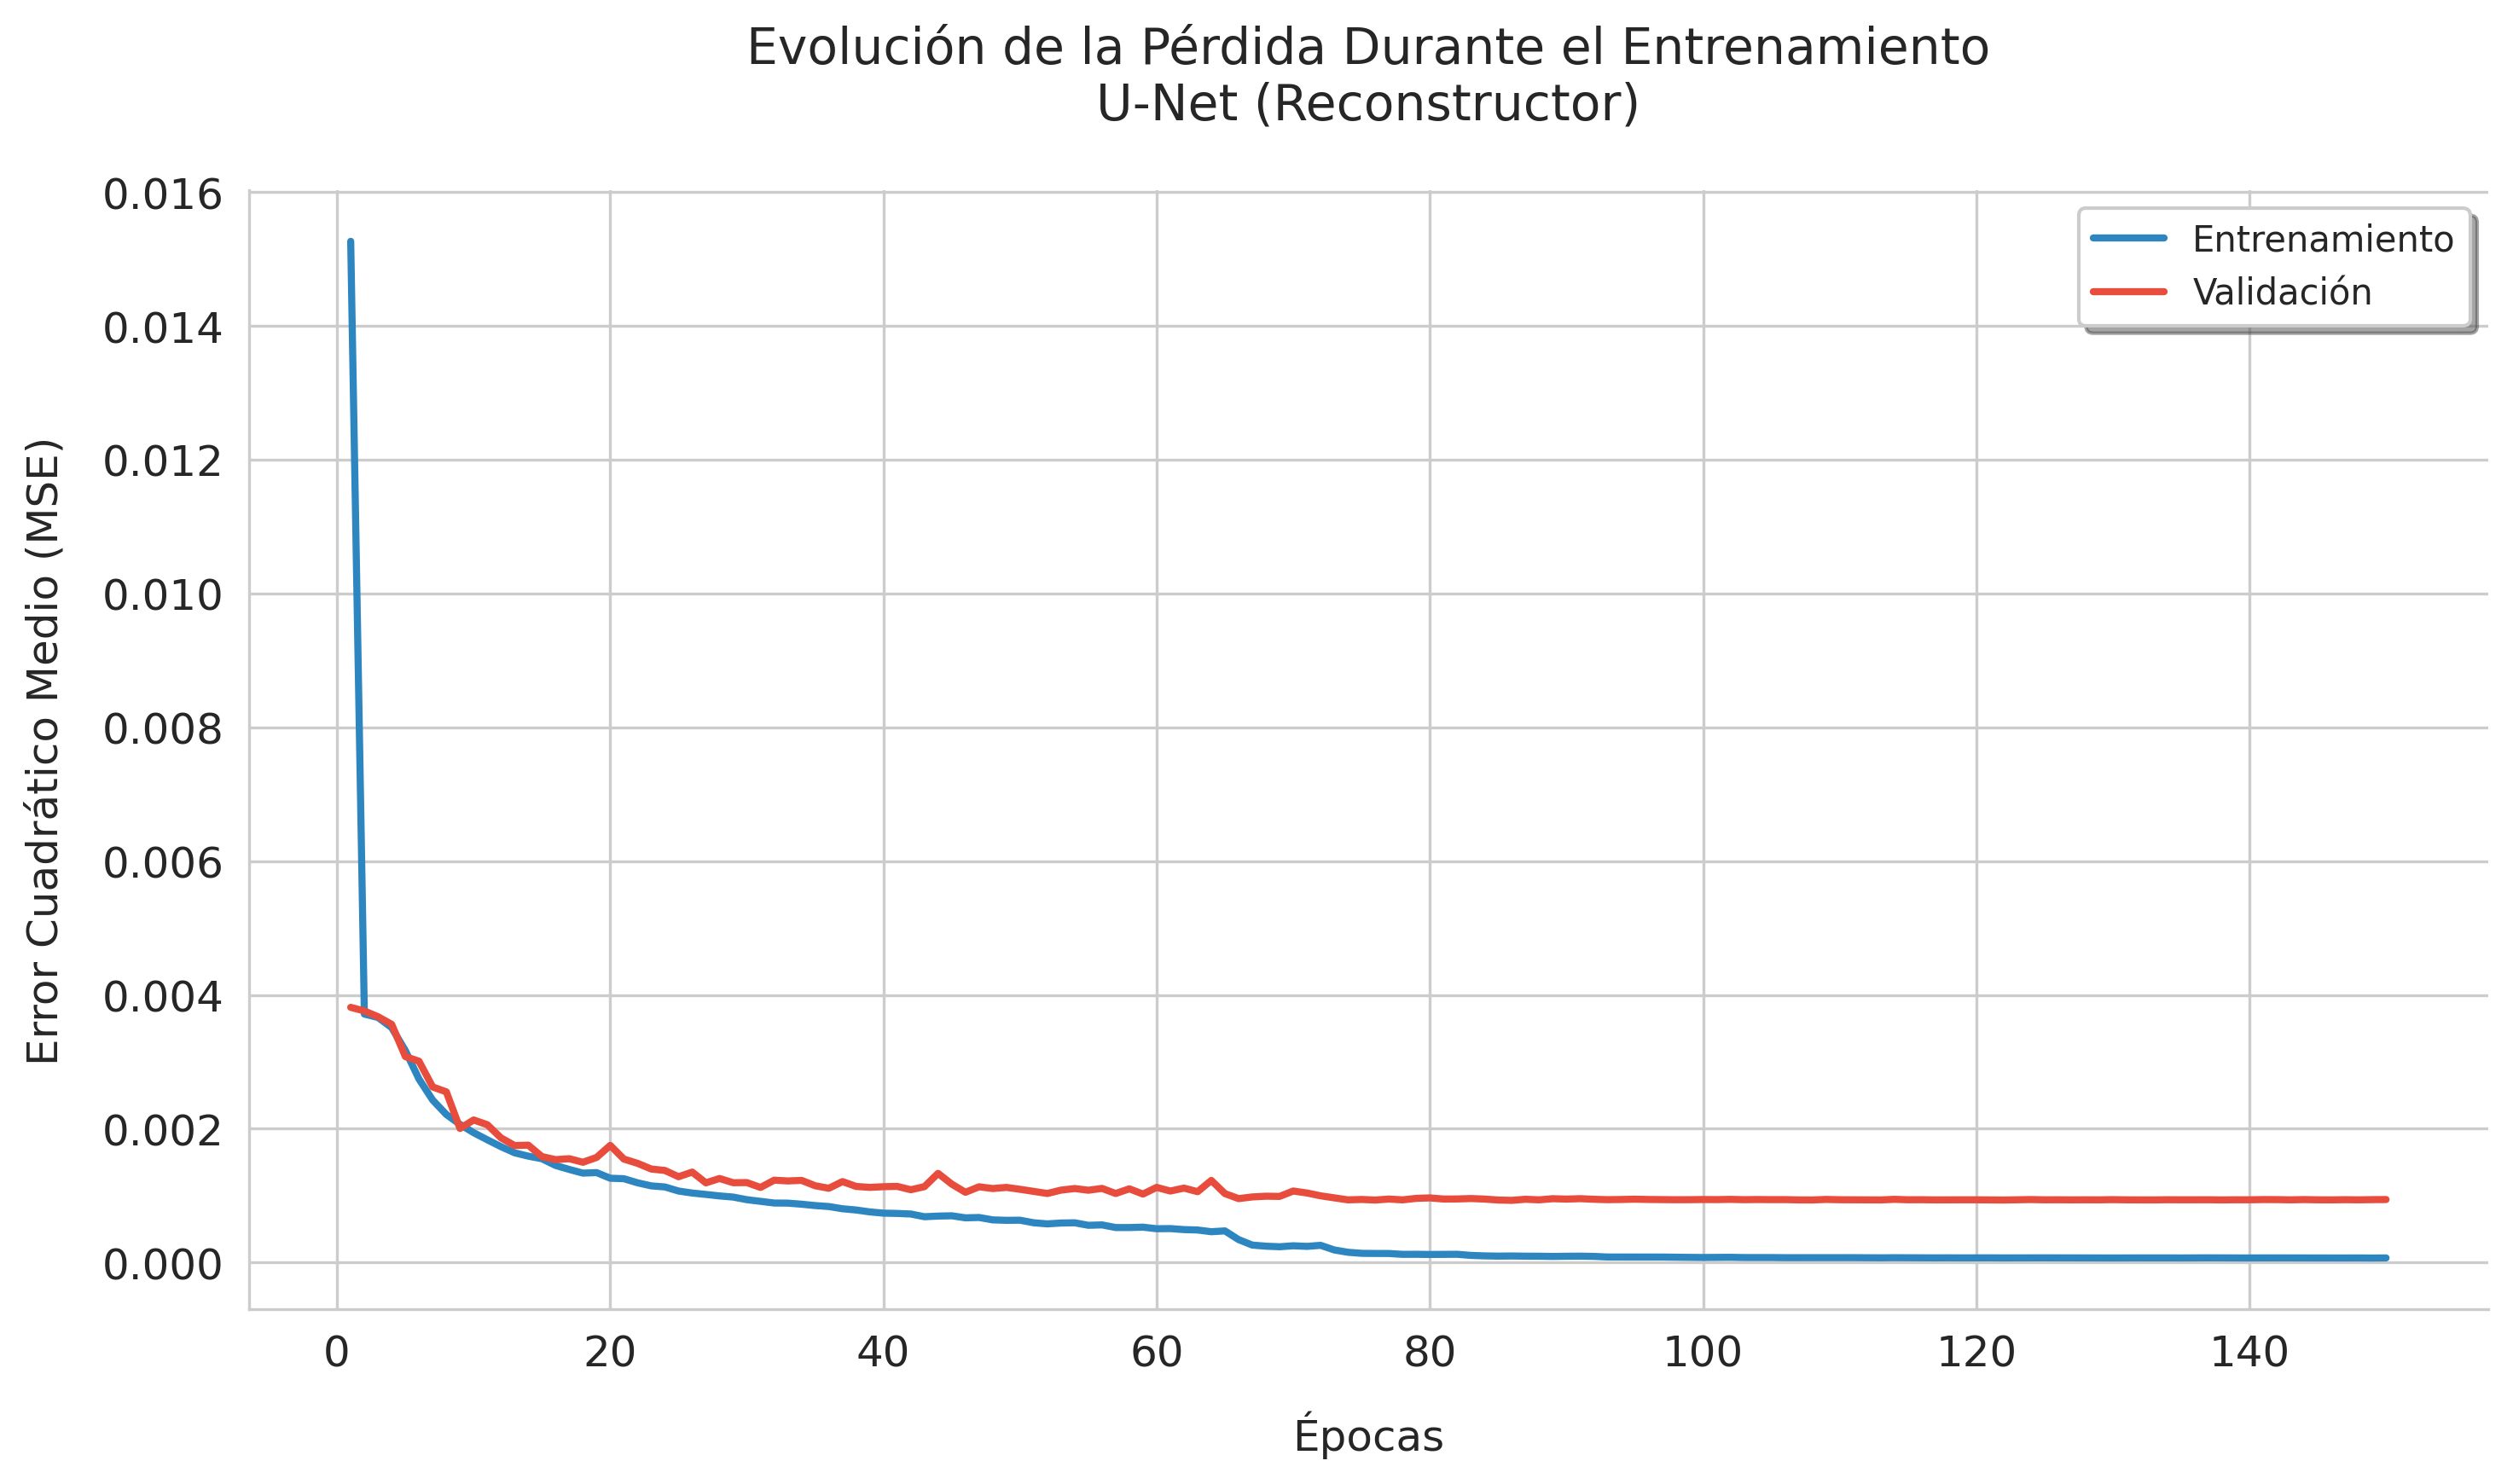
\includegraphics[width=0.8\textwidth]{Images/perdidas_entrenamiento_recon.png}
    \caption{Evolución de la función de pérdida durante el preentrenamiento de la red reconstructora.}
    \label{fig:reconstructor_pretraining}
\end{figure}

\subsubsection{Red Supervisora}

El segundo paso fue entrenar la red supervisora con los hiperparámetros especificados en la sección \ref{subsubsec:pretraining}. La Figura \ref{fig:supervisor_pretraining} muestra la evolución de la función de pérdida durante el entrenamiento. Se observa que la función de pérdida inicia en valores cercanos a 1.0 MSE y disminuye rápidamente durante las primeras épocas. Sin embargo, la curva de validación presenta fluctuaciones considerables durante el proceso de entrenamiento, convergiendo finalmente a un nivel de error más elevado (aproximadamente 0.1 MSE). La brecha más pronunciada entre las pérdidas de entrenamiento y validación, junto con las oscilaciones persistentes, sugieren que la tarea de supervisión presenta mayores desafíos en términos de generalización que la tarea de reconstrucción.

\begin{figure}[H]
    \centering
    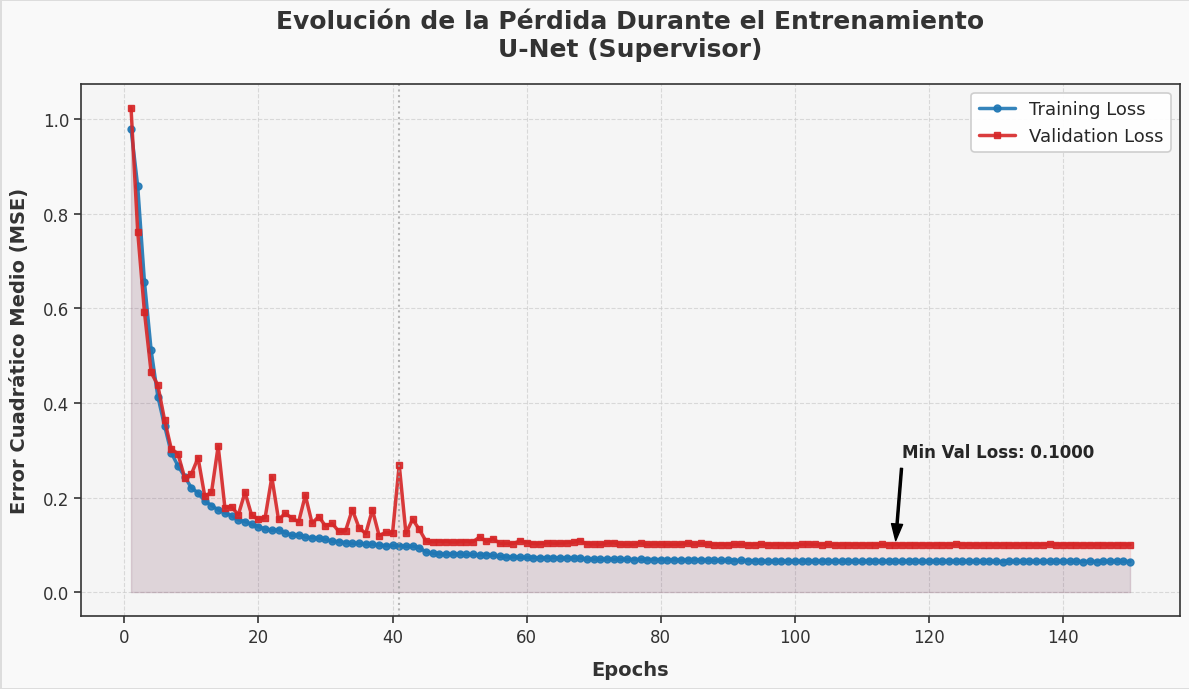
\includegraphics[width=0.8\textwidth]{Images/perdidas_entrenamiento_super.png}
    \caption{Evolución de la función de pérdida durante el preentrenamiento de la red supervisora.}
    \label{fig:supervisor_pretraining}
\end{figure}

\subsection{Fine-tuning}

Para evaluar la metodología propuesta, se realizó el fine-tuning de la red constructora con los hiperparámetros especificados en la sección \ref{subsubsec:pretraining}. Se comparan los resultados obtenidos con la metodología propuesta con los obtenidos al entrenar solo la U-Net. Además, se evalúa la importancia de cada componente de la función de pérdida propuesta al eliminarlo del finetuning.

\subsubsection{Metodología propuesta vs. U-Net}

Primero observamos los resultados obtenidos en el proceso del fine-tuning de la red reconstructora. La Figura \ref{fig:reconstructor_finetuning} muestra la evolución de la función de pérdida durante el entrenamiento. 

\begin{figure}[H]
    \centering
    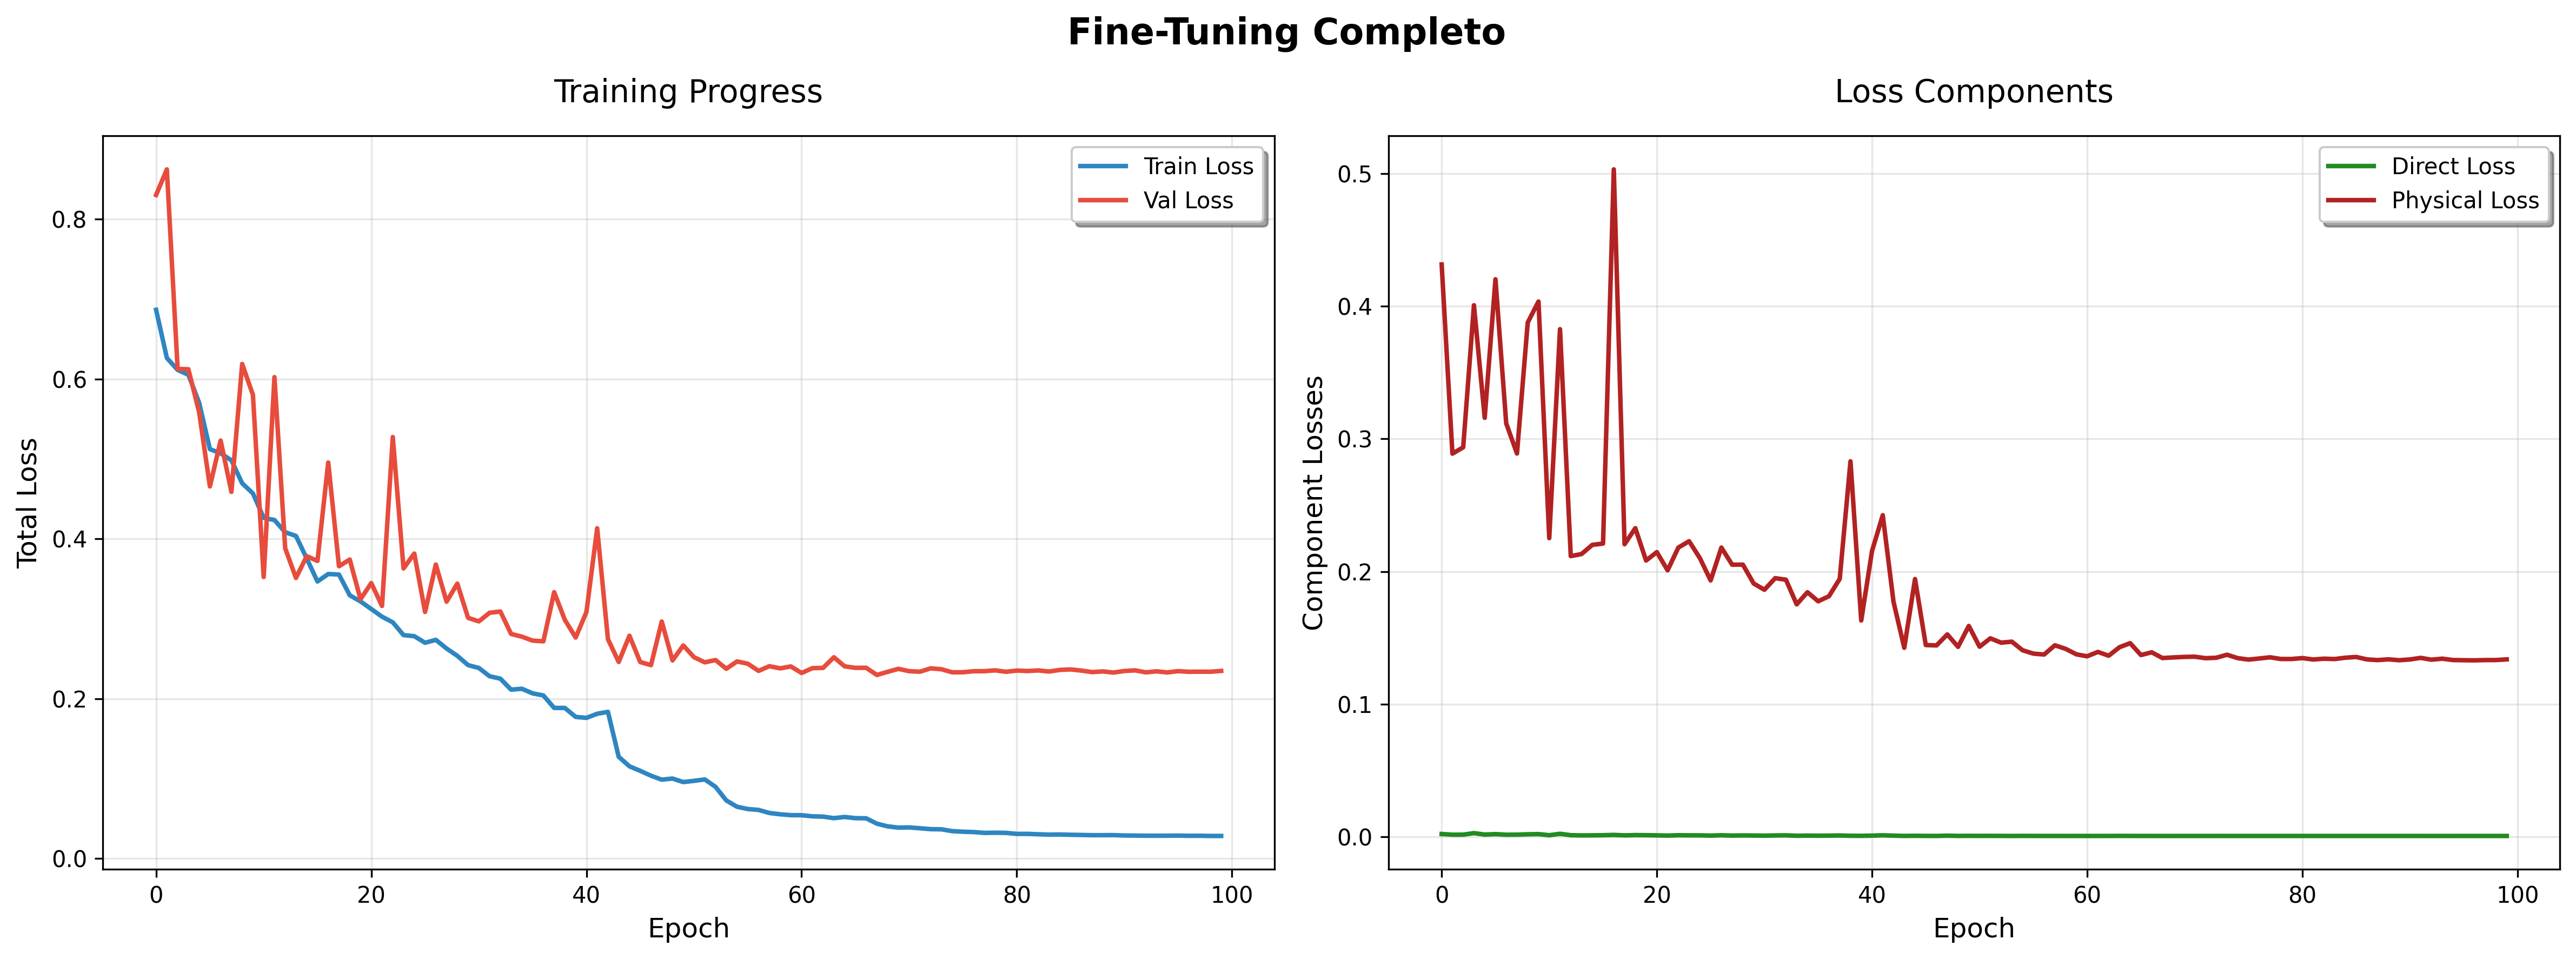
\includegraphics[width=0.8\textwidth]{Images/perdidas_entrenamiento_finetuning.png}
    \caption{Evolución de la función de pérdida durante el fine-tuning de la red reconstructora.}
    \label{fig:reconstructor_finetuning}
\end{figure}

La gráfica de evolución de pérdidas durante el fine-tuning muestra dos componentes principales: la pérdida directa (reconstrucción) y la pérdida física. La pérdida directa, heredada del preentrenamiento del reconstructor U-Net, se mantiene consistentemente baja (cercana a 0.005) durante todo el proceso, indicando que la red mantiene su capacidad de reconstrucción de imágenes.
La pérdida física, por otro lado, inicia con valores altos (~0.4-0.5) y muestra alta volatilidad en las primeras 20 épocas. Posteriormente, se estabiliza gradualmente hasta converger alrededor de 0.13. Esta evolución sugiere que la red está aprendiendo progresivamente a satisfacer las restricciones físicas sin comprometer significativamente su capacidad de reconstrucción original.
La curva de pérdida total muestra una brecha entre entrenamiento y validación similar a lo observado en el supervisor, con el entrenamiento convergiendo a ~0.05 y la validación a ~0.2, lo cual es esperado dado el componente físico añadido.


\subsubsection{Ablación de componentes de la función de pérdida} \label{subsec:ablation}

Como bien esta descrito en la sección \ref{subsubsec:pretraining}, la función de pérdida propuesta consta de cuatro componentes: pérdida directa, pérdida física, pérdida estructural y pérdida de similitud, donde la pérdida estructural tiene un gran peso sobre los demás componentes. Para evaluar la importancia de cada componente en la función de pérdida, se realizaron experimentos de ablación eliminando cada componente de la función de pérdida mientras se mantenían los demás términos constantes. Los resultados obtenidos durante el fine-tuning de la red constructora se muestran en la Figura \ref{fig:ablation_no_struct} y \ref{fig:ablation_no_phys}.

\begin{figure}[H]
    \centering
    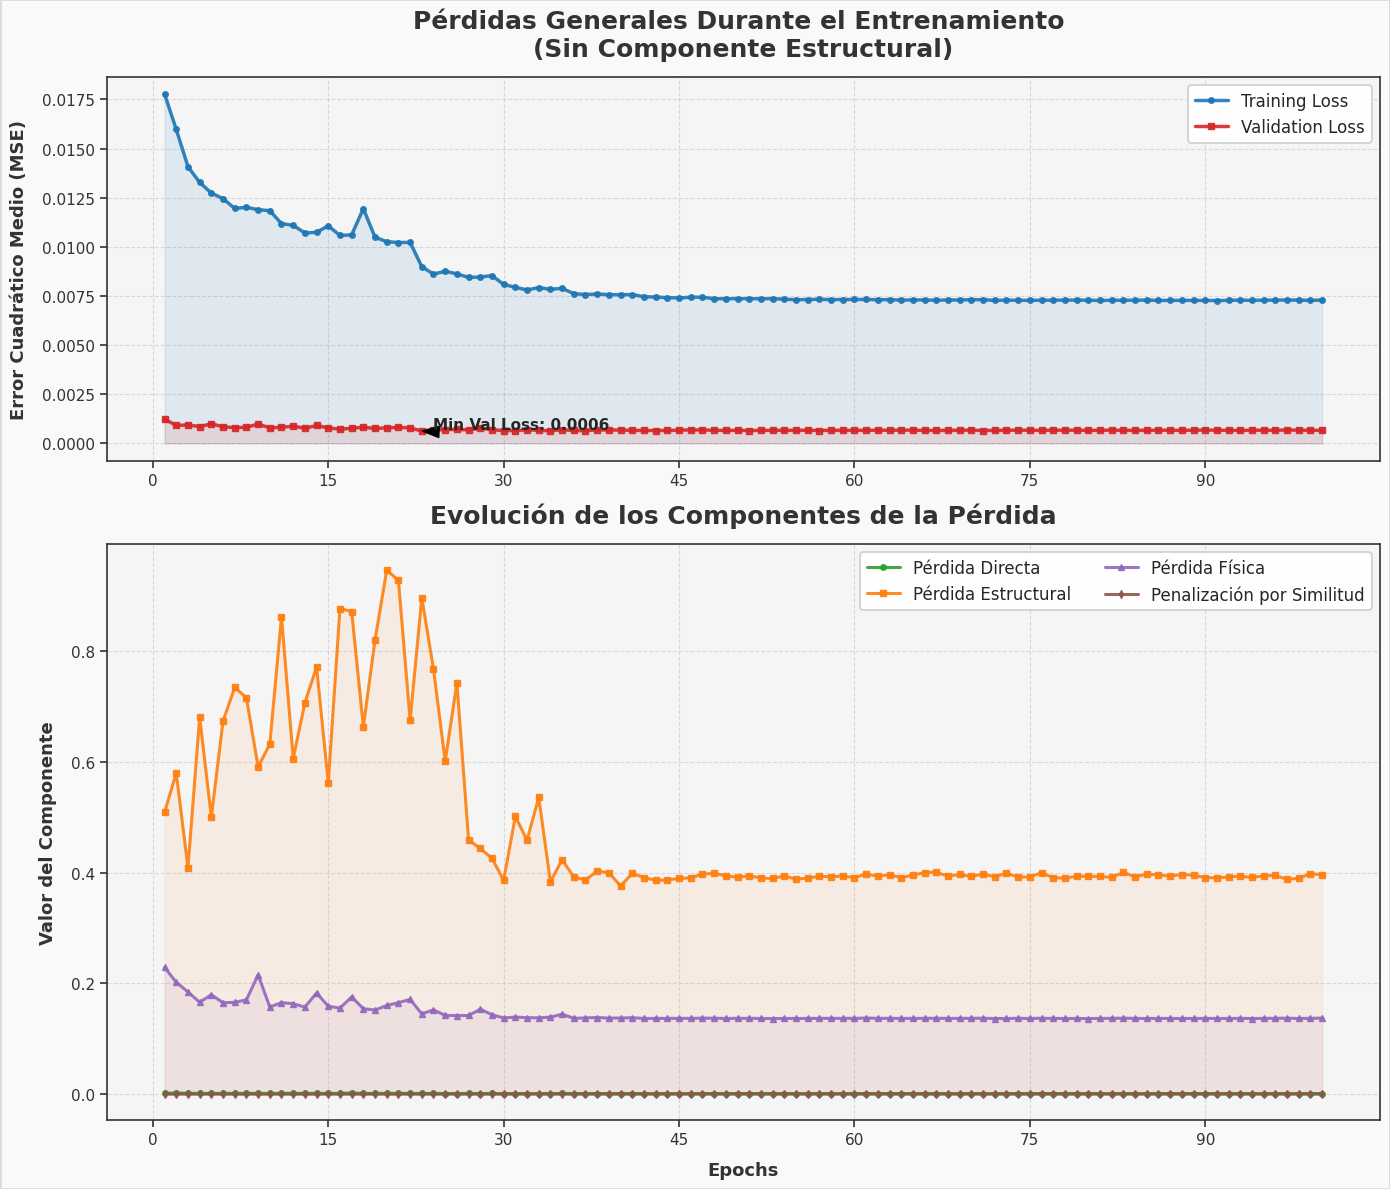
\includegraphics[width=0.8\textwidth]{Images/perdidas_entrenamiento_finetuning_no_struct.png}
    \caption{Evolución de la función de pérdida durante el fine-tuning de la red constructora eliminando la pérdida estructural.}
    \label{fig:ablation_no_struct}
\end{figure}

\begin{figure}[H]
    \centering
    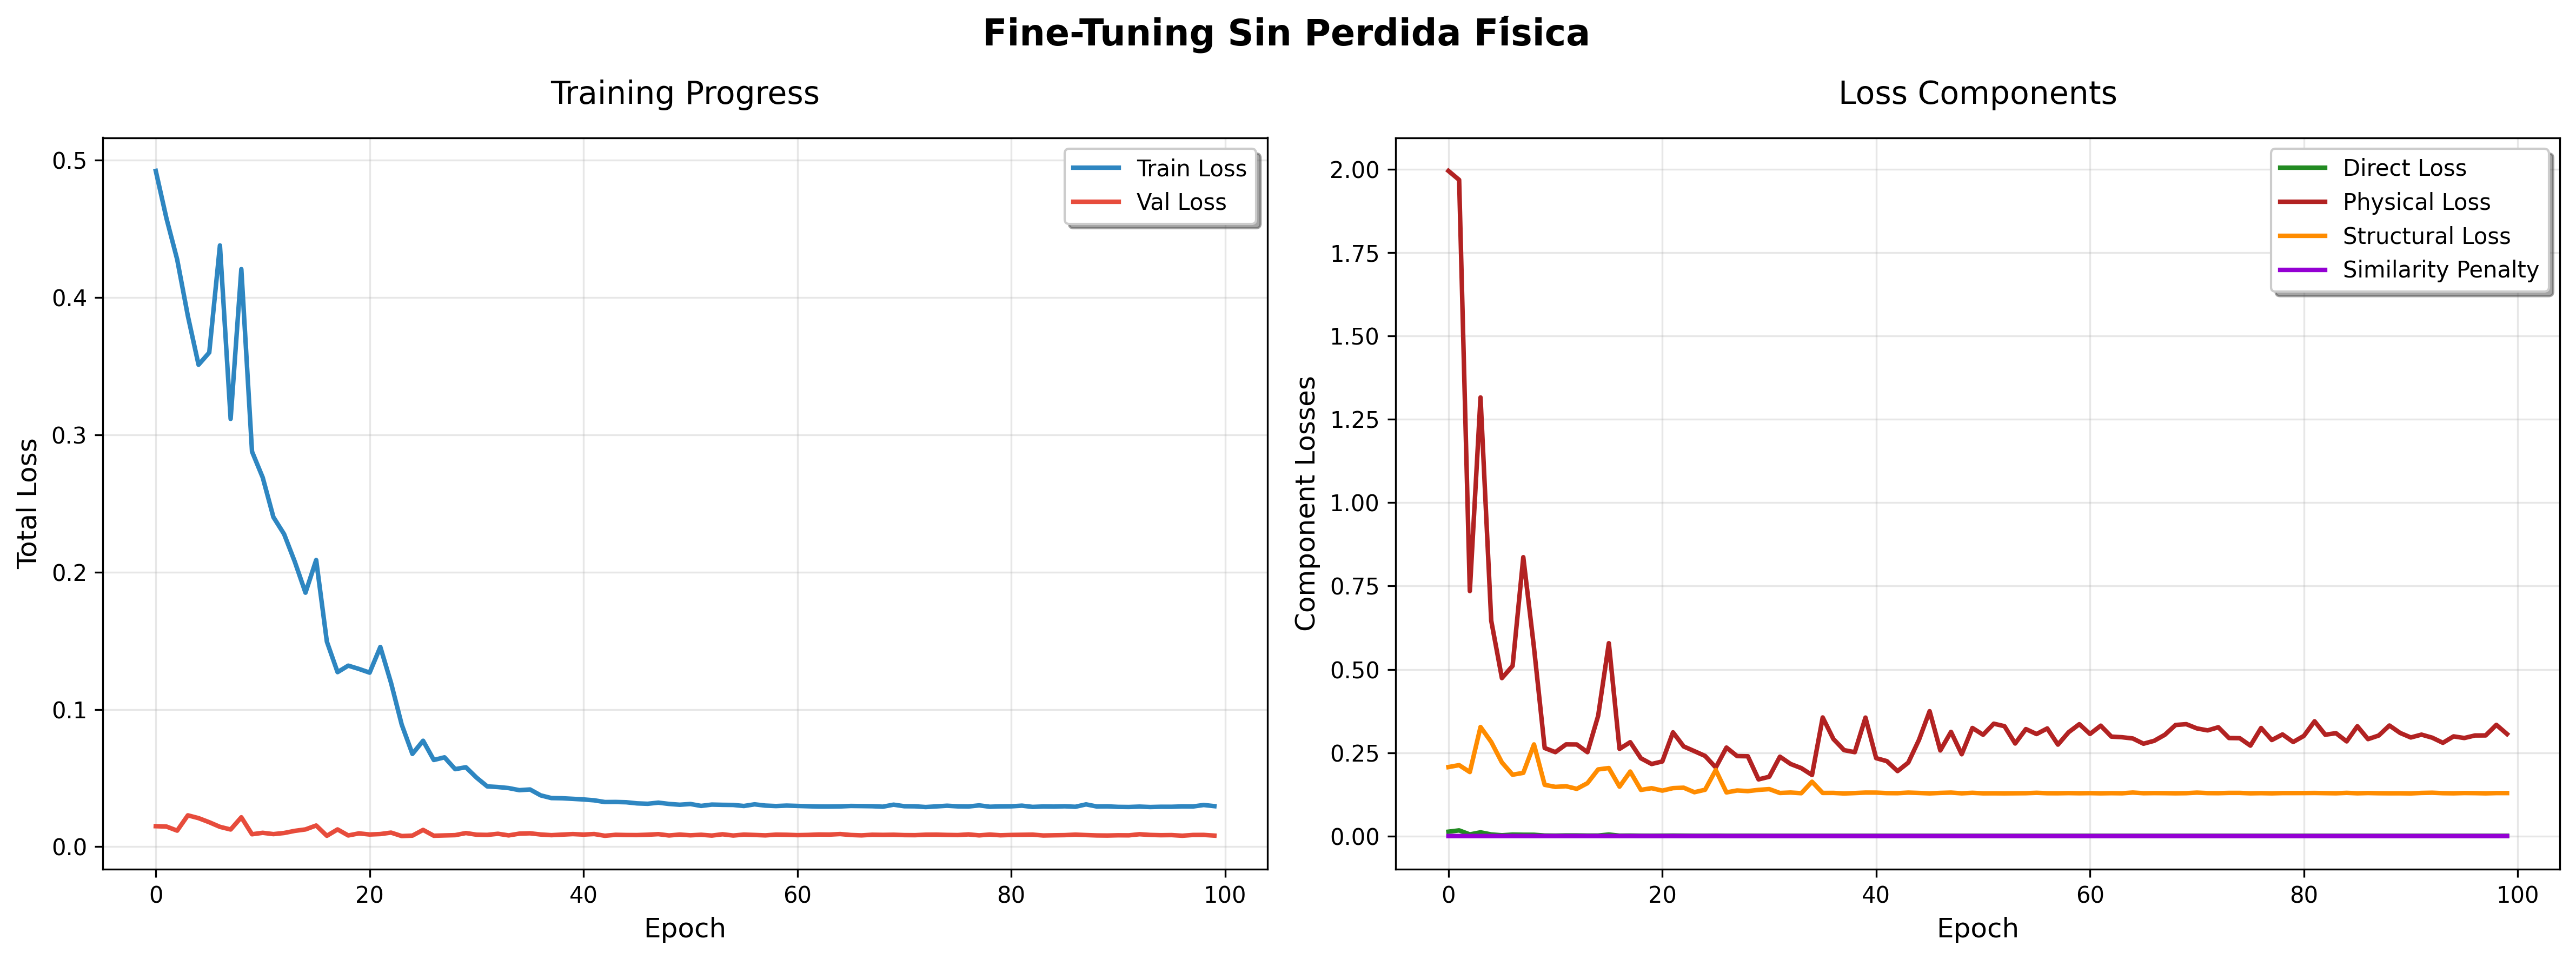
\includegraphics[width=0.8\textwidth]{Images/perdidas_entrenamiento_finetuning_no_phy.png}
    \caption{Evolución de la función de pérdida durante el fine-tuning de la red constructora eliminando la pérdida física.}
    \label{fig:ablation_no_phys}
\end{figure}

El análisis de las gráficas de fine-tuning revela comportamientos distintivos al eliminar diferentes componentes de pérdida. En el caso sin pérdida estructural, observamos una pérdida total inicial de aproximadamente 0.5 que converge gradualmente a 0.03. La pérdida física muestra una dinámica particularmente interesante, comenzando en valores cercanos a 2.0 con oscilaciones pronunciadas en las primeras 20 épocas, antes de estabilizarse alrededor de 0.3. Las pérdidas directa y de similitud se mantienen consistentemente cercanas a cero, aunque se observa una brecha notable entre las curvas de entrenamiento y validación.

Por otro lado, cuando se elimina la pérdida física, el comportamiento del modelo cambia significativamente. La pérdida total se mantiene en un rango mucho menor, iniciando en aproximadamente 0.0175. La pérdida estructural se convierte en el componente dominante, mostrando un patrón distintivo donde aumenta inicialmente hasta alcanzar un pico de 0.8 alrededor de la época 20, para luego estabilizarse en aproximadamente 0.4. Es notable que la pérdida directa y la pérdida de similitud se mantienen excepcionalmente bajas (~0.001), sugiriendo que el modelo preserva su capacidad de reconstrucción básica. La convergencia en este caso es más suave y estable en comparación con el escenario sin pérdida estructural, indicando una optimización más consistente del modelo.

\subsection{Metricas de evaluación}

Para evaluar la calidad de las imágenes generadas por la red reconstructora, se utilizaron las métricas de evaluación descritas en la sección \ref{sec:metrics}. Las métricas de evaluación se calcularon para las imágenes generadas por la red reconstructora en el conjunto de prueba. Los resultados obtenidos se muestran en la Tabla \ref{tab:metricas}.

\begin{table}[H]
    \centering
    \begin{tabularx}{\textwidth}{lXXXXXX}
    \hline
    \textbf{Modelo} & \textbf{MSE} & \textbf{MAE} & \textbf{NRMSE} & \textbf{PSNR} (dB) & \textbf{SSIM} \\
    \hline
    Baseline & $9\times10^{-3} \pm 0.0005$ & $3\times10^{-2} \pm 0.002$ & $4\times10^{-1} \pm 0.01$ & $29.0 \pm 2.0$ & $0.96 \pm 0.01$ \\
    FT & $7\times10^{-3} \pm 0.0006$ & $2\times10^{-2} \pm 0.002$ & $3\times10^{-1} \pm 0.03$ & $30.0 \pm 3.0$ & $0.97 \pm 0.01$ \\
    FT No-Physical & $1\times10^{-2} \pm 0.0008$ & $4\times10^{-2} \pm 0.003$ & $4\times10^{-1} \pm 0.03$ & $28.0 \pm 3.0$ & $0.95 \pm 0.01$ \\
    FT No-Structural & $1\times10^{-2} \pm 0.001$ & $1\times10^{-1} \pm 0.001$ & $4\times10^{-1} \pm 0.04$ & $27.0 \pm 2.0$ & $0.62 \pm 0.1$ \\
    \hline
    \end{tabularx}
    \caption{Métricas de evaluación de las imágenes generadas por la red reconstructora en el conjunto de prueba. Los valores incluyen las desviaciones estándar.}
    \label{tab:metricas}
\end{table}

En las siguientes secciones se profundiza en cada una de estas metricas y se comparan los resultados obtenidos con la metodología propuesta con los obtenidos al entrenar solo la U-Net. Además, se evalúa la importancia de cada componente de la función de pérdida propuesta al eliminarlo del finetuning.

\subsubsection{Error Absoluto Medio (MAE)}

El Error Absoluto Medio (MAE) proporciona una medida directa de la magnitud promedio de los errores de reconstrucción. La Figura \ref{fig:mae_analysis} presenta un análisis comparativo entre el modelo pre-entrenado y las tres variantes de fine-tuning implementadas.

\begin{figure}[H]
    \centering
    \begin{subfigure}[b]{0.48\textwidth}
        \centering
        % FT No-Physical vs Baseline
        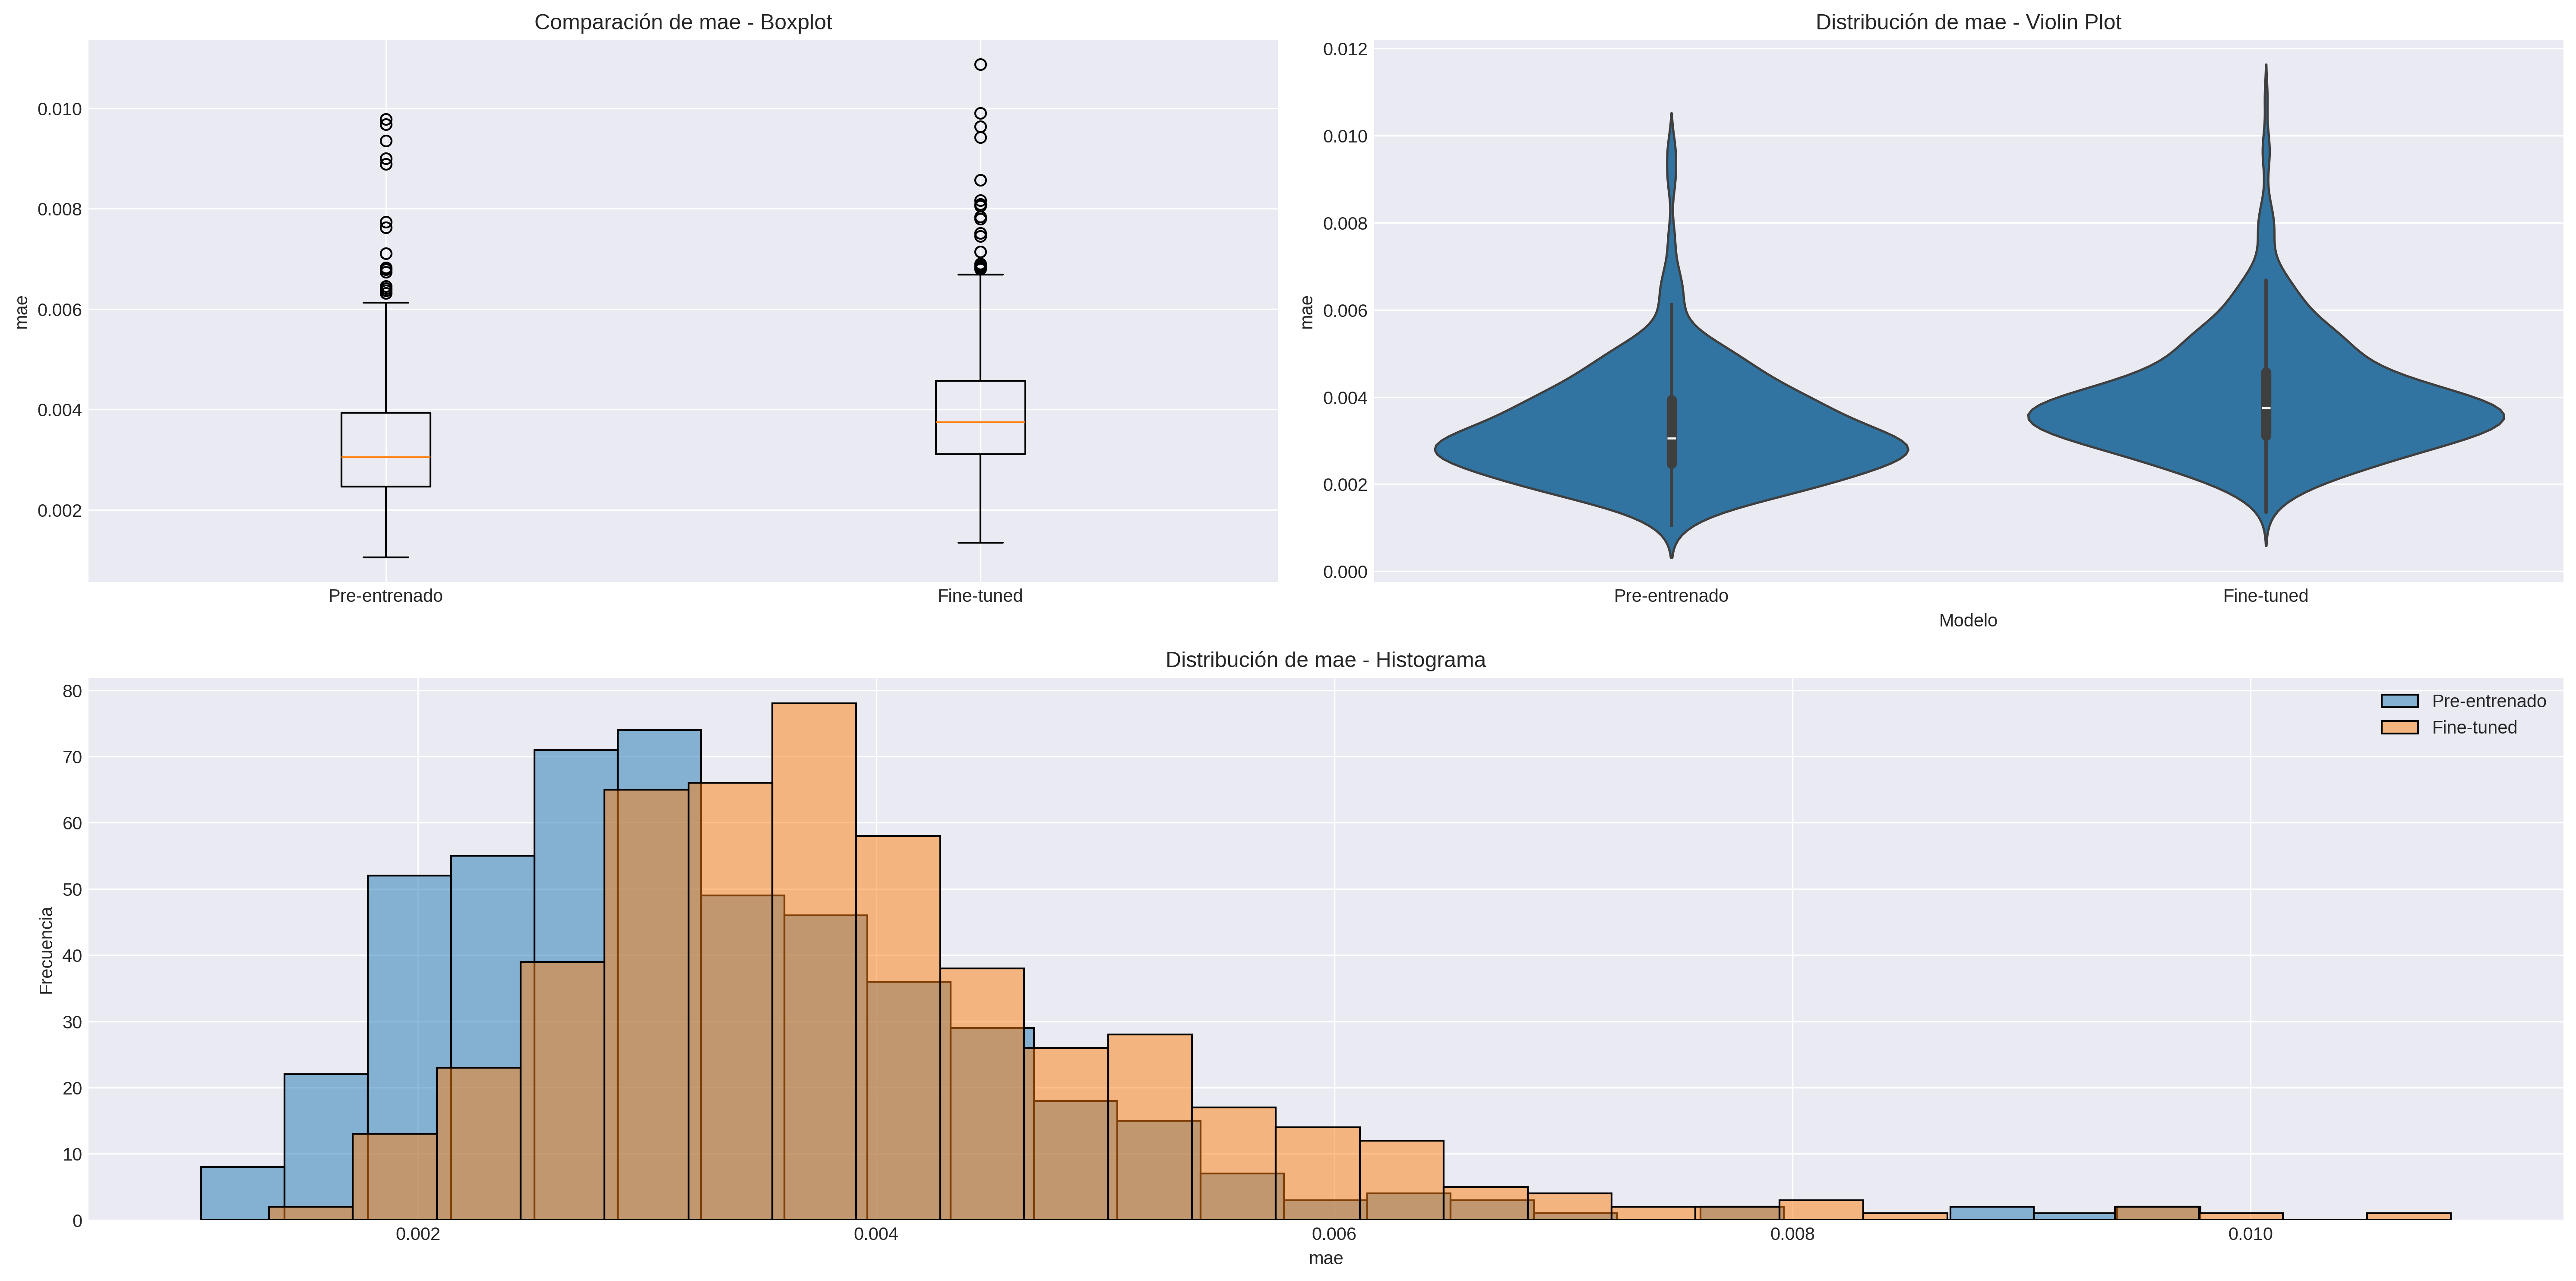
\includegraphics[width=\textwidth]{Images/comparison_plots_mae_no_phy.png}
        \caption{Comparación entre fine-tuning sin componente física y modelo pre-entrenado}
        \label{fig:mae_hist}
    \end{subfigure}
    \hfill
    \begin{subfigure}[b]{0.48\textwidth}
        \centering
        % FT No-Structural vs Baseline
        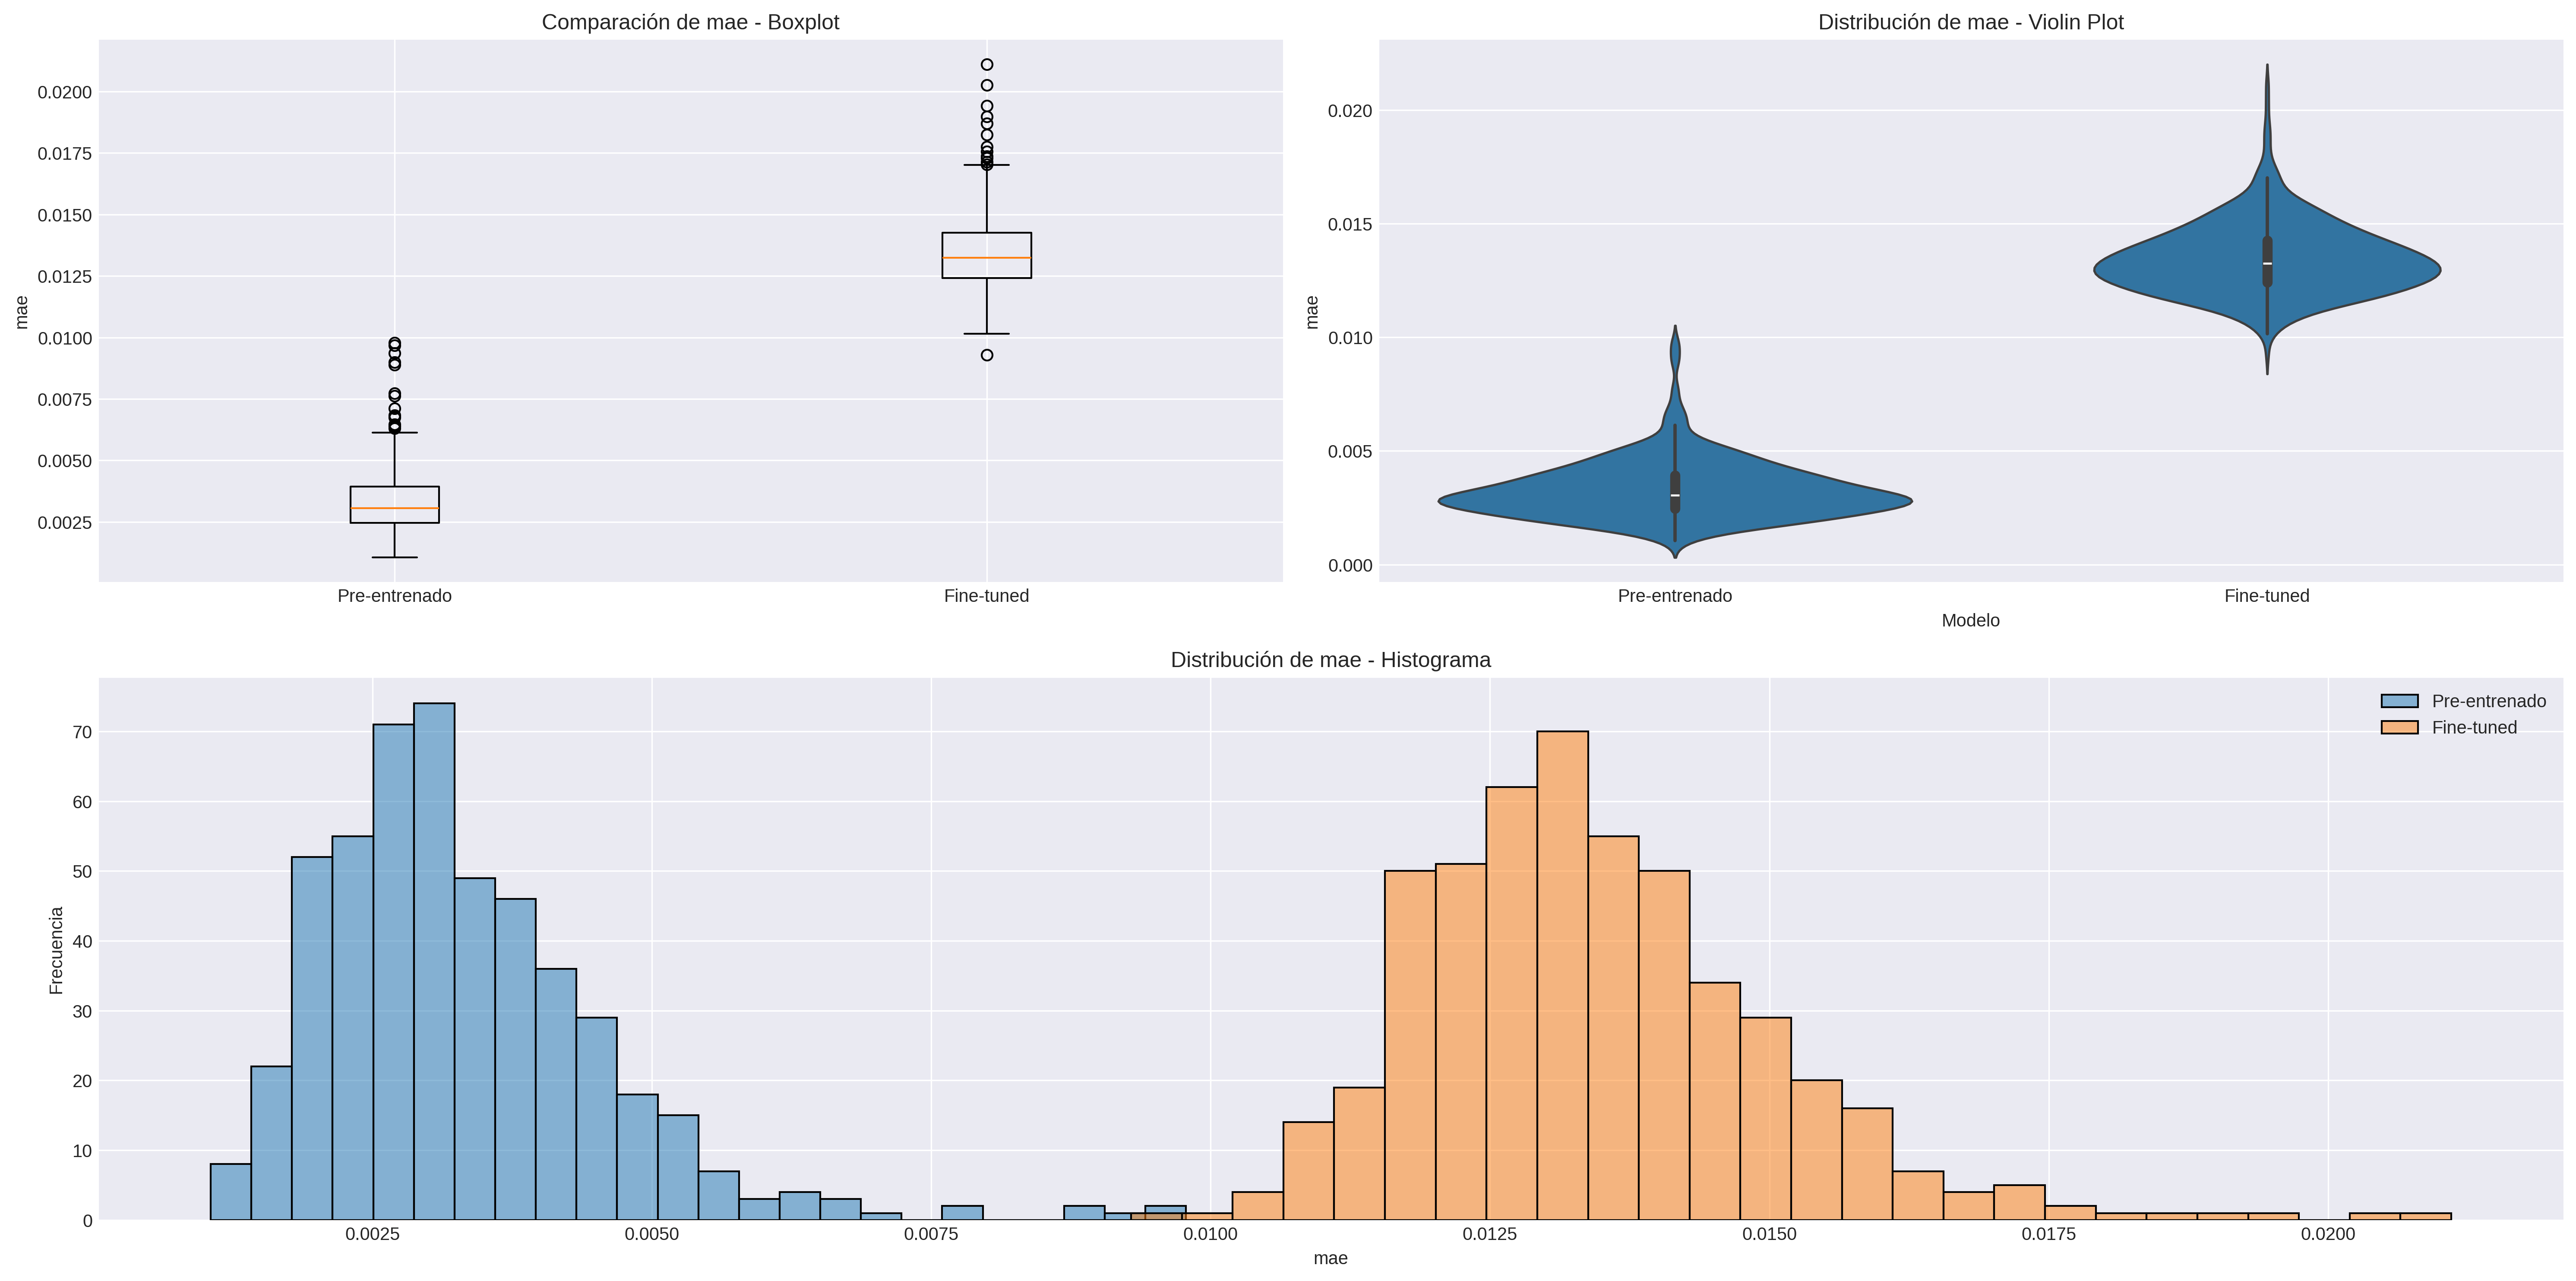
\includegraphics[width=\textwidth]{Images/comparison_plots_mae_no_struct.png}
        \caption{Comparación entre fine-tuning sin componente estructural y modelo pre-entrenado}
        \label{fig:mae_violin}
    \end{subfigure}
    
    \vspace{0.5cm}
    
    \begin{subfigure}[b]{0.7\textwidth}
        \centering
        % FT vs Baseline
        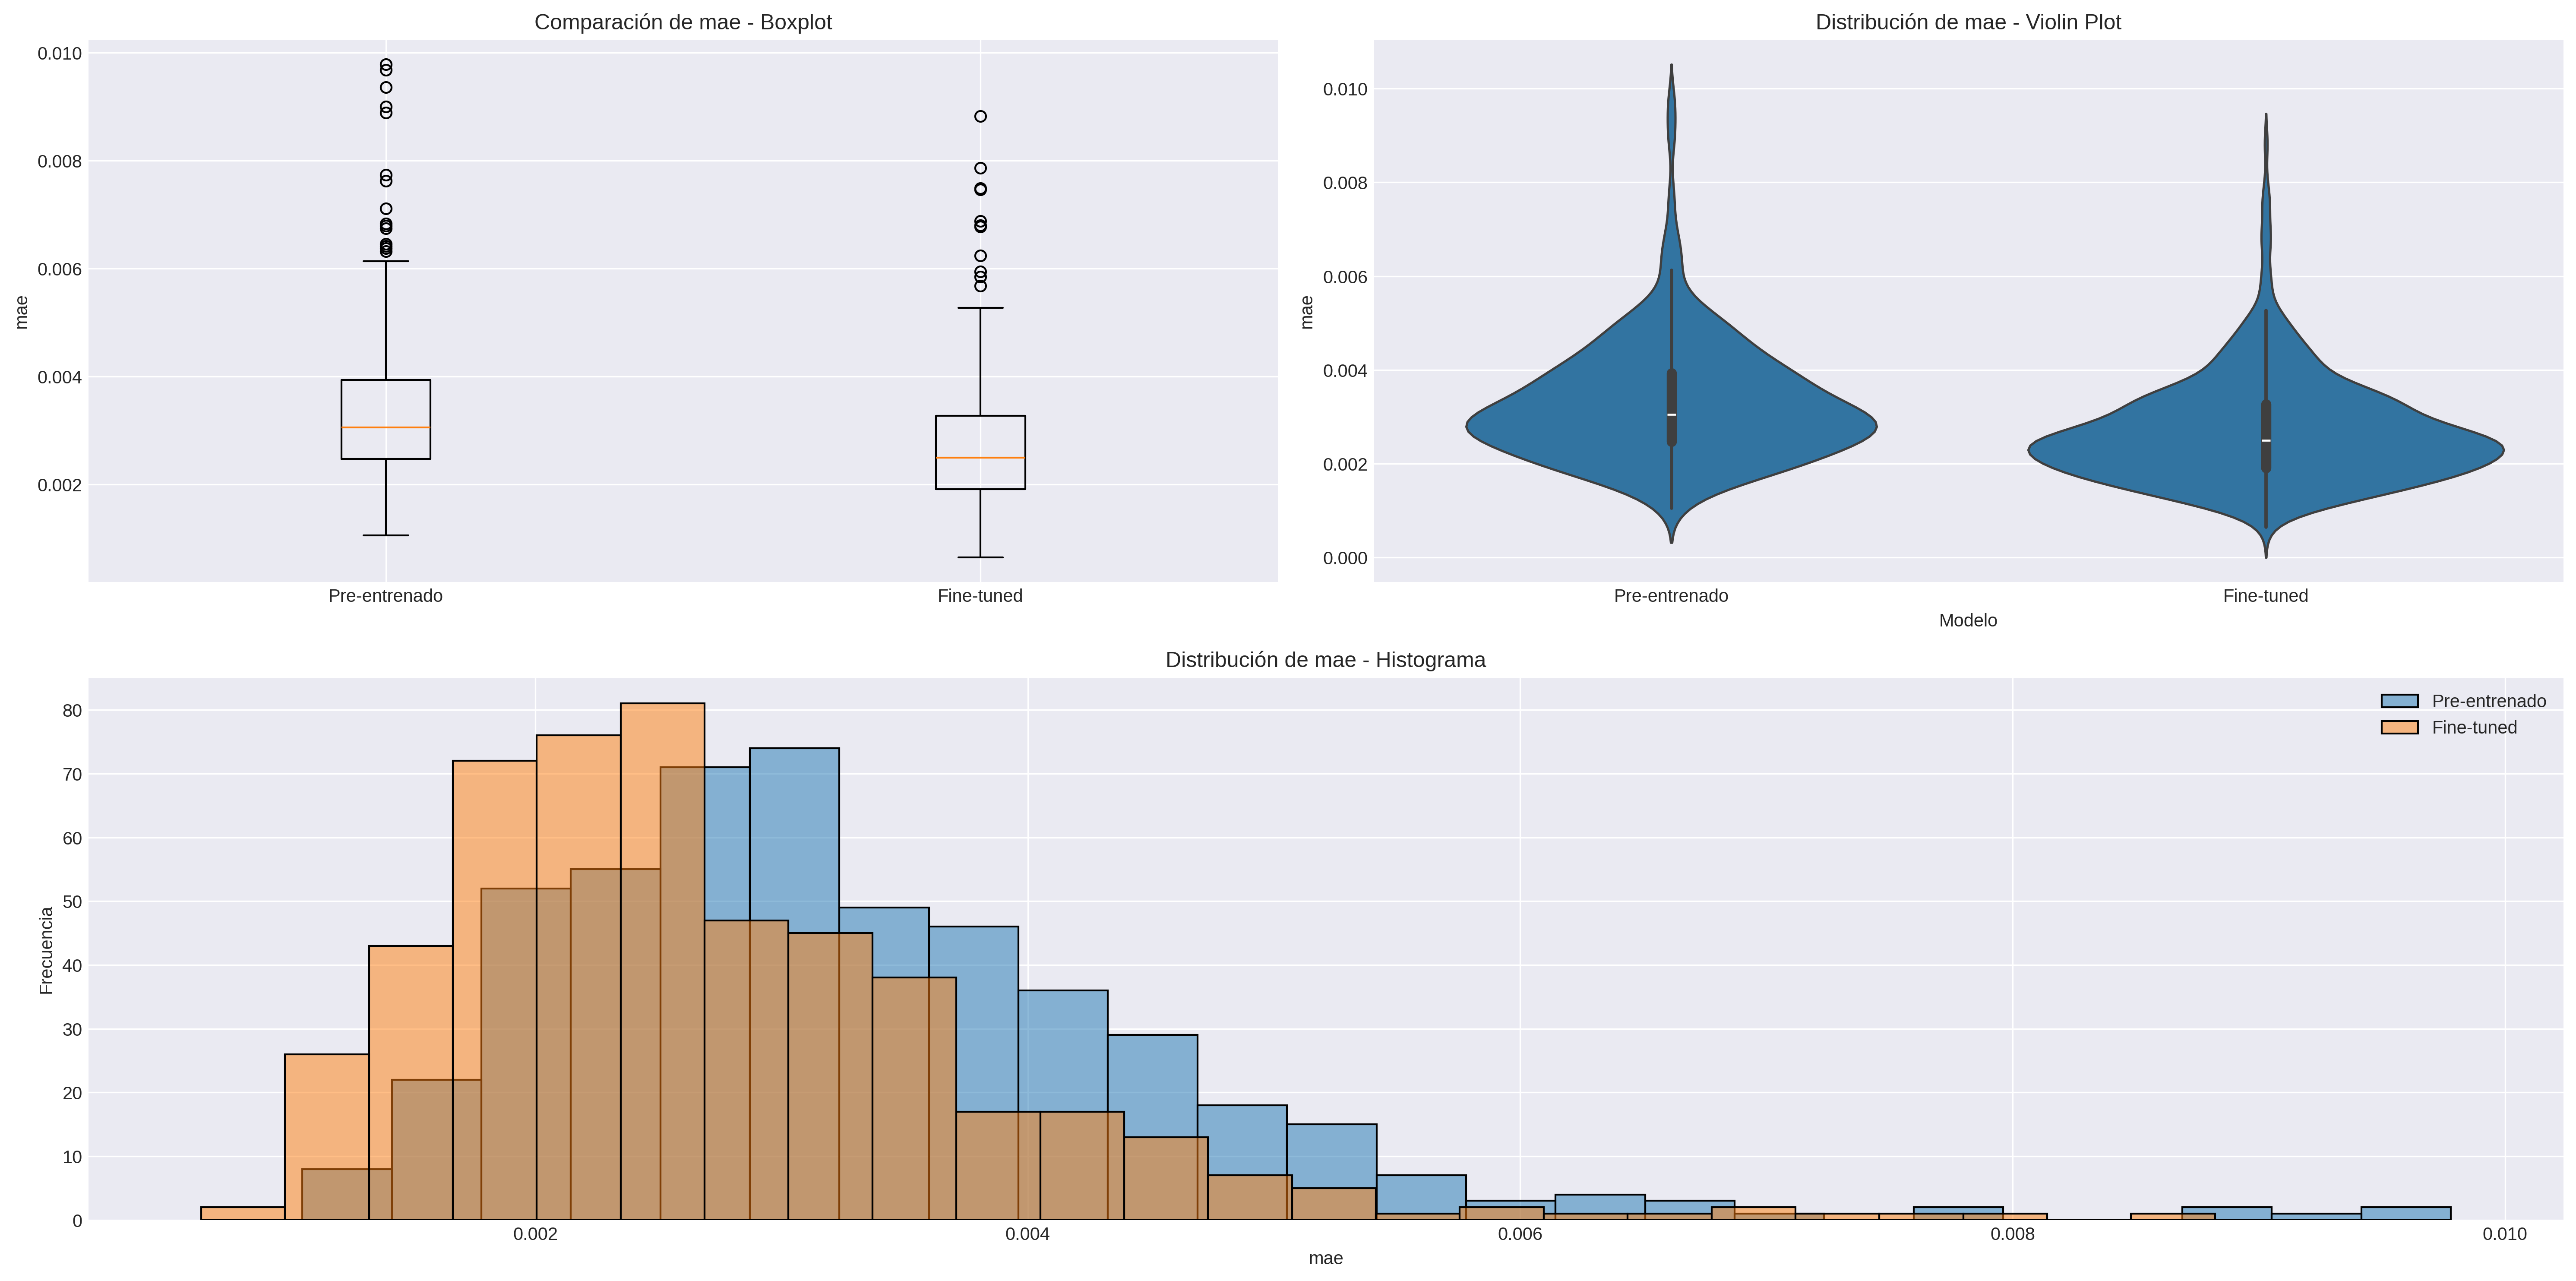
\includegraphics[width=\textwidth]{Images/comparison_plots_mae_sup.png}
        \caption{Comparación entre fine-tuning (FT) completo y modelo pre-entrenado}
        \label{fig:mae_box}
    \end{subfigure}
    
    \caption{Análisis comparativo del Error Absoluto Medio (MAE) entre el modelo pre-entrenado y las variantes de fine-tuning implementadas. a) Comparación entre fine-tuning sin componente física y modelo pre-entrenado. b) Comparación entre fine-tuning sin componente estructural y modelo pre-entrenado. c) Comparación entre fine-tuning completo y modelo pre-entrenado.}
    \label{fig:mae_analysis}
\end{figure}


\paragraph{Fine-tuning Completo (FT)}
El modelo con fine-tuning completo demuestra una mejora significativa en el rendimiento respecto al modelo pre-entrenado. El MAE medio se redujo de $3.301 \times 10^{-3}$ (pre-entrenado) a $2.690 \times 10^{-3}$ (fine-tuned), representando una mejora del 18.50\%. La dispersión de los errores también se redujo, como lo evidencia la disminución en la desviación estándar de $1.276 \times 10^{-3}$ a $1.114 \times 10^{-3}$. El rango de errores se contrajo, con el valor mínimo mejorando de $1.054 \times 10^{-3}$ a $0.643 \times 10^{-3}$ y el máximo reduciéndose de $9.780 \times 10^{-3}$ a $8.822 \times 10^{-3}$.

La significancia estadística de esta mejora se confirma mediante múltiples pruebas. Aunque las pruebas de Shapiro-Wilk ($W = 0.9027$ y $W = 0.9006$, ambas con $p < 0.001$) indican que las distribuciones no son normales, tanto la prueba t pareada ($t = 19.6755$, $p < 0.001$) como la prueba no paramétrica de Wilcoxon ($W = 10619.0000, p < 0.001$) confirman que la diferencia es estadísticamente significativa. El tamaño del efecto ($d$ de $Cohen = 0.5099$) indica una mejora prácticamente significativa de magnitud media a grande.

\paragraph{Fine-tuning sin Componente Física (FT No-Physical)}
La eliminación de la componente física en el fine-tuning resulta en un deterioro significativo del rendimiento. El MAE medio aumentó a $3.975 \times 10^{-3}$, representando un incremento del 20.42\% respecto al modelo pre-entrenado ($3.301 \times 10^{-3}$). La variabilidad de los errores también aumentó, con una desviación estándar de $1.321 \times 10^{-3}$. El rango de errores se expandió, con un valor mínimo de $1.349 \times 10^{-3}$ y un máximo de $10.873 \times 10^{-3}$.

Las pruebas estadísticas confirman el impacto negativo de eliminar la componente física. La prueba t pareada ($t = -27.5056$, $p < 0.001$) y la prueba de Wilcoxon ($W = 4313.0000$, $p < 0.001$) indican que el deterioro es estadísticamente significativo. El tamaño del efecto negativo ($d$ de $Cohen = -0.5192$) sugiere que la ausencia de la componente física tiene un impacto sustancial en el rendimiento del modelo.

\paragraph{Fine-tuning sin Componente Estructural (FT No-Structural)}
La ausencia de la componente estructural produce el deterioro más severo en el rendimiento del modelo. El MAE medio se incrementó dramáticamente a $13.438 \times 10^{-3}$, representando un empeoramiento del 307.08\% respecto al modelo pre-entrenado. La dispersión de los errores aumentó significativamente, con una desviación estándar de $1.559 \times 10^{-3}$. El rango de errores se expandió considerablemente, con un valor mínimo de $9.289 \times 10^{-3}$ y un máximo de $21.101 \times 10^{-3}$.

El análisis estadístico revela la magnitud del impacto negativo. Las pruebas de significancia muestran diferencias extremadamente significativas, con un estadístico $t$ de $-269.9921$ ($p < 0.001$) y un estadístico de Wilcoxon $W = 0 (p < 0.001)$. El tamaño del efecto es notablemente grande y negativo ($d$ de $Cohen = -7.1154$), indicando que la componente estructural es crucial para el rendimiento del modelo. Esta degradación sustancial en el rendimiento subraya la importancia fundamental de la componente estructural en la función de pérdida.

\subsubsection{Error Cuadrático Medio (MSE)}

El Error Cuadrático Medio (MSE) proporciona una medida cuantitativa de la magnitud promedio de los errores de reconstrucción. La Figura \ref{fig:mse_analysis} presenta un análisis comparativo entre el modelo pre-entrenado y las tres variantes de fine-tuning implementadas.

\begin{figure}
    \begin{figure}[H]
        \centering
        \begin{subfigure}[b]{0.48\textwidth}
            \centering
            % FT No-Physical vs Baseline
            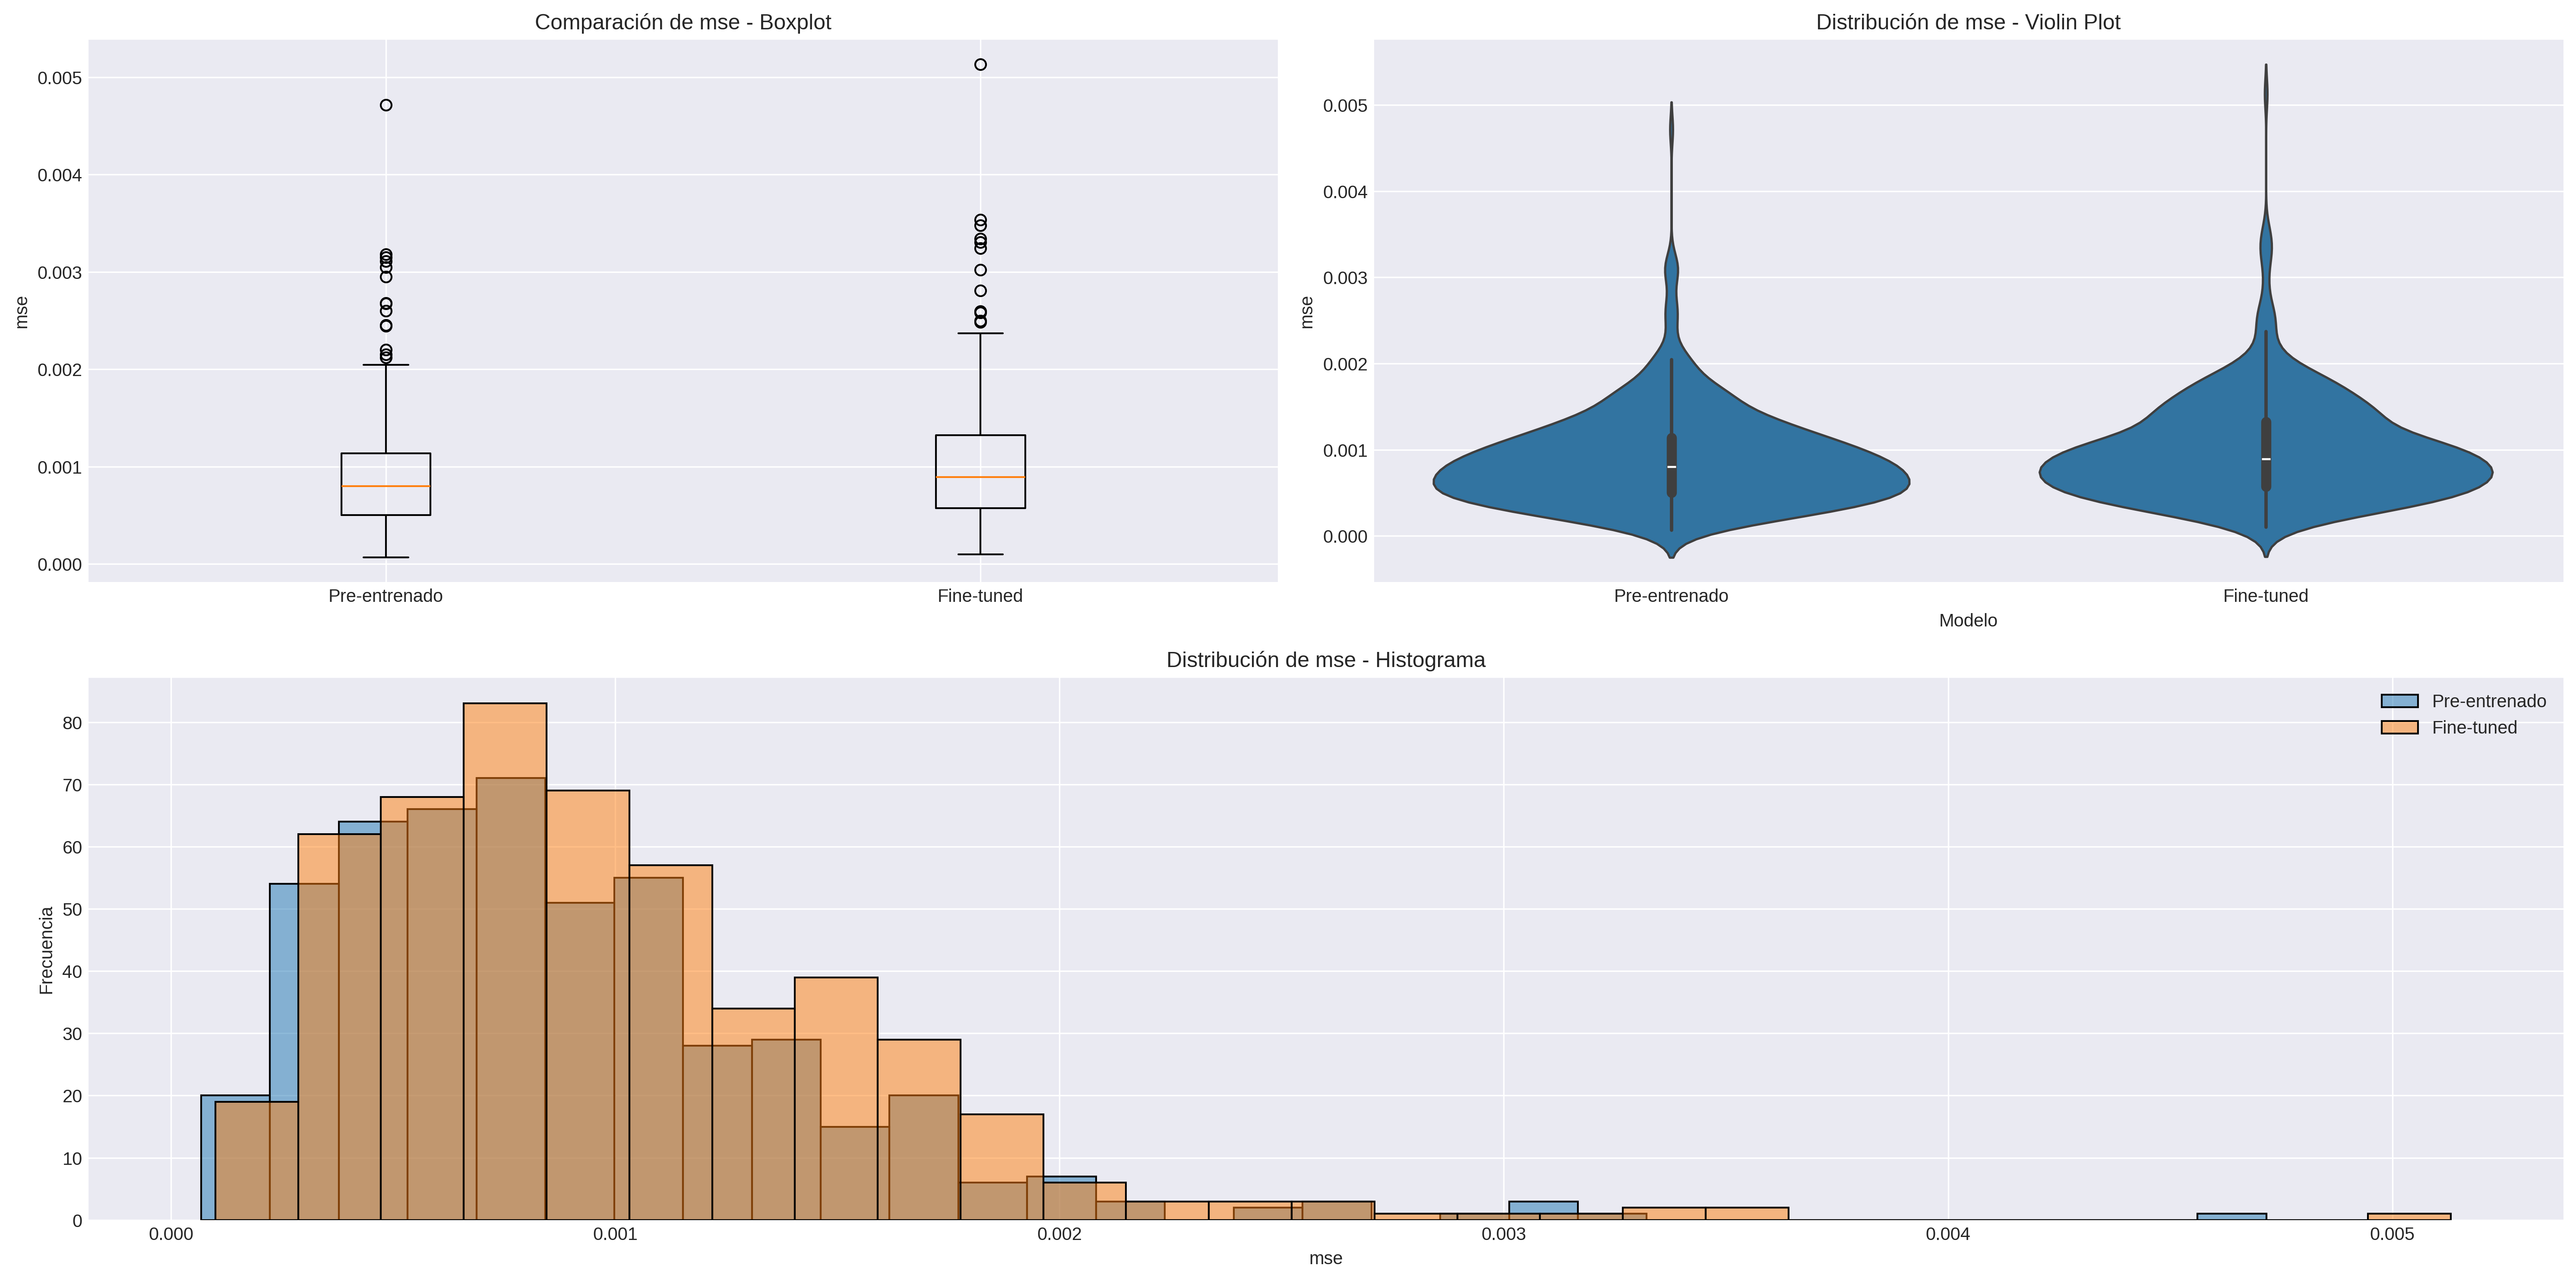
\includegraphics[width=\textwidth]{Images/comparison_plots_mse_no_phy.png}
            \caption{Comparación entre fine-tuning sin componente física y modelo pre-entrenado}
            \label{fig:mse_completo}
        \end{subfigure}
        \hfill
        \begin{subfigure}[b]{0.48\textwidth}
            \centering
            % FT No-Structural vs Baseline
            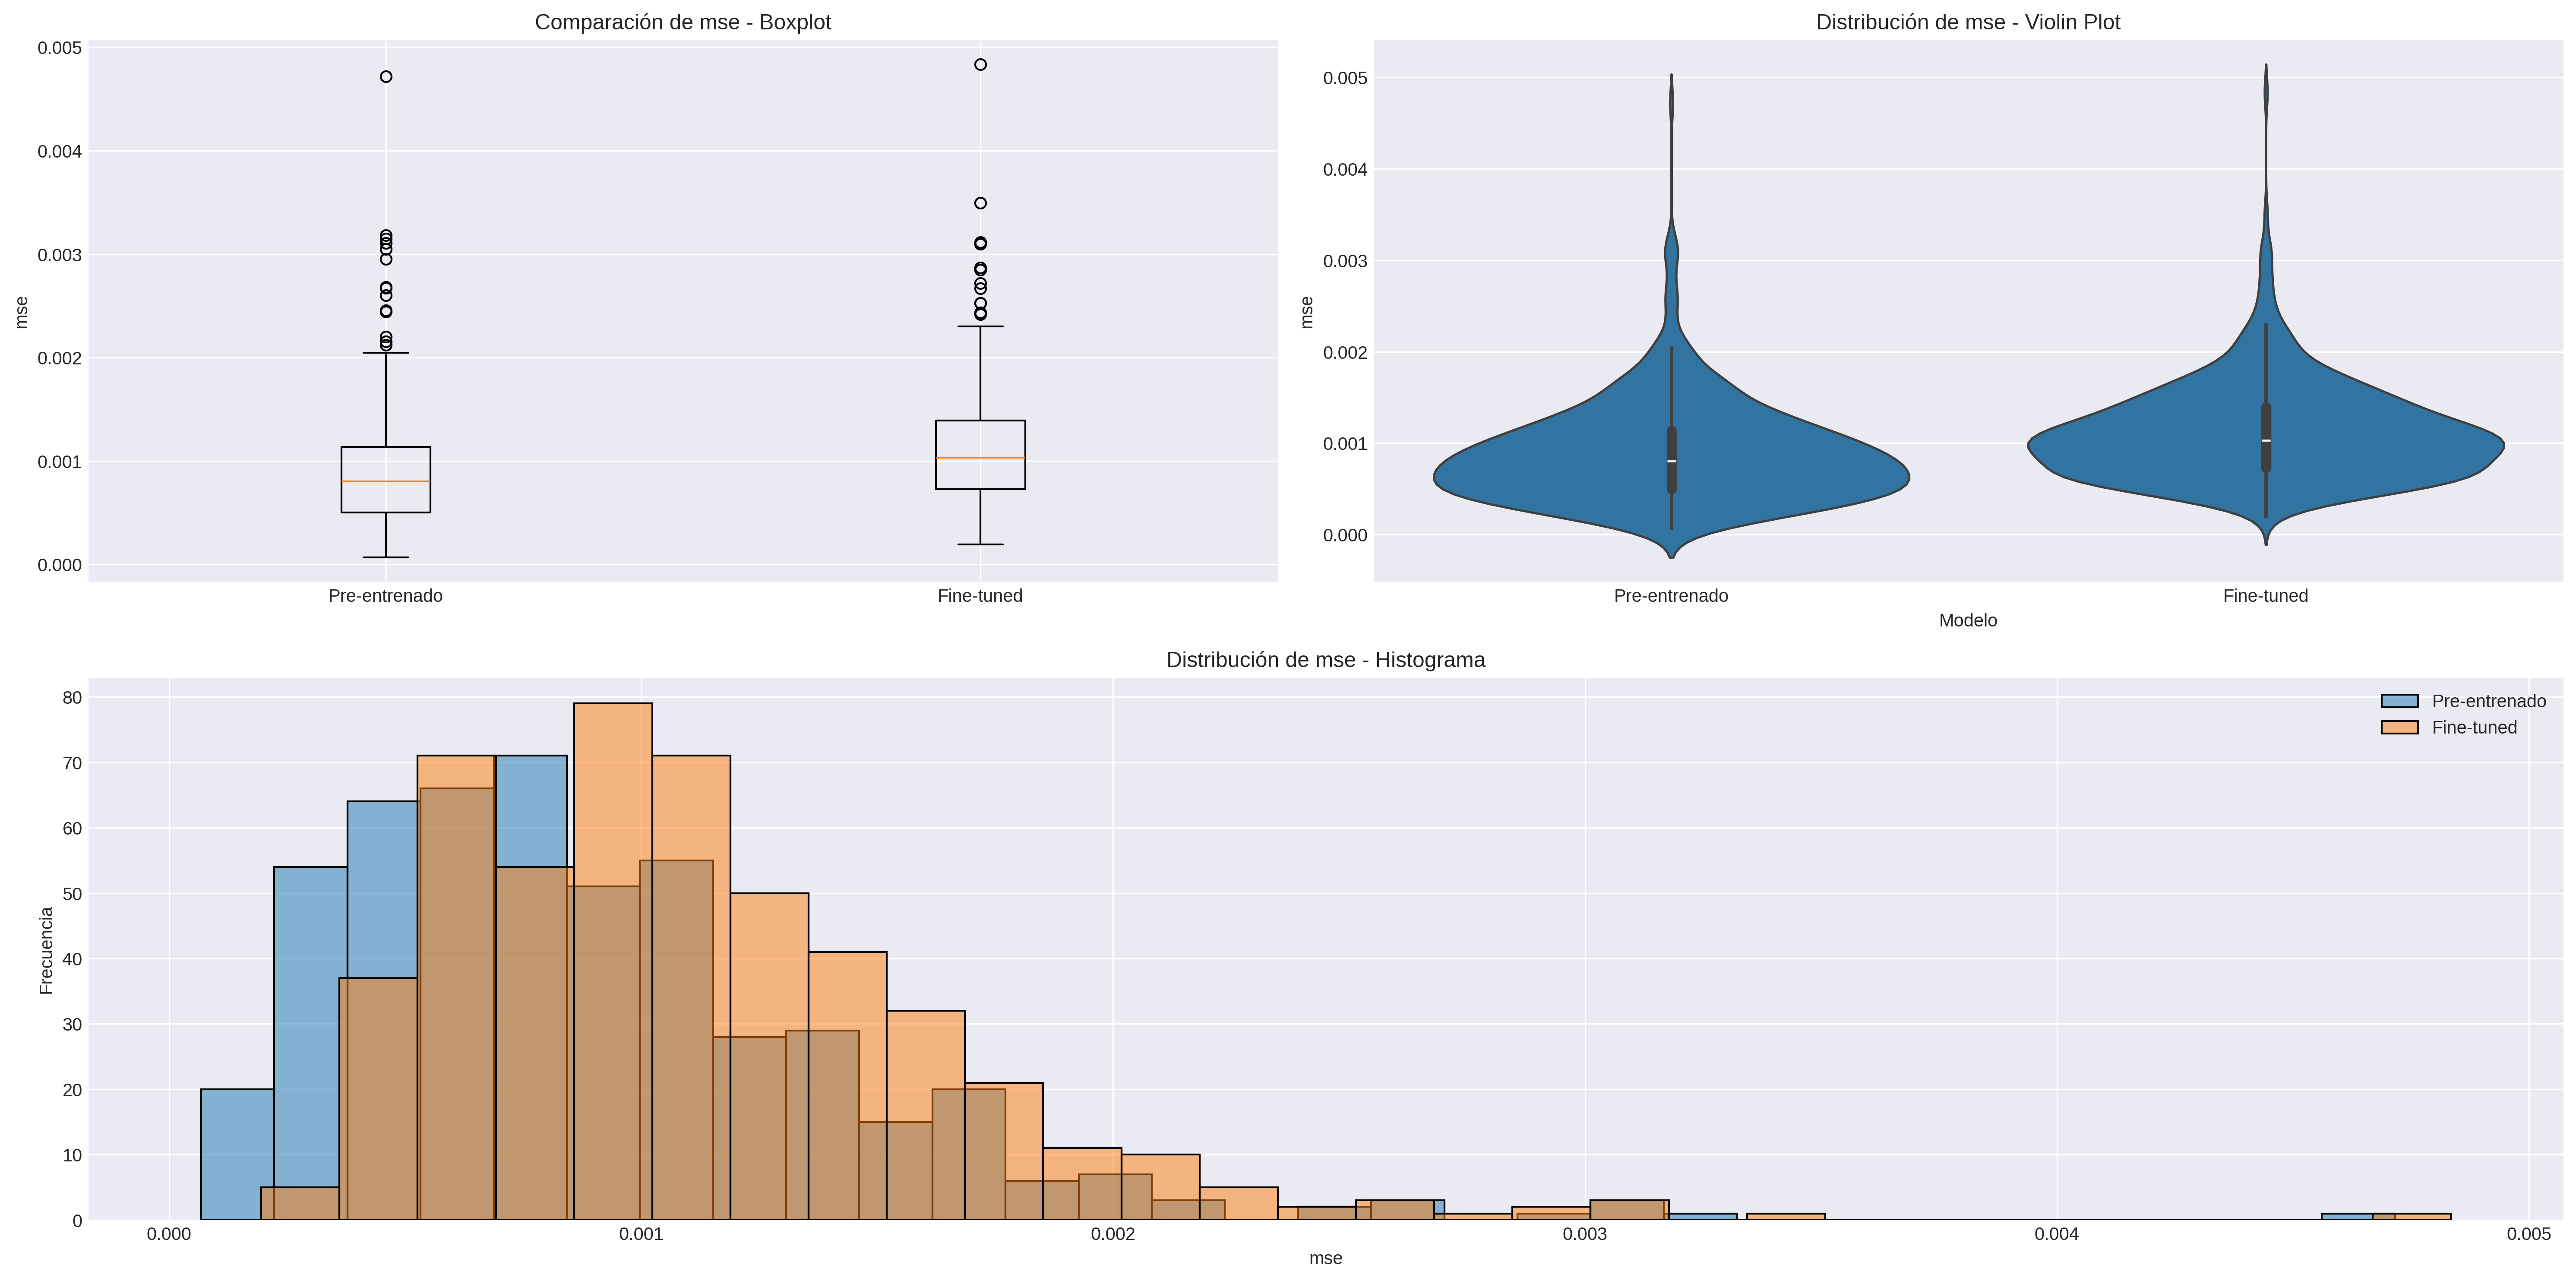
\includegraphics[width=\textwidth]{Images/comparison_plots_mse_no_struct.png}
            \caption{Comparación entre fine-tuning sin componente estructural y modelo pre-entrenado}
            \label{fig:mse_no_struct}
        \end{subfigure}
        
        \vspace{0.5cm}
        
        \begin{subfigure}[b]{0.7\textwidth}
            \centering
            % FT vs Baseline
            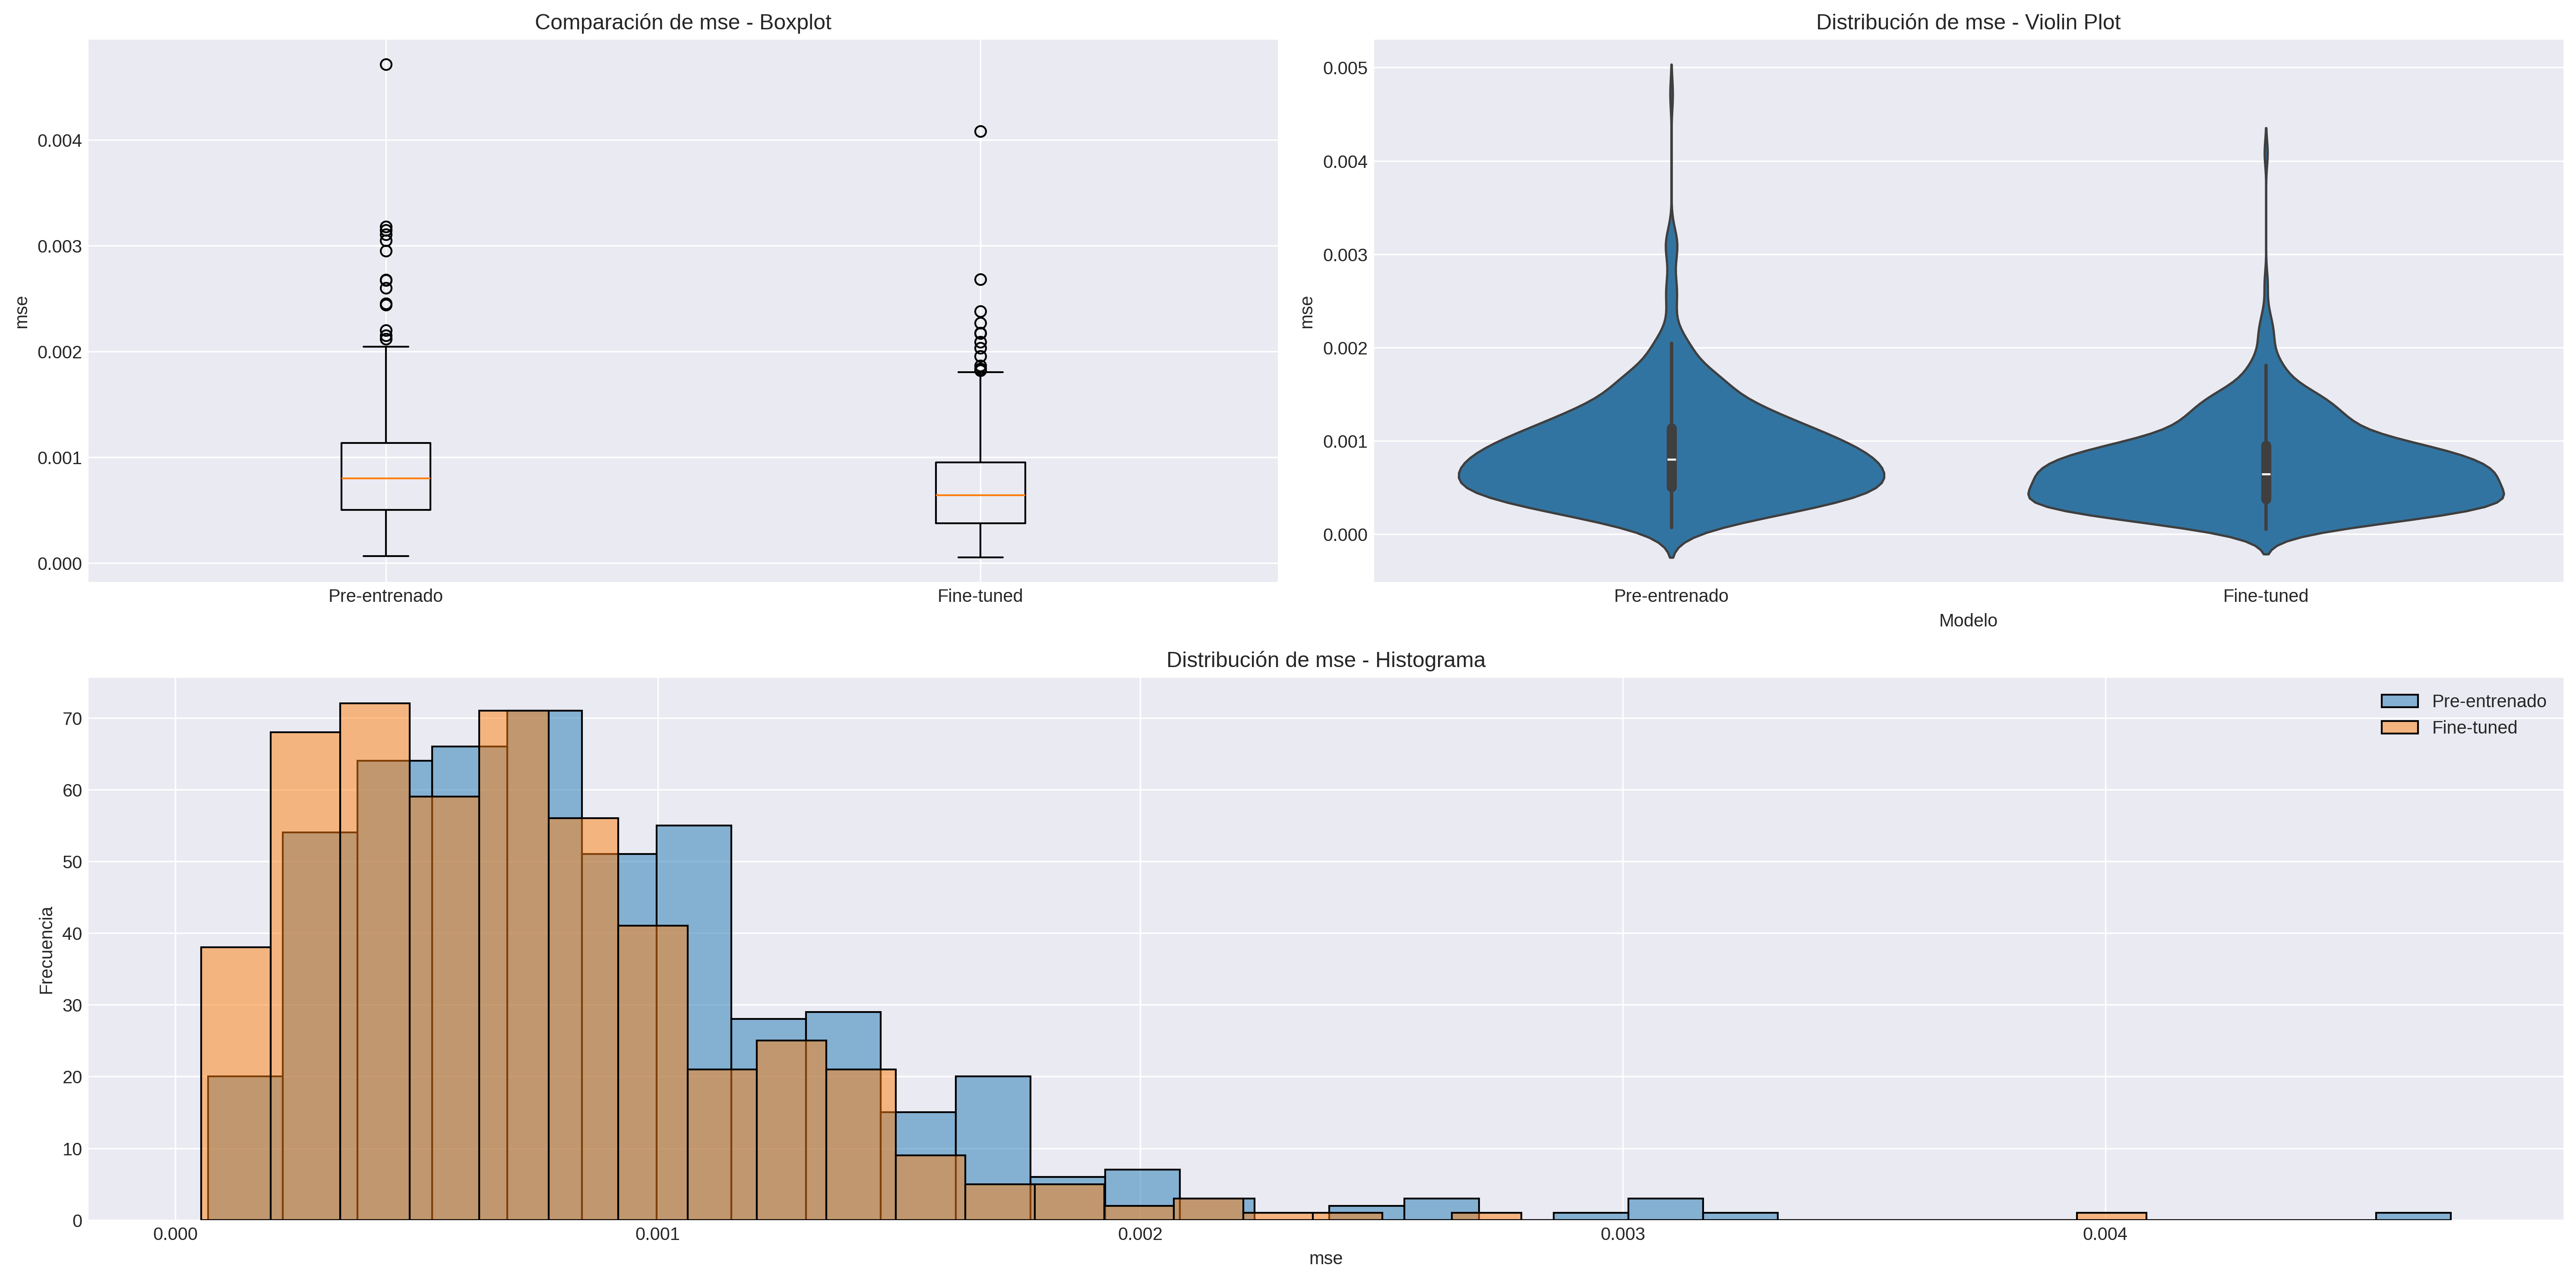
\includegraphics[width=\textwidth]{Images/comparison_plots_mse_sup.png}
            \caption{Comparación entre fine-tuning (FT) completo y modelo pre-entrenado}
            \label{fig:mse_no_phy}
        \end{subfigure}
        
        \caption{Análisis comparativo del Error Cuadrático Medio (MSE) entre el modelo pre-entrenado y las variantes de fine-tuning implementadas. a) Comparación entre fine-tuning sin componente física y modelo pre-entrenado. b) Comparación entre fine-tuning sin componente estructural y modelo pre-entrenado. c) Comparación entre fine-tuning completo y modelo pre-entrenado.}
        \label{fig:mse_analysis}
    \end{figure}
\end{figure}


\paragraph{Fine-tuning Completo (FT)}
El modelo con fine-tuning completo demuestra una mejora sustancial en términos del MSE. El error medio se redujo de $8.91 \times 10^{-4}$ en el modelo pre-entrenado a $7.26 \times 10^{-4}$ en el modelo fine-tuned, representando una mejora del 18.46\%. Esta reducción es particularmente significativa porque el MSE penaliza más severamente los errores grandes, indicando que el fine-tuning no solo mejora el rendimiento promedio sino que también reduce la incidencia de errores de gran magnitud.

La reducción en la variabilidad de los errores se evidencia en la disminución de la desviación estándar de $5.51 \times 10^{-4}$ a $4.64 \times 10^{-4}$. El rango de errores también se contrajo favorablemente, con el valor mínimo mejorando ligeramente de $6.8 \times 10^{-5}$ a $5.4 \times 10^{-5}$ y el máximo reduciéndose de $4.716 \times 10^{-3}$ a $4.086 \times 10^{-3}$. 

El análisis estadístico confirma la significancia de estas mejoras. A pesar de que las pruebas de Shapiro-Wilk ($W = 0.8855$ y $W = 0.8997$, ambas con $p < 0.001$) indican que las distribuciones no siguen una distribución normal, tanto la prueba $t$ pareada ($t = 12.3630$, $p < 0.001$) como la prueba no paramétrica de Wilcoxon ($W = 25146.0000$, $p < 0.001)$ confirman que la diferencia es estadísticamente significativa. El tamaño del efecto ($d$ de $Cohen = 0.3231$) indica una mejora de magnitud media.

\paragraph{Fine-tuning sin Componente Física (FT No-Physical)}
La eliminación de la componente física en el entrenamiento resulta en un deterioro notable del rendimiento. El MSE medio aumentó a $1.004 \times 10^{-3}$, lo que representa un empeoramiento del 12.69\% respecto al modelo pre-entrenado. Este incremento en el error viene acompañado de un aumento en la variabilidad, con una desviación estándar de $5.90 \times 10^{-4}$ y una expansión del rango de errores (mínimo: $1.00 \times 10^{-4}$, máximo: $5.131 \times 10^{-3}$).

Las pruebas estadísticas confirman que este deterioro es significativo, con un estadístico $t$ de $-11.9974$ $(p < 0.001)$ y un estadístico de Wilcoxon $W = 26066.0000$ ($p < 0.001$). El tamaño del efecto ($d$ de $Cohen = -0.1981$) indica que, aunque el impacto es negativo, su magnitud es relativamente pequeña en comparación con otros ablaciones.

\paragraph{Fine-tuning sin Componente Estructural (FT No-Structural)}
La ausencia de la componente estructural produce el deterioro más significativo en términos del MSE. El error medio aumentó a $1.119 \times 10^{-3}$, representando un empeoramiento del 25.69\% respecto al modelo pre-entrenado. Este incremento sustancial en el MSE es particularmente preocupante dado que indica un aumento en la frecuencia y magnitud de los errores grandes de reconstrucción.

La distribución de errores muestra un desplazamiento sistemático hacia valores más altos, con un valor mínimo de $1.95 \times 10^{-4}$ y un máximo de $4.834 \times 10^{-3}$. El análisis estadístico confirma la gravedad de este deterioro, con un estadístico $t$ de $-21.1018$ $(p < 0.001)$ y un estadístico de Wilcoxon $W = 10718.0000$ $(p < 0.001)$. El tamaño del efecto ($d$ de $Cohen = -0.4220$) indica un impacto negativo de magnitud media, subrayando la importancia crítica de la componente estructural en la función de pérdida.

Este análisis del MSE refuerza las conclusiones obtenidas del MAE, demostrando que la eliminación de cualquier componente de la función de pérdida resulta en un deterioro significativo del rendimiento, siendo la componente estructural particularmente crucial para mantener la calidad de la reconstrucción.

\subsubsection{Error Relativo Medio Normalizado (NRMSE)}


El Error Cuadrático Medio Normalizado (NRMSE) proporciona una medida del error que es independiente de la escala de los datos, facilitando la comparación entre diferentes conjuntos de datos o variables. Al normalizar el error, esta métrica nos permite evaluar la calidad relativa de la reconstrucción en términos porcentuales respecto a la magnitud de los datos originales.


\begin{figure}[H]
    \centering
    \begin{subfigure}[b]{0.48\textwidth}
        \centering
        % FT No-Physical vs Baseline
        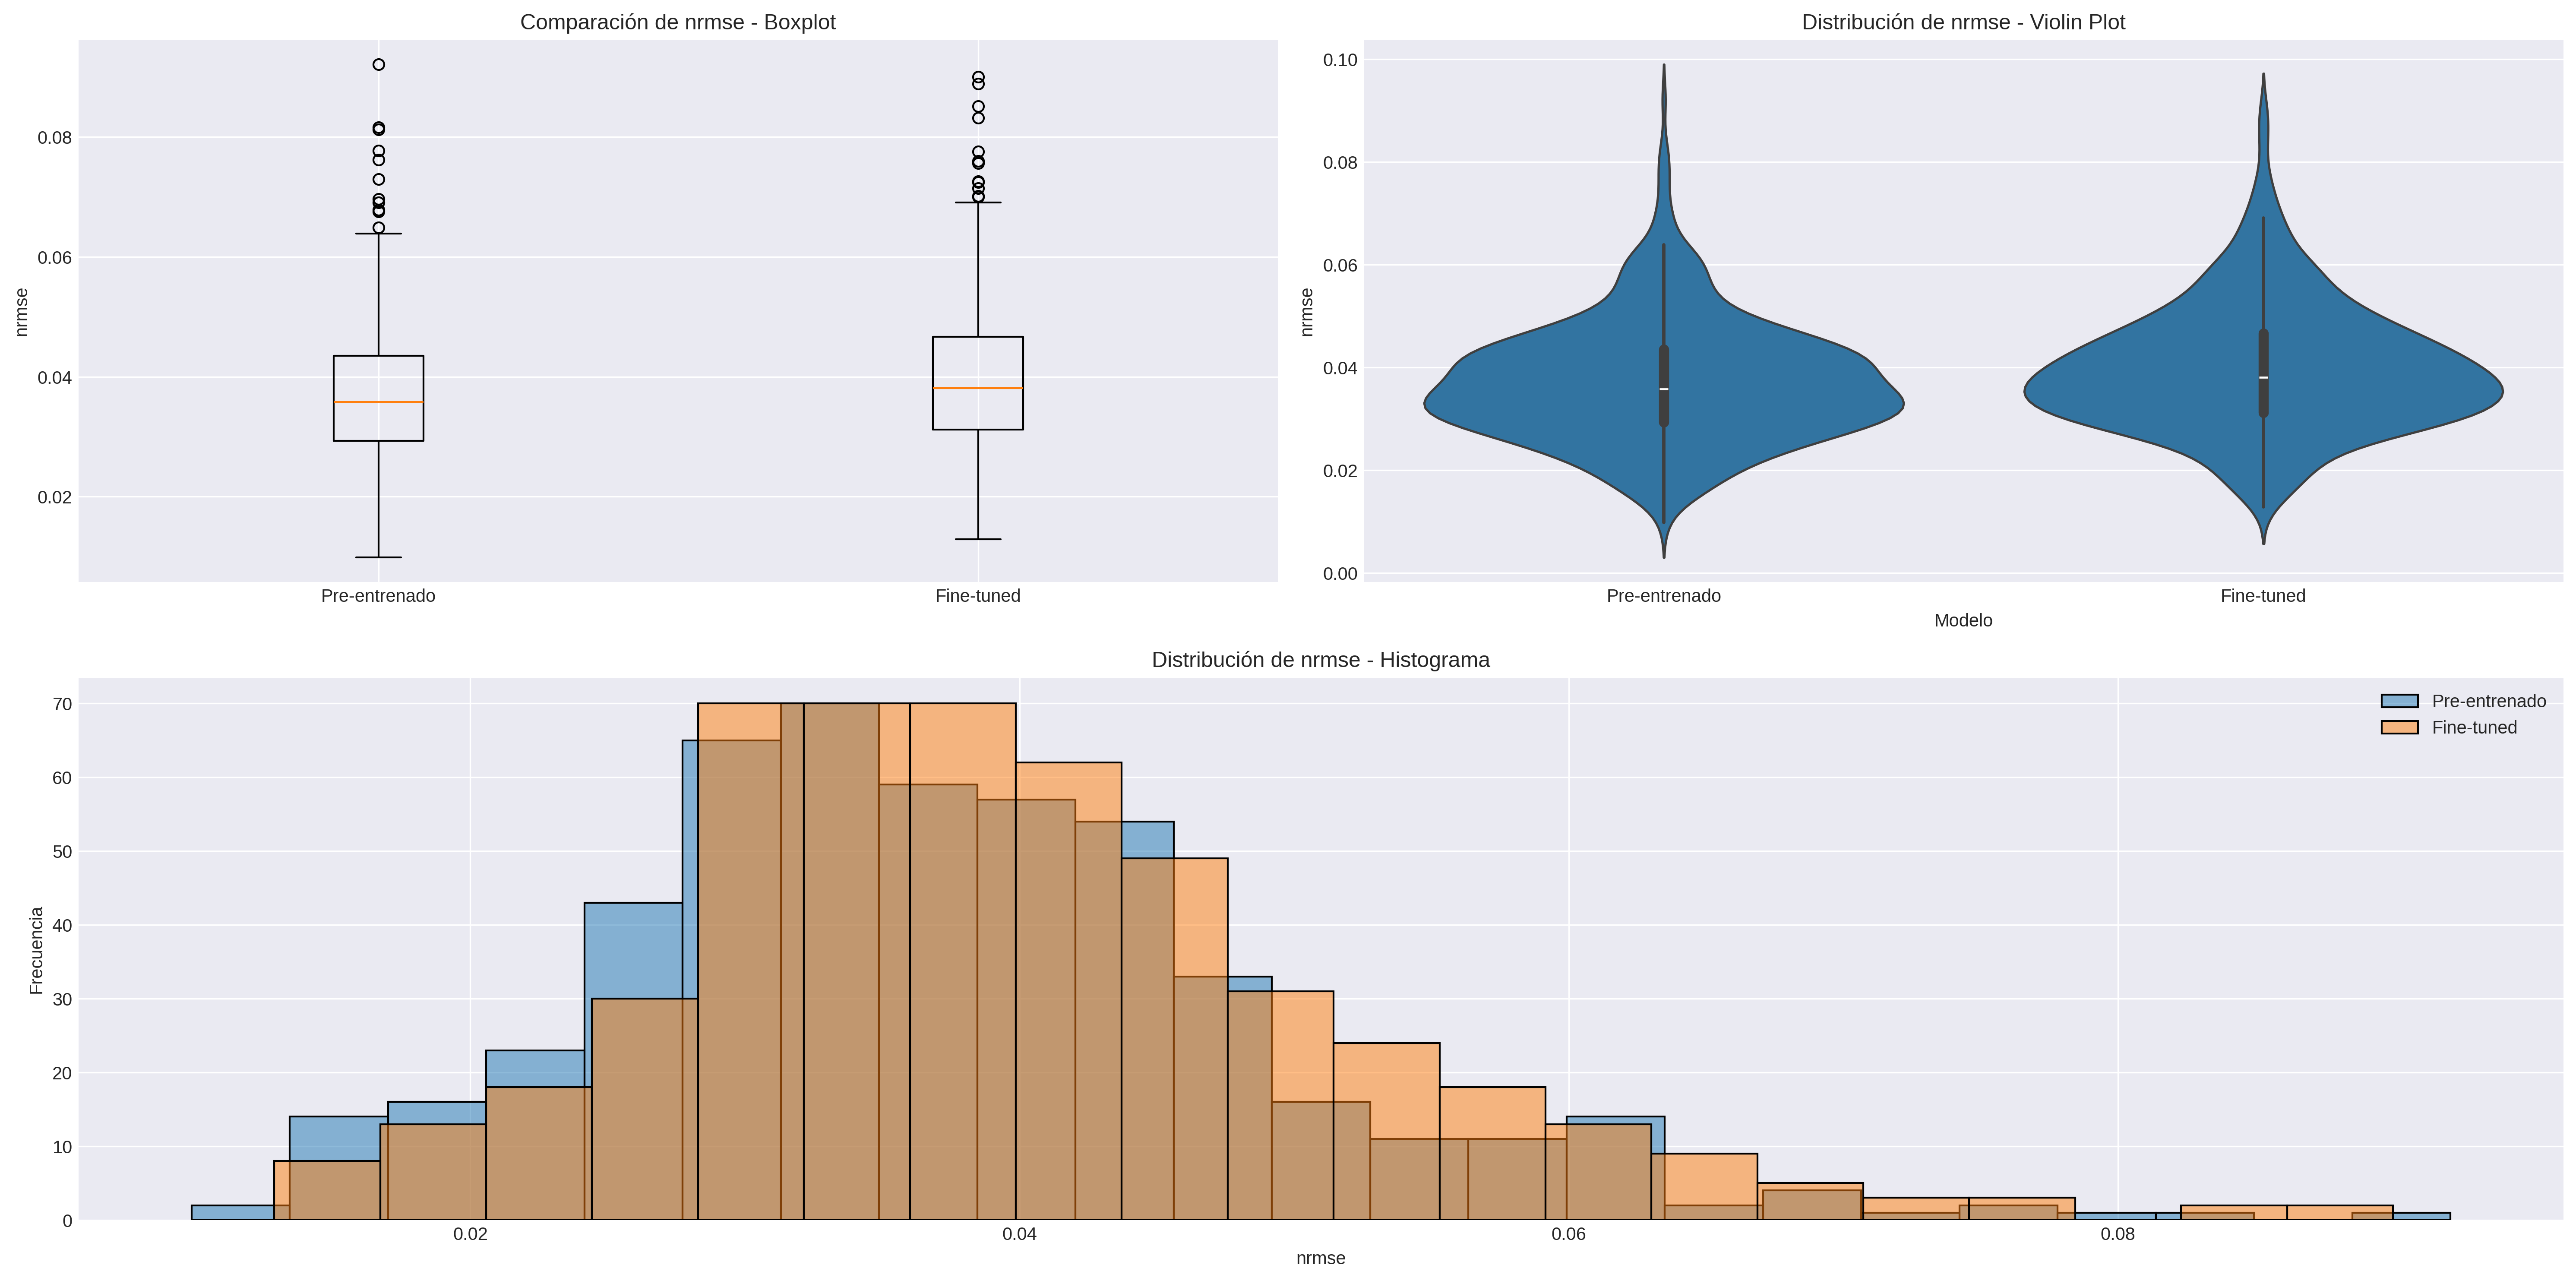
\includegraphics[width=\textwidth]{Images/comparison_plots_nrmse_no_phy.png}
        \caption{Comparación entre fine-tuning sin componente física y modelo pre-entrenado}
        \label{fig:nrmse_hist}
    \end{subfigure}
    \hfill
    \begin{subfigure}[b]{0.48\textwidth}
        \centering
        % FT No-Structural vs Baseline
        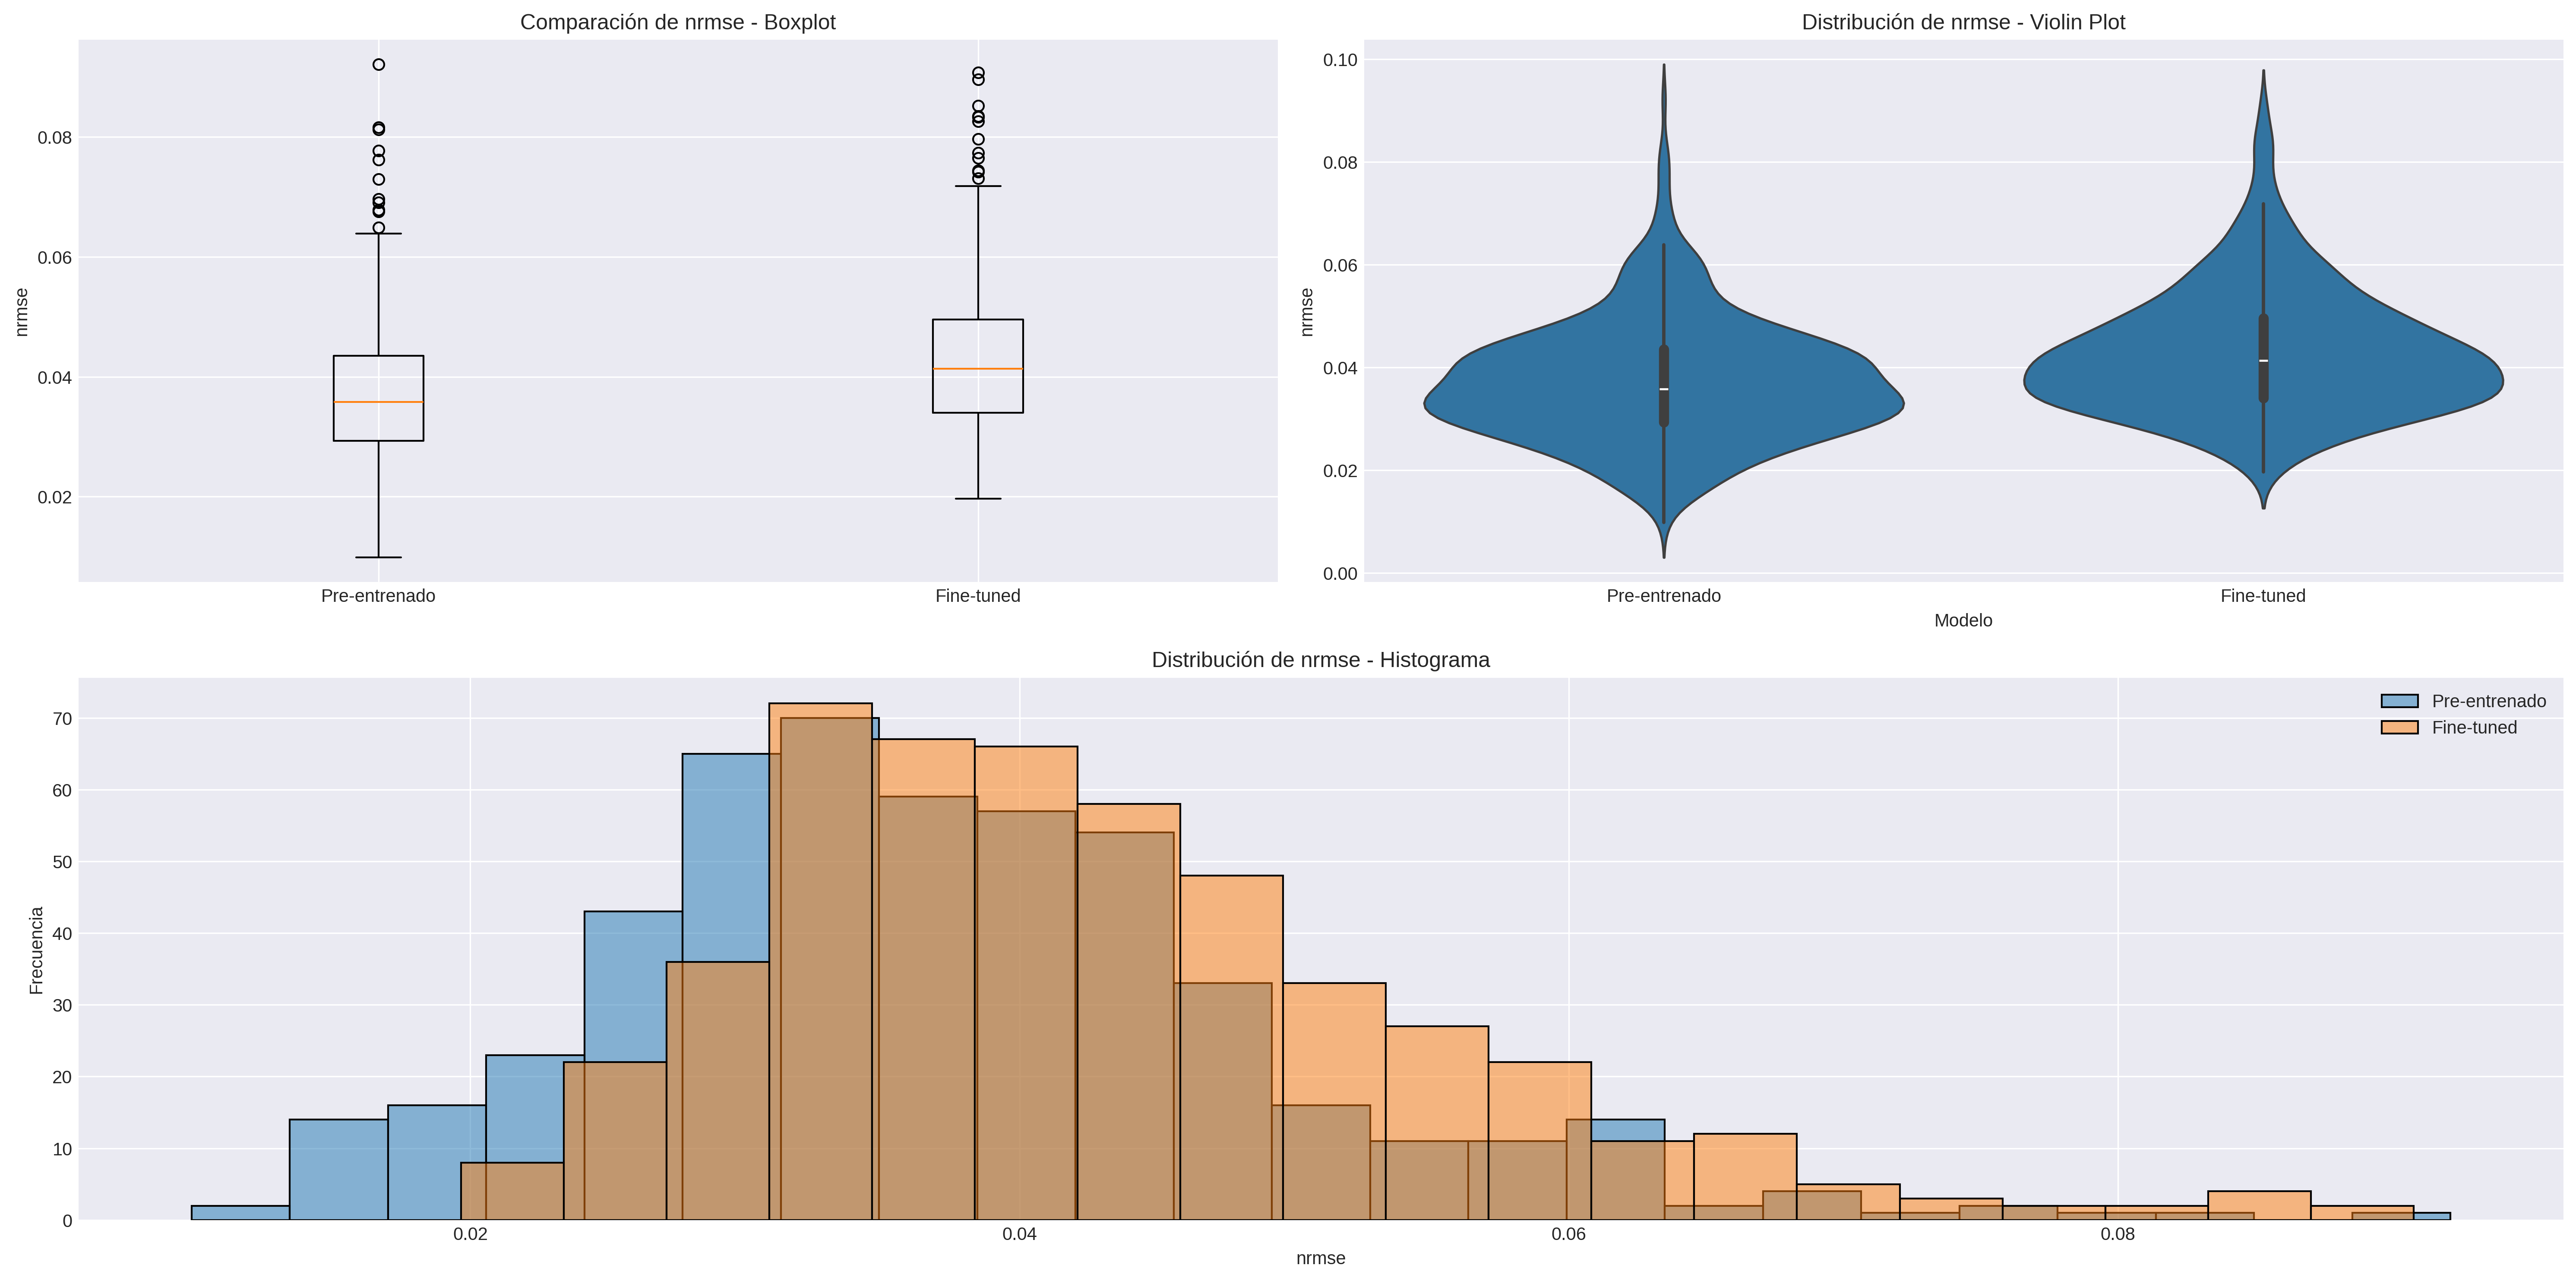
\includegraphics[width=\textwidth]{Images/comparison_plots_nrmse_no_struct.png}
        \caption{Comparación entre fine-tuning sin componente estructural y modelo pre-entrenado}
        \label{fig:nrmse_violin}
    \end{subfigure}
    
    \vspace{0.5cm}
    
    \begin{subfigure}[b]{0.7\textwidth}
        \centering
        % FT vs Baseline
        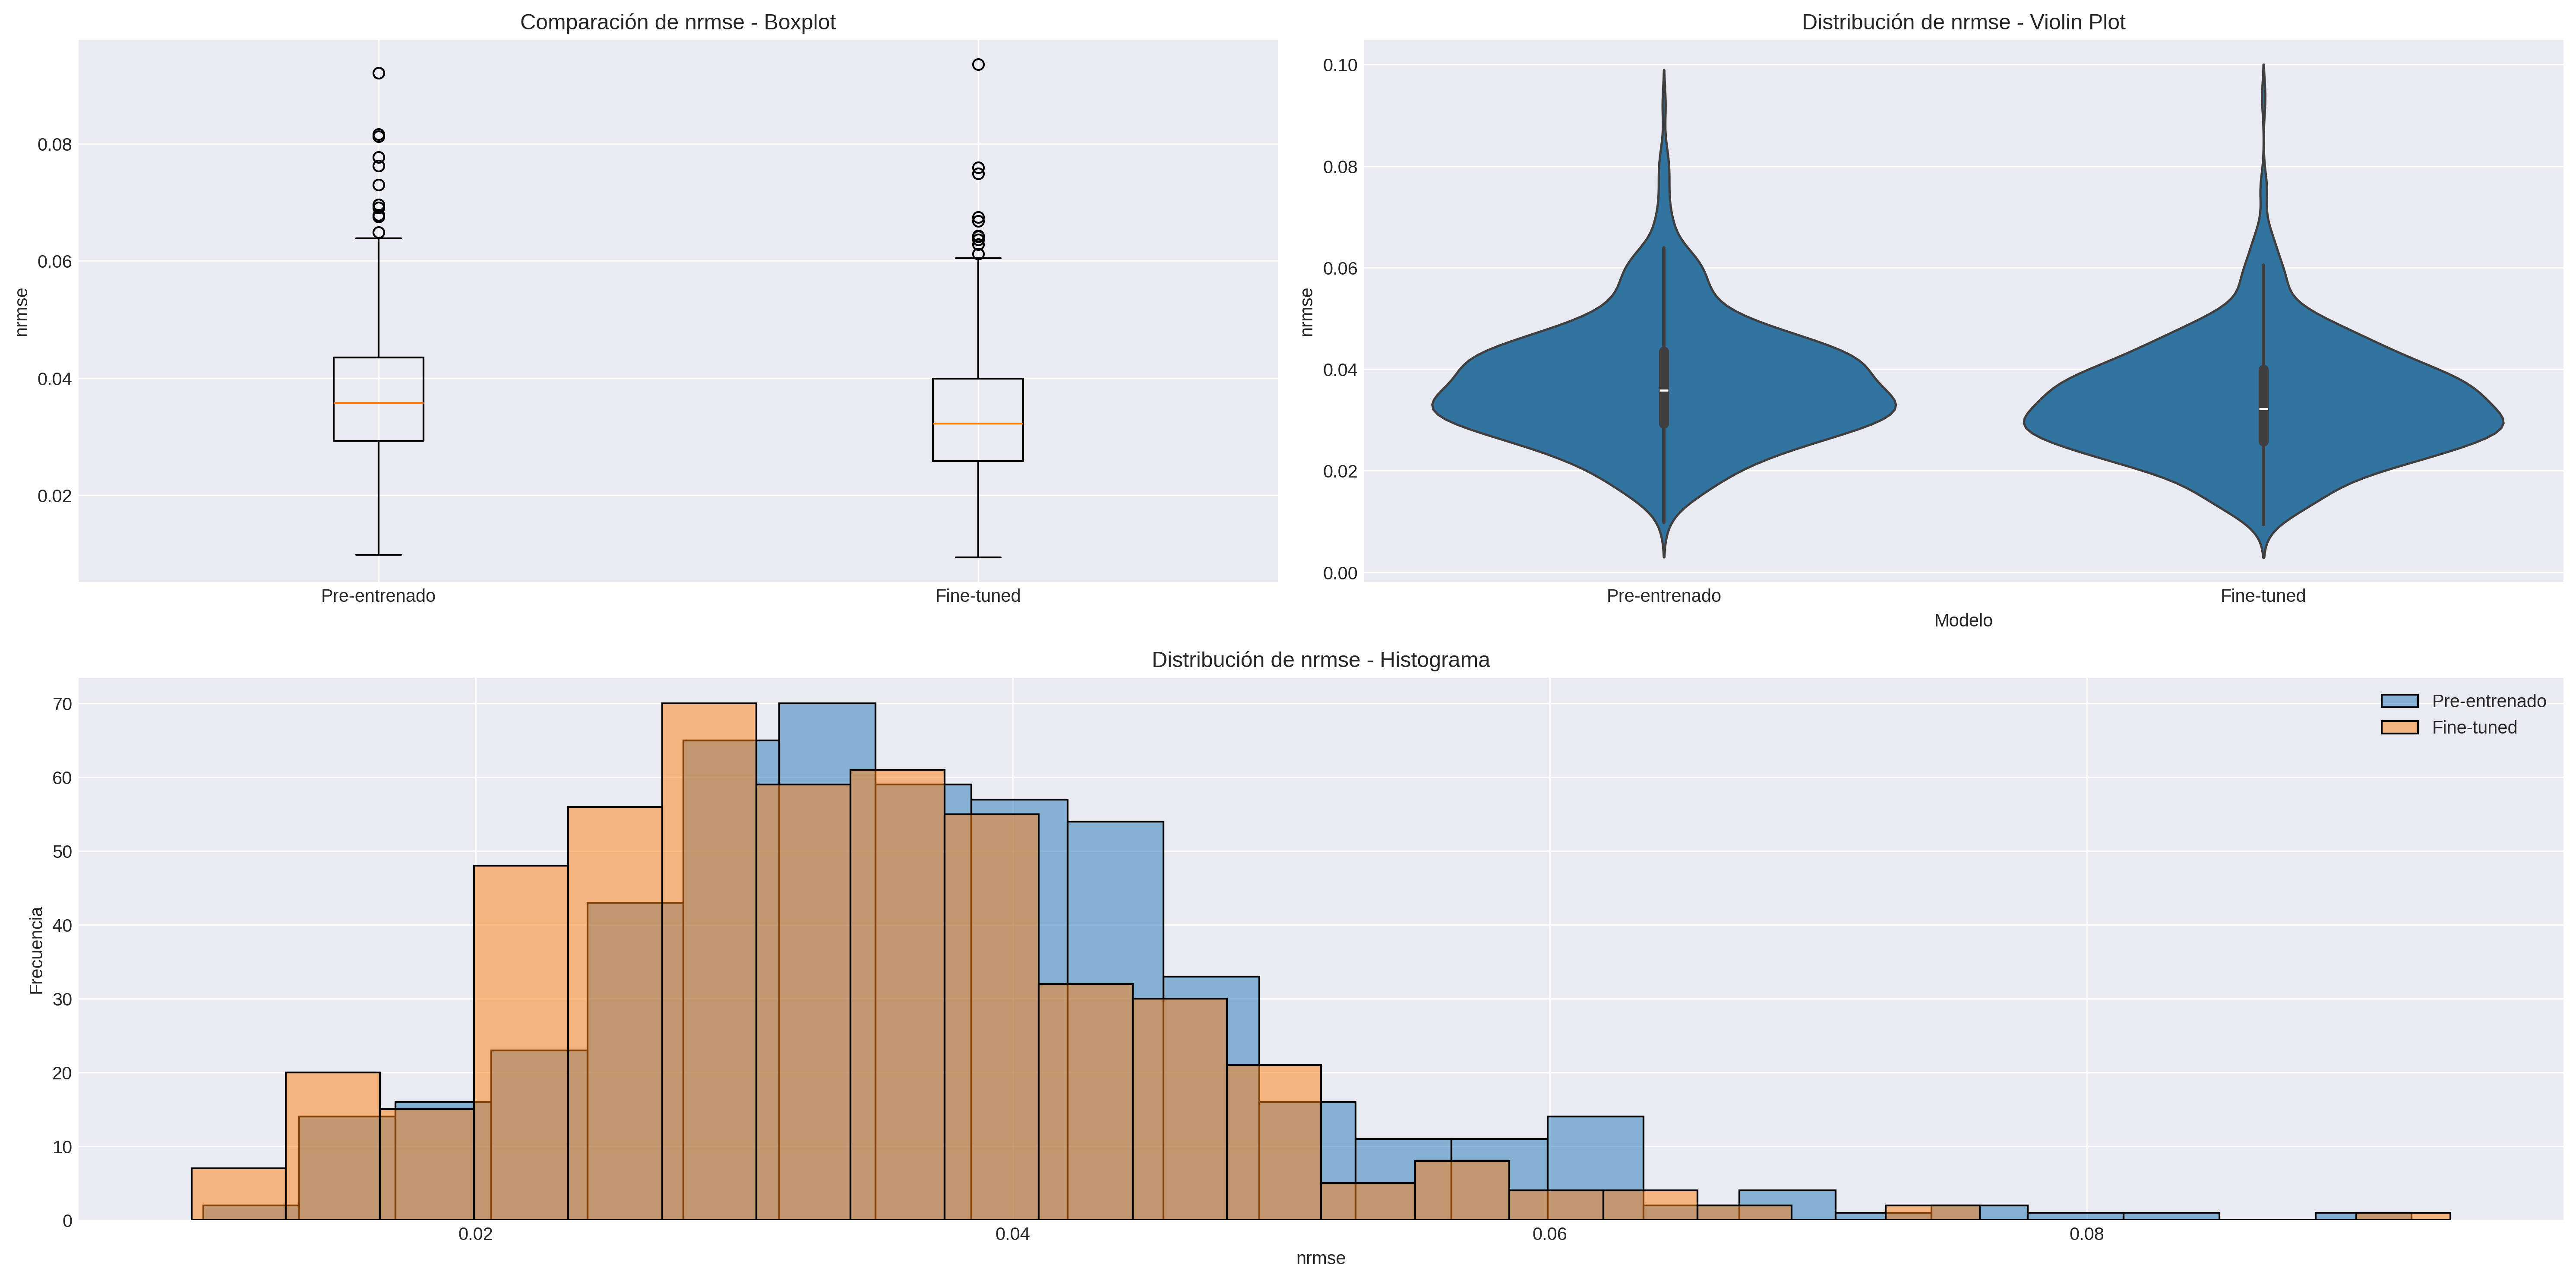
\includegraphics[width=\textwidth]{Images/comparison_plots_nrmse_sup.png}
        \caption{Comparación entre fine-tuning (FT) completo y modelo pre-entrenado}
        \label{fig:nrmse_box}
    \end{subfigure}
    
    \caption{Análisis comparativo del Error Relativo Medio Normalizado (NRMSE) entre el modelo pre-entrenado y las variantes de fine-tuning implementadas. a) Comparación entre fine-tuning sin componente física y modelo pre-entrenado. b) Comparación entre fine-tuning sin componente estructural y modelo pre-entrenado. c) Comparación entre fine-tuning completo y modelo pre-entrenado.}
    \label{fig:nrmse_analysis}
\end{figure}



\paragraph{Fine-tuning Completo (FT)}
El modelo con fine-tuning completo demuestra una mejora significativa en la precisión de reconstrucción normalizada. El NRMSE medio se redujo de 0.037209 (3.72\%) en el modelo pre-entrenado a 0.033431 (3.34\%) en el modelo fine-tuned, representando una mejora del 10.15\%. Esta reducción es particularmente relevante porque indica que el modelo mejoró su capacidad de reconstrucción de manera consistente a través de diferentes escalas de magnitud en los datos.

La consistencia de la mejora se refleja en la reducción de la variabilidad, con una disminución en la desviación estándar de 0.011857 a 0.011228. El rango de errores también muestra una mejora, con el valor mínimo reduciéndose de 0.009851 (0.99\%) a 0.009414 (0.94\%). El análisis estadístico confirma la significancia de estas mejoras a través de múltiples pruebas:

\begin{itemize}
    \item La prueba t pareada ($t = 13.3137$, $p < 0.001$) y la prueba de Wilcoxon ($W = 24360.0000$, $p < 0.001$) confirman que la diferencia es estadísticamente significativa
    \item El tamaño del efecto ($d$ de $Cohen = 0.3272$) indica una mejora de magnitud media
    \item Las pruebas de Shapiro-Wilk ($W \approx 0.966$ para ambas distribuciones, $p < 0.001$) sugieren que el análisis no paramétrico es particularmente relevante
\end{itemize}

\paragraph{Fine-tuning sin Componente Física (FT No-Physical)}
La eliminación de la componente física resulta en un deterioro notable del rendimiento normalizado. El NRMSE medio aumentó a 0.039862 (3.99\%), representando un empeoramiento del 7.13\% respecto al modelo pre-entrenado. Este incremento en el error normalizado sugiere que la ausencia de la componente física afecta la capacidad del modelo para capturar las relaciones subyacentes en los datos, independientemente de su escala.

La distribución de errores muestra un desplazamiento sistemático hacia valores más altos, con:

\begin{itemize}
    \item Un incremento en el valor mínimo a 0.012861 (1.29\%)
    \item Un aumento en la variabilidad (desviación estándar de 0.012413)
    \item Una modificación en la forma de la distribución, como lo indica la prueba de Shapiro-Wilk ($W = 0.9647$, $p < 0.001$)
\end{itemize}

El análisis estadístico confirma que este deterioro es significativo ($t = -12.3593$, $p < 0.001$; $W = 25214.0000$, $p < 0.001$), aunque el tamaño del efecto ($d$ de $Cohen = -0.2186$) sugiere que el impacto, aunque negativo, es relativamente moderado.

\paragraph{Fine-tuning sin Componente Estructural (FT No-Structural)}
La ausencia de la componente estructural produce el deterioro más significativo en términos del NRMSE. El error medio aumentó a 0.042954 (4.30\%), lo que representa un empeoramiento del 15.44\% respecto al modelo pre-entrenado. Este incremento sustancial en el NRMSE es particularmente revelador porque indica que la componente estructural es fundamental para mantener la precisión de reconstrucción a través de diferentes escalas de magnitud.

El impacto negativo se manifiesta en múltiples aspectos:

\begin{itemize}
    \item Un aumento significativo en el valor mínimo del error a 0.019659 (1.97\%)
    \item Un incremento en la variabilidad (desviación estándar de 0.012241)
    \item Una alteración más pronunciada en la forma de la distribución ($W = 0.9475$, $p < 0.001$)
\end{itemize}

La significancia estadística de este deterioro se confirma mediante múltiples pruebas:

\begin{itemize}
    \item La prueba t pareada muestra un efecto fuerte ($t = -20.0658$, $p < 0.001$)
    \item La prueba de Wilcoxon corrobora estos resultados ($W = 9258.0000$, $p < 0.001$)
    \item El tamaño del efecto ($d$ de $Cohen = -0.4767$) indica un impacto negativo de magnitud media a grande
\end{itemize}

Este análisis del NRMSE complementa y refuerza las conclusiones obtenidas del MSE y MAE, proporcionando una perspectiva normalizada que demuestra cómo los componentes de la función de pérdida afectan la calidad de reconstrucción independientemente de la escala de los datos. La componente estructural se revela nuevamente como el elemento más crítico para mantener la precisión de la reconstrucción.




\subsubsection{Peak Signal-to-Noise Ratio (PSNR)}

El Peak Signal-to-Noise Ratio (PSNR) es una métrica logarítmica que evalúa la calidad de la reconstrucción en términos de la relación entre la máxima señal posible y el ruido introducido por el proceso de reconstrucción. A diferencia de las métricas anteriores, un valor más alto de PSNR indica una mejor calidad de reconstrucción, ya que representa una mejor relación señal-ruido.


\begin{figure}[H]
    \centering
    \begin{subfigure}[b]{0.48\textwidth}
        \centering
        % FT No-Physical vs Baseline
        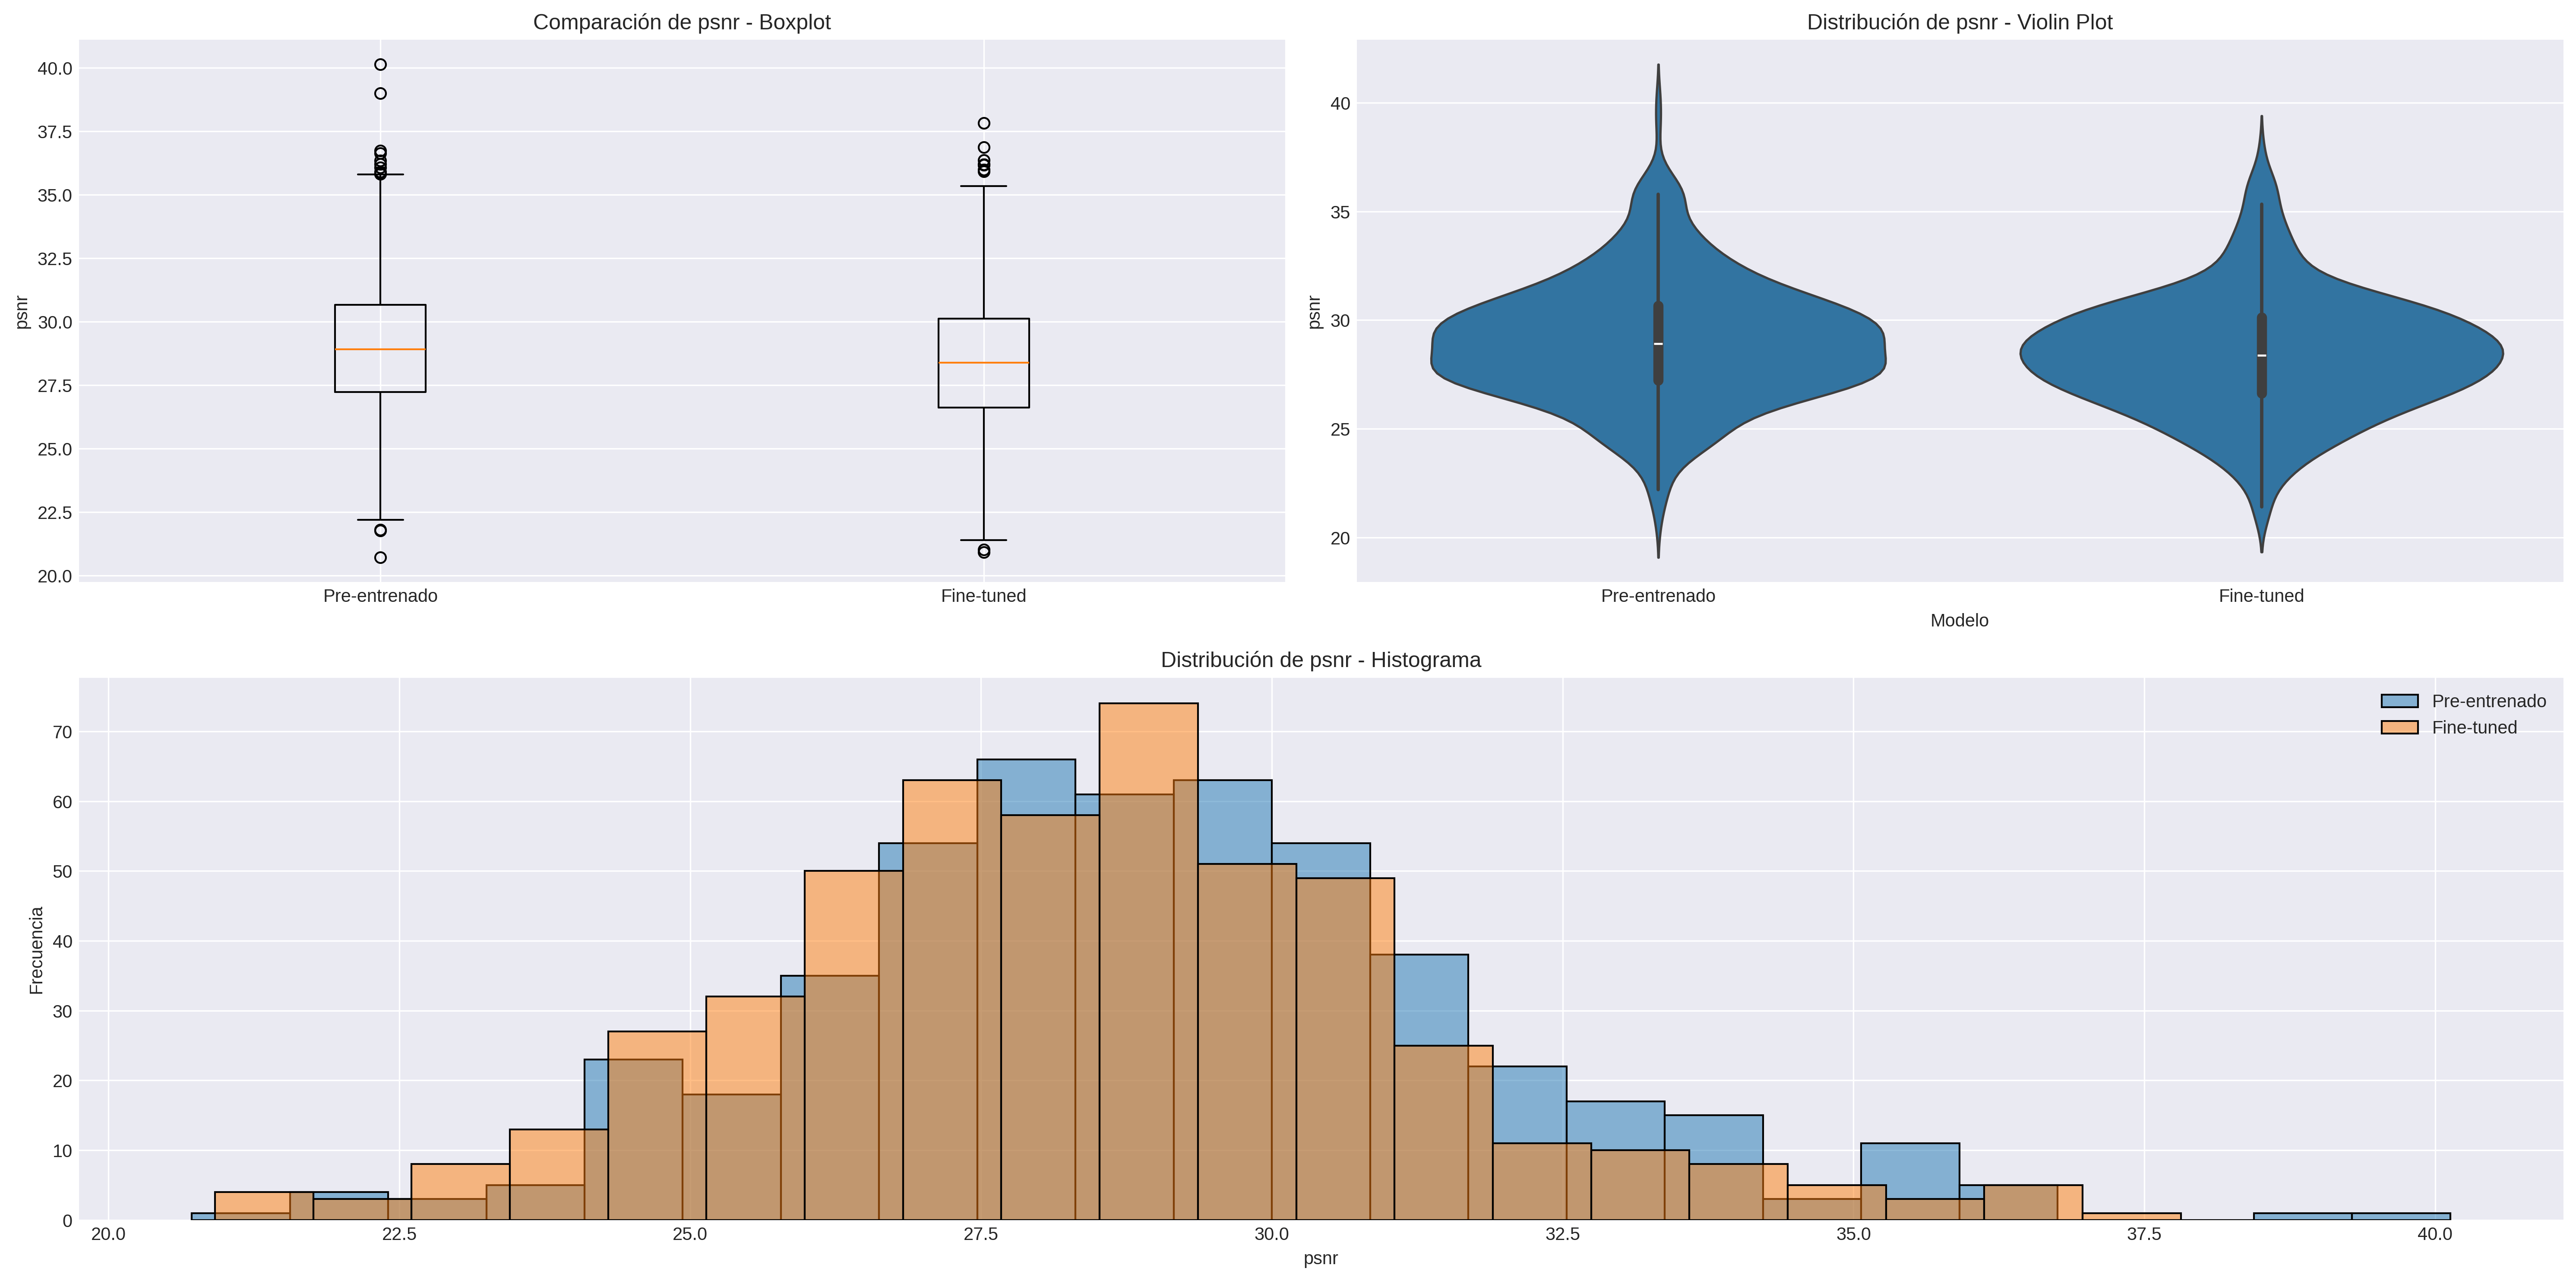
\includegraphics[width=\textwidth]{Images/comparison_plots_psnr_no_phy.png}
        \caption{Comparación entre fine-tuning sin componente física y modelo pre-entrenado}
        \label{fig:psnr_hist}
    \end{subfigure}
    \hfill
    \begin{subfigure}[b]{0.48\textwidth}
        \centering
        % FT No-Structural vs Baseline
        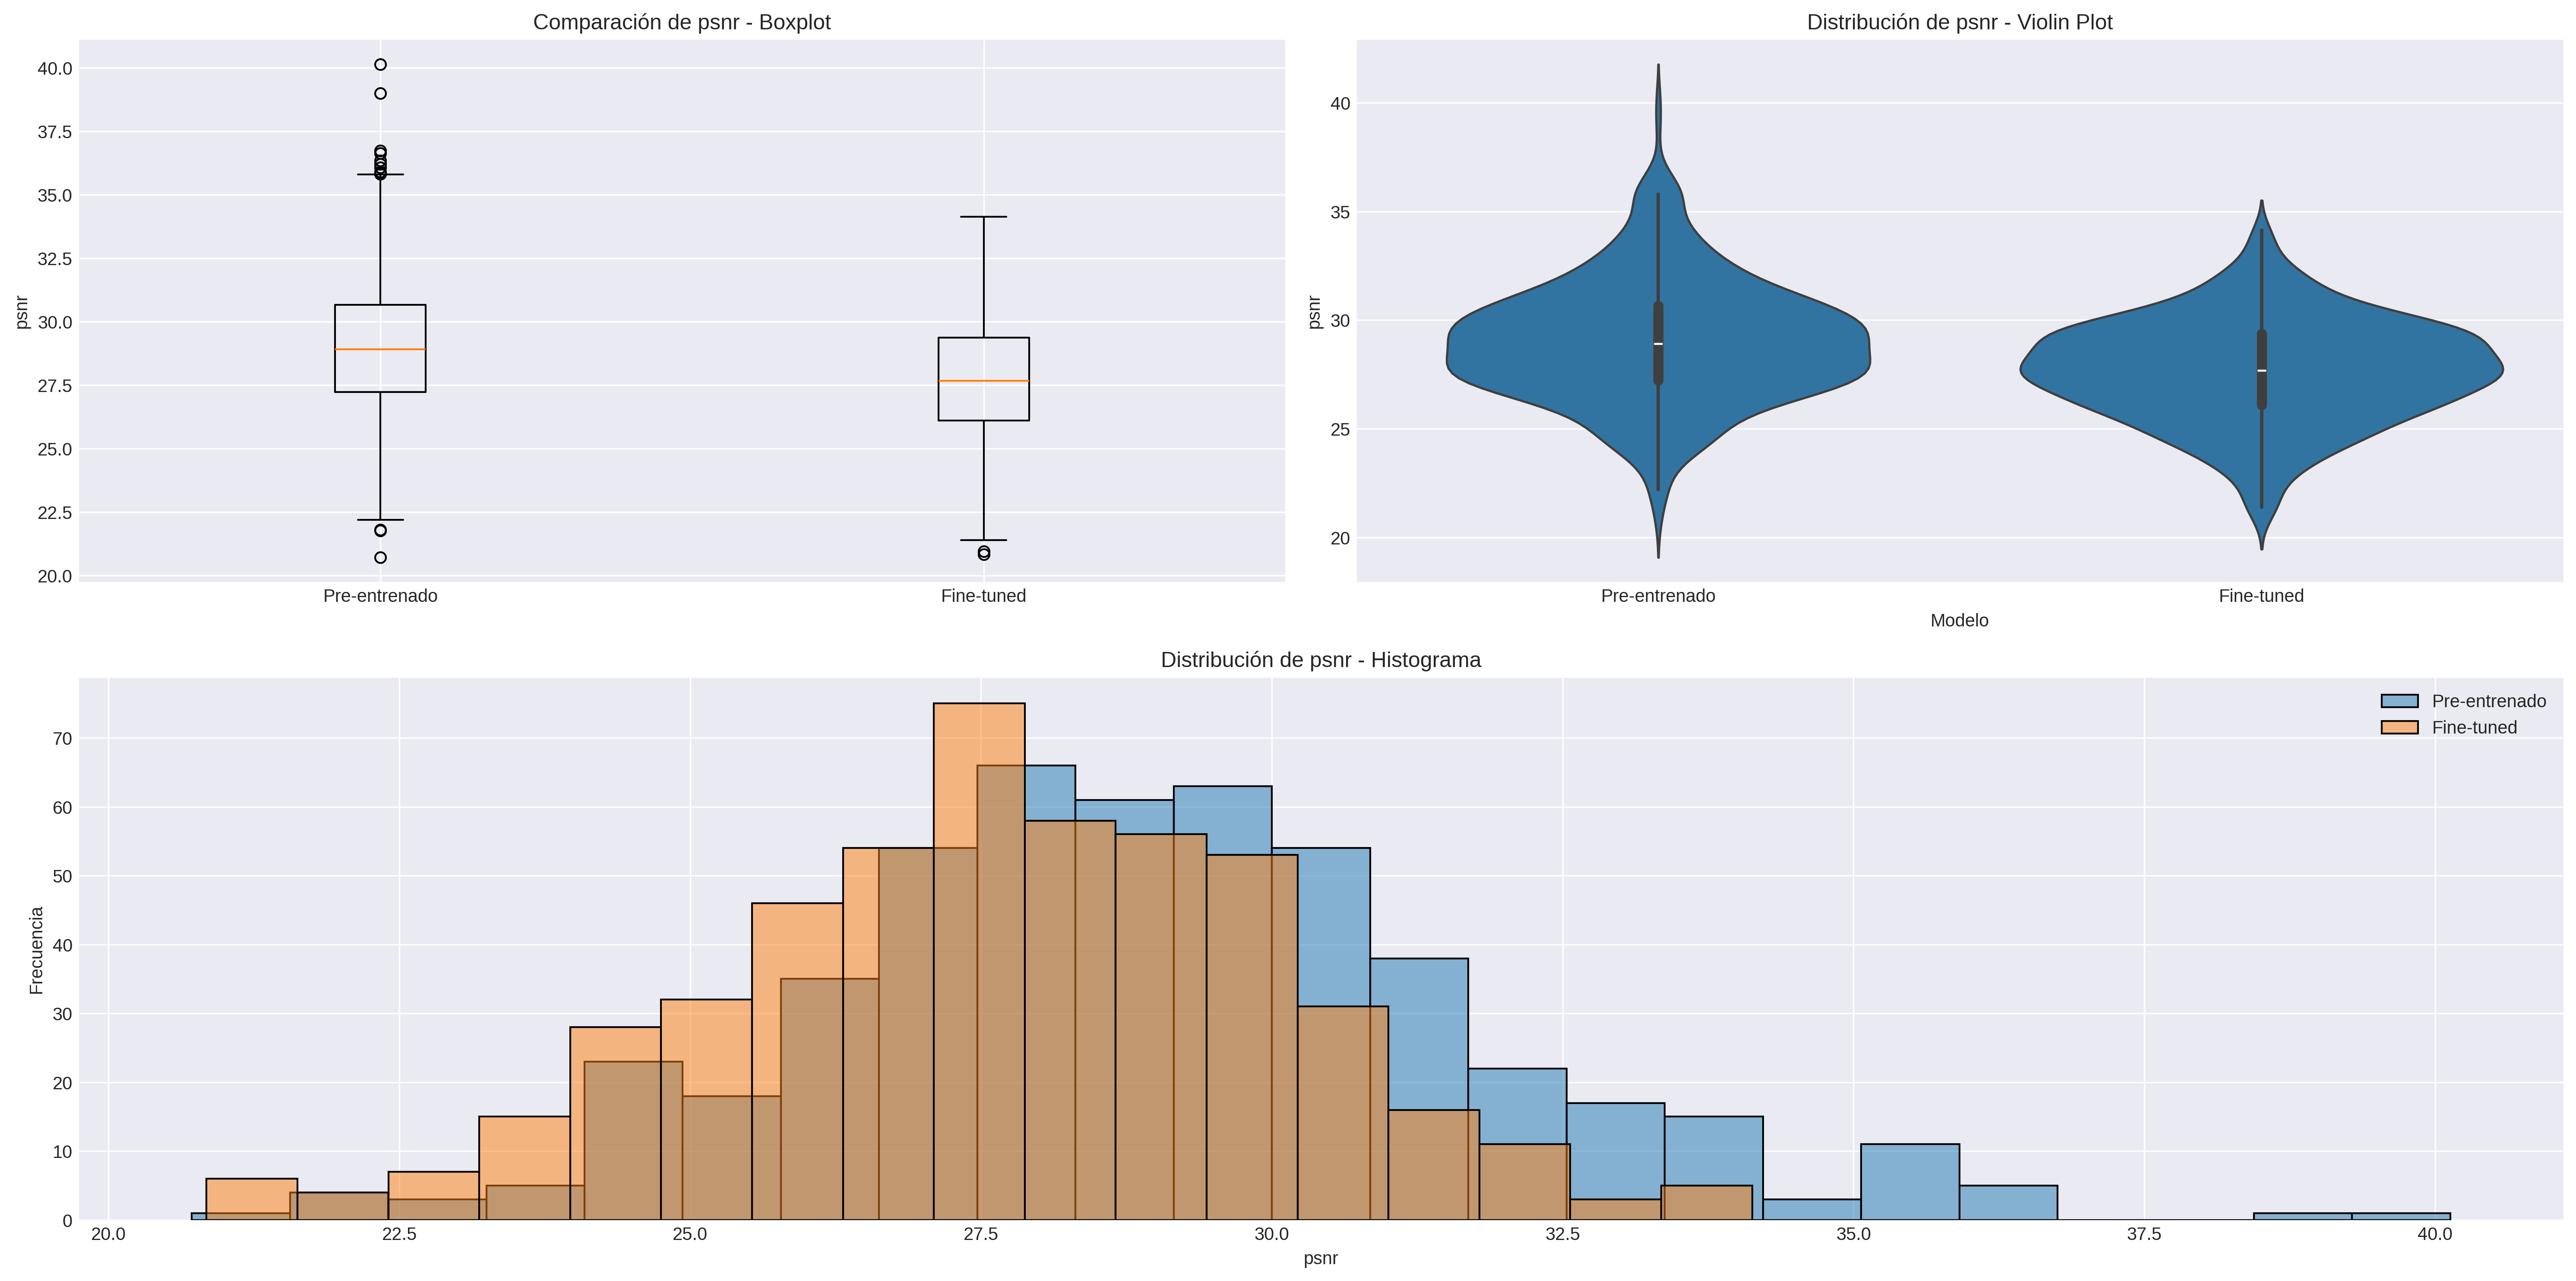
\includegraphics[width=\textwidth]{Images/comparison_plots_psnr_no_struct.png}
        \caption{Comparación entre fine-tuning sin componente estructural y modelo pre-entrenado}
        \label{fig:psnr_violin}
    \end{subfigure}
    
    \vspace{0.5cm}
    
    \begin{subfigure}[b]{0.7\textwidth}
        \centering
        % FT vs Baseline
        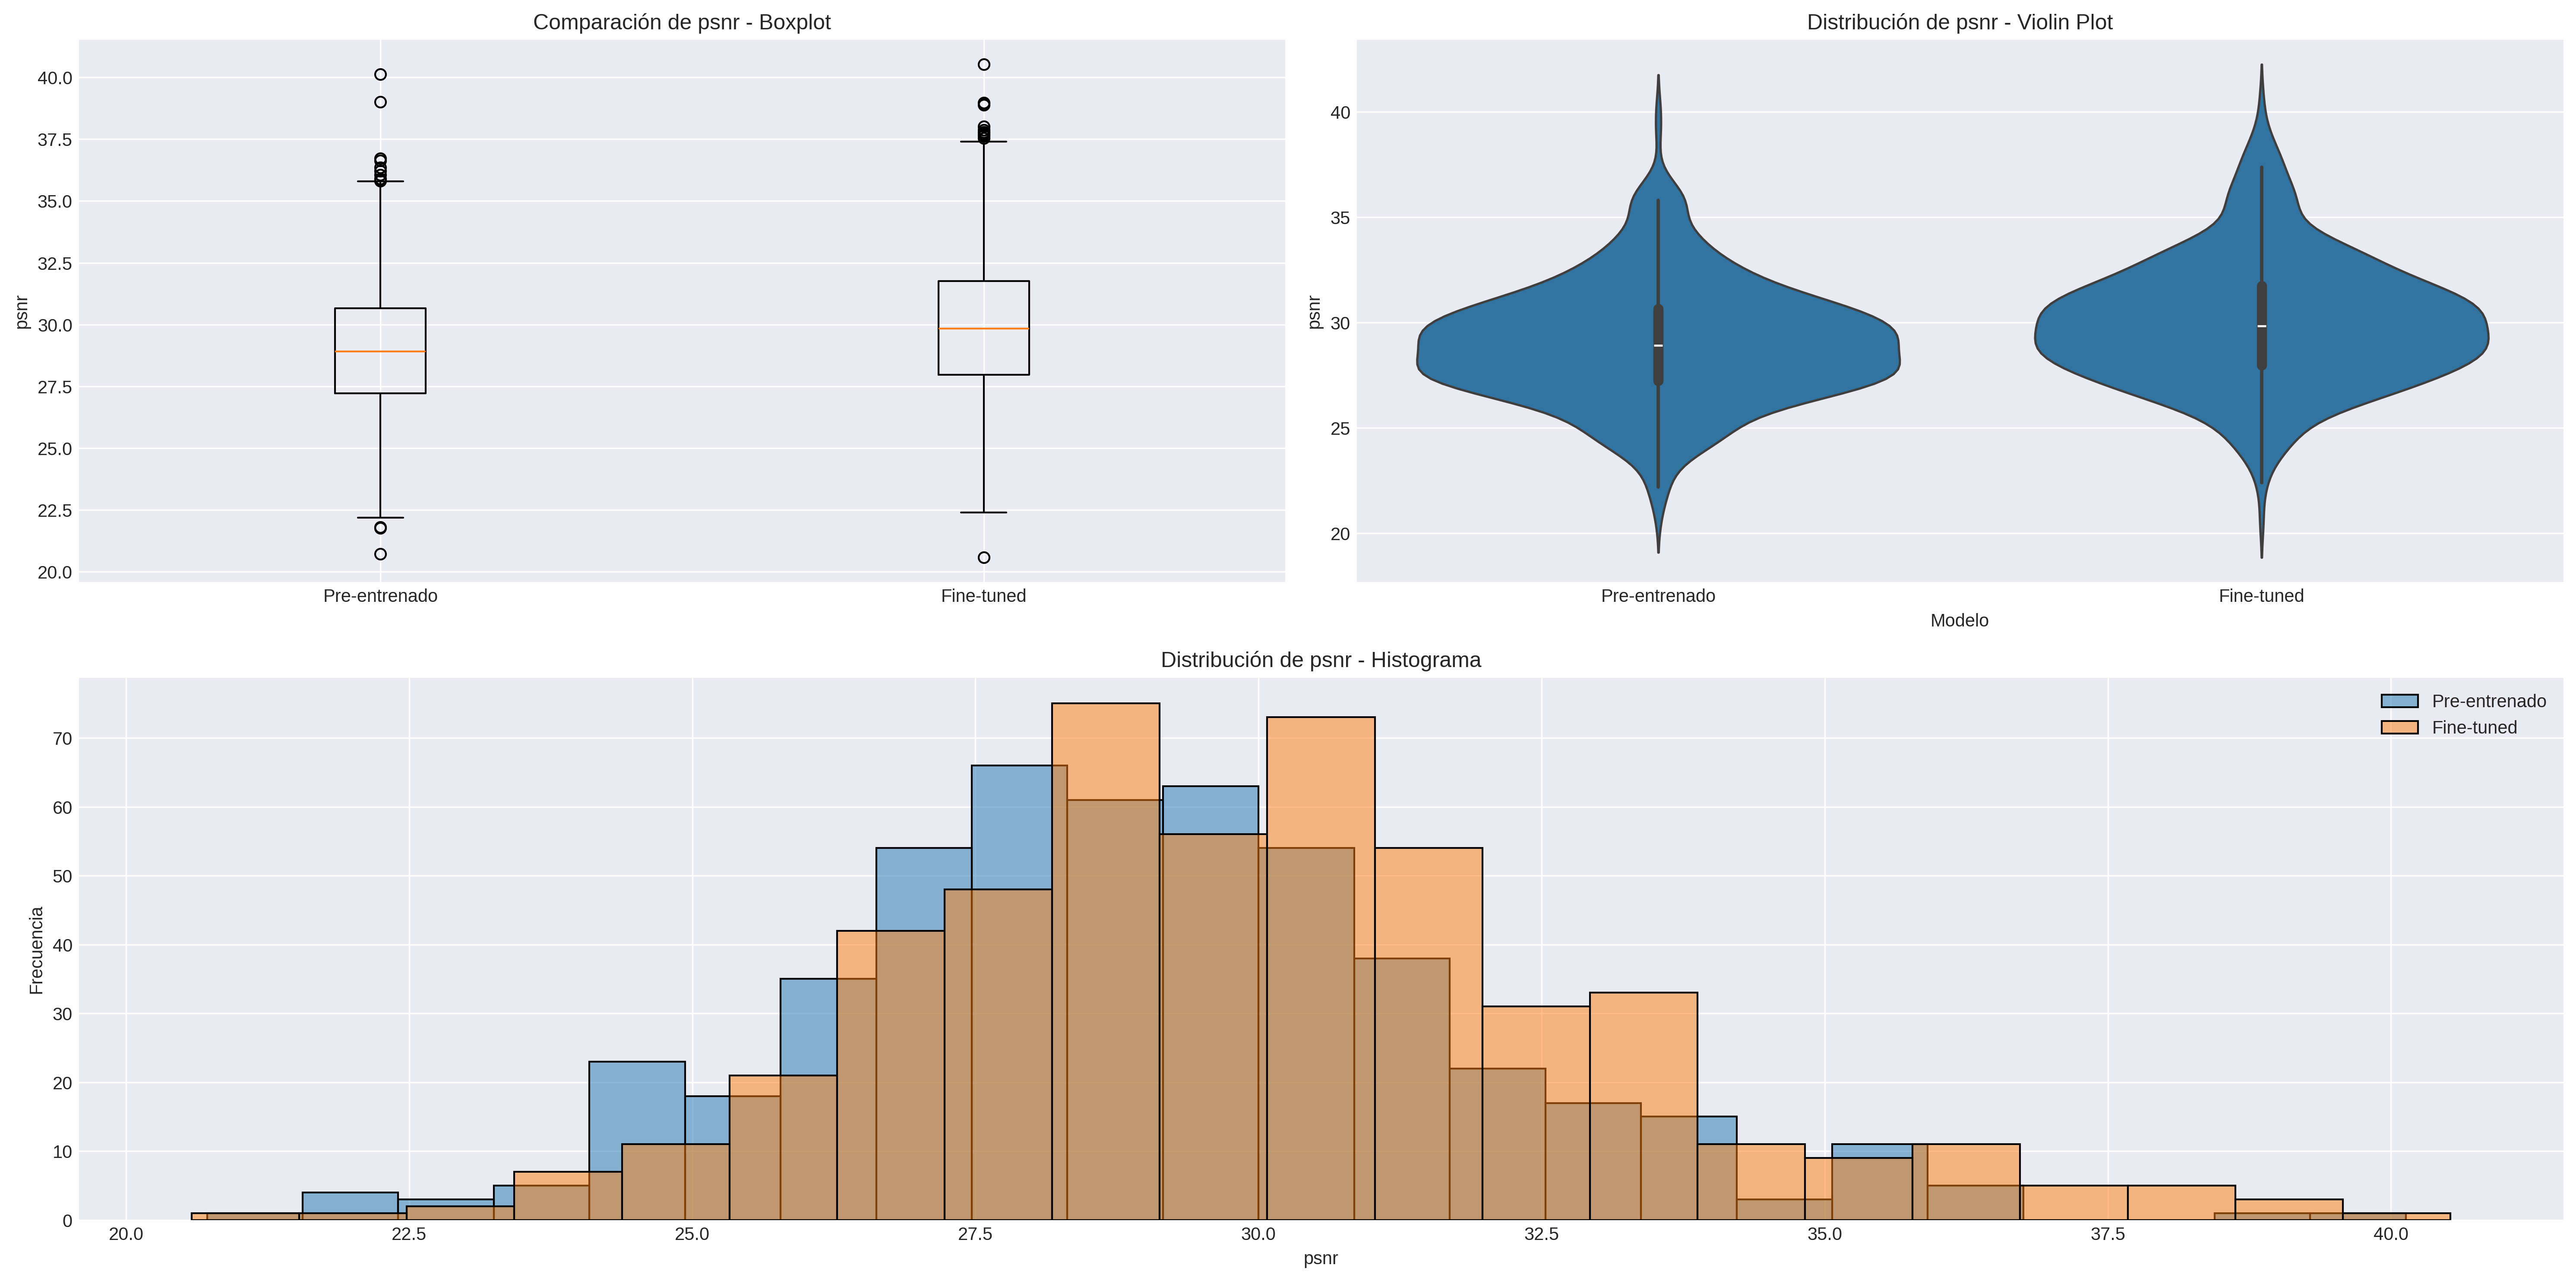
\includegraphics[width=\textwidth]{Images/comparison_plots_psnr_sup.png}
        \caption{Comparación entre fine-tuning (FT) completo y modelo pre-entrenado}
        \label{fig:psnr_box}
    \end{subfigure}
    
    \caption{Análisis comparativo del Peak Signal-to-Noise Ratio (PSNR) entre el modelo pre-entrenado y las variantes de fine-tuning implementadas. a) Comparación entre fine-tuning sin componente física y modelo pre-entrenado. b) Comparación entre fine-tuning sin componente estructural y modelo pre-entrenado. c) Comparación entre fine-tuning completo y modelo pre-entrenado.}
    \label{fig:psnr_analysis}
\end{figure}


\paragraph{Fine-tuning Completo (FT)}
El modelo con fine-tuning completo logra una mejora sustancial en la calidad de reconstrucción según el PSNR. El valor medio aumentó de 29.03 dB en el modelo pre-entrenado a 30.01 dB en el modelo fine-tuned, representando un incremento de aproximadamente 1 dB. Este aumento es significativo en el contexto del PSNR, donde incluso pequeñas mejoras en decibelios pueden representar diferencias notables en la calidad visual de la reconstrucción.

La distribución de los valores de PSNR muestra características interesantes:

\begin{itemize}
    \item Se observa un aumento en el rango dinámico, con el valor máximo mejorando de 40.13 dB a 40.52 dB
    \item La mediana aumentó de 28.92 dB a 29.84 dB, indicando una mejora consistente en la tendencia central
    \item La desviación estándar se incrementó ligeramente de 2.82 dB a 3.01 dB, sugiriendo una mayor variabilidad en la capacidad del modelo para manejar casos difíciles
\end{itemize}

El análisis estadístico confirma la significancia de estas mejoras:

\begin{itemize}
    \item La prueba $t$ pareada ($t = -13.0039$, $p < 0.001$) y la prueba de Wilcoxon ($W = 24581.0000$, $p < 0.001$) demuestran que el incremento en PSNR es estadísticamente significativo
    \item El tamaño del efecto ($d$ de $Cohen = -0.3375$) indica una mejora de magnitud media
    \item Las pruebas de Shapiro-Wilk sugieren ligeras desviaciones de la normalidad en ambas distribuciones
\end{itemize}

\paragraph{Fine-tuning sin Componente Física (FT No-Physical)}
La eliminación de la componente física resulta en una degradación notable de la calidad de reconstrucción. El PSNR medio disminuyó a 28.41 dB, representando una pérdida de aproximadamente 0.62 dB respecto al modelo pre-entrenado. Esta reducción es particularmente relevante porque indica un aumento en el ruido de reconstrucción cuando se omite la información física del proceso de entrenamiento.

Los cambios en la distribución del PSNR son reveladores:

\begin{itemize}
    \item El valor máximo se redujo significativamente a 37.81 dB
    \item La mediana descendió a 28.39 dB
    \item La desviación estándar se mantuvo similar (2.74 dB), sugiriendo que la degradación es consistente a través de diferentes casos
\end{itemize}

Las pruebas estadísticas confirman que este deterioro es significativo ($t = 11.8015$, $p < 0.001$; $W = 25972.0000$, $p < 0.001$), con un tamaño del efecto ($d$ de $Cohen = 0.2237$) que indica un impacto negativo moderado.

\paragraph{Fine-tuning sin Componente Estructural (FT No-Structural)}
La ausencia de la componente estructural produce el deterioro más severo en términos de PSNR. El valor medio cayó a 27.67 dB, representando una pérdida de aproximadamente 1.36 dB respecto al modelo pre-entrenado. Esta disminución sustancial en el PSNR indica un aumento significativo en el ruido de reconstrucción y una pérdida notable de calidad en las imágenes reconstruidas.

El impacto negativo se manifiesta en varios aspectos:

\begin{itemize}
    \item Una reducción dramática en el valor máximo alcanzable (34.13 dB)
    \item Una disminución en la mediana a 27.68 dB
    \item Una reducción en la variabilidad (desviación estándar de 2.38 dB), sugiriendo que el modelo consistentemente produce reconstrucciones de menor calidad
\end{itemize}

El análisis estadístico revela la magnitud del deterioro:

\begin{itemize}
    \item La prueba t pareada muestra un efecto fuerte ($t = 21.0604$, $p < 0.001$)
    \item La prueba de Wilcoxon corrobora estos resultados ($W = 8795.0000$, $p < 0.001$)
    \item El tamaño del efecto ($d$ de $Cohen = 0.5200$) indica un impacto negativo grande
\end{itemize}

Este análisis del PSNR complementa y refuerza las conclusiones obtenidas de las métricas anteriores, proporcionando una perspectiva adicional basada en la relación señal-ruido. Los resultados confirman que tanto la componente física como la estructural son cruciales para mantener una alta calidad de reconstrucción, siendo la componente estructural particularmente crítica para preservar la fidelidad de la señal reconstruida.


\subsubsection{Índice de Similitud Estructural (SSIM)}

El Structural Similarity Index (SSIM) es una métrica que evalúa la calidad de imagen basándose en la percepción humana, considerando la similitud estructural, de luminancia y de contraste entre las imágenes originales y reconstruidas. A diferencia de métricas basadas puramente en error como MSE o MAE, el SSIM está diseñado para alinearse mejor con la percepción visual humana. Los valores de SSIM varían entre 0 y 1, donde 1 representa una coincidencia perfecta entre las imágenes.


\begin{figure}[H]
    \centering
    \begin{subfigure}[b]{0.48\textwidth}
        \centering
        % FT No-Physical vs Baseline
        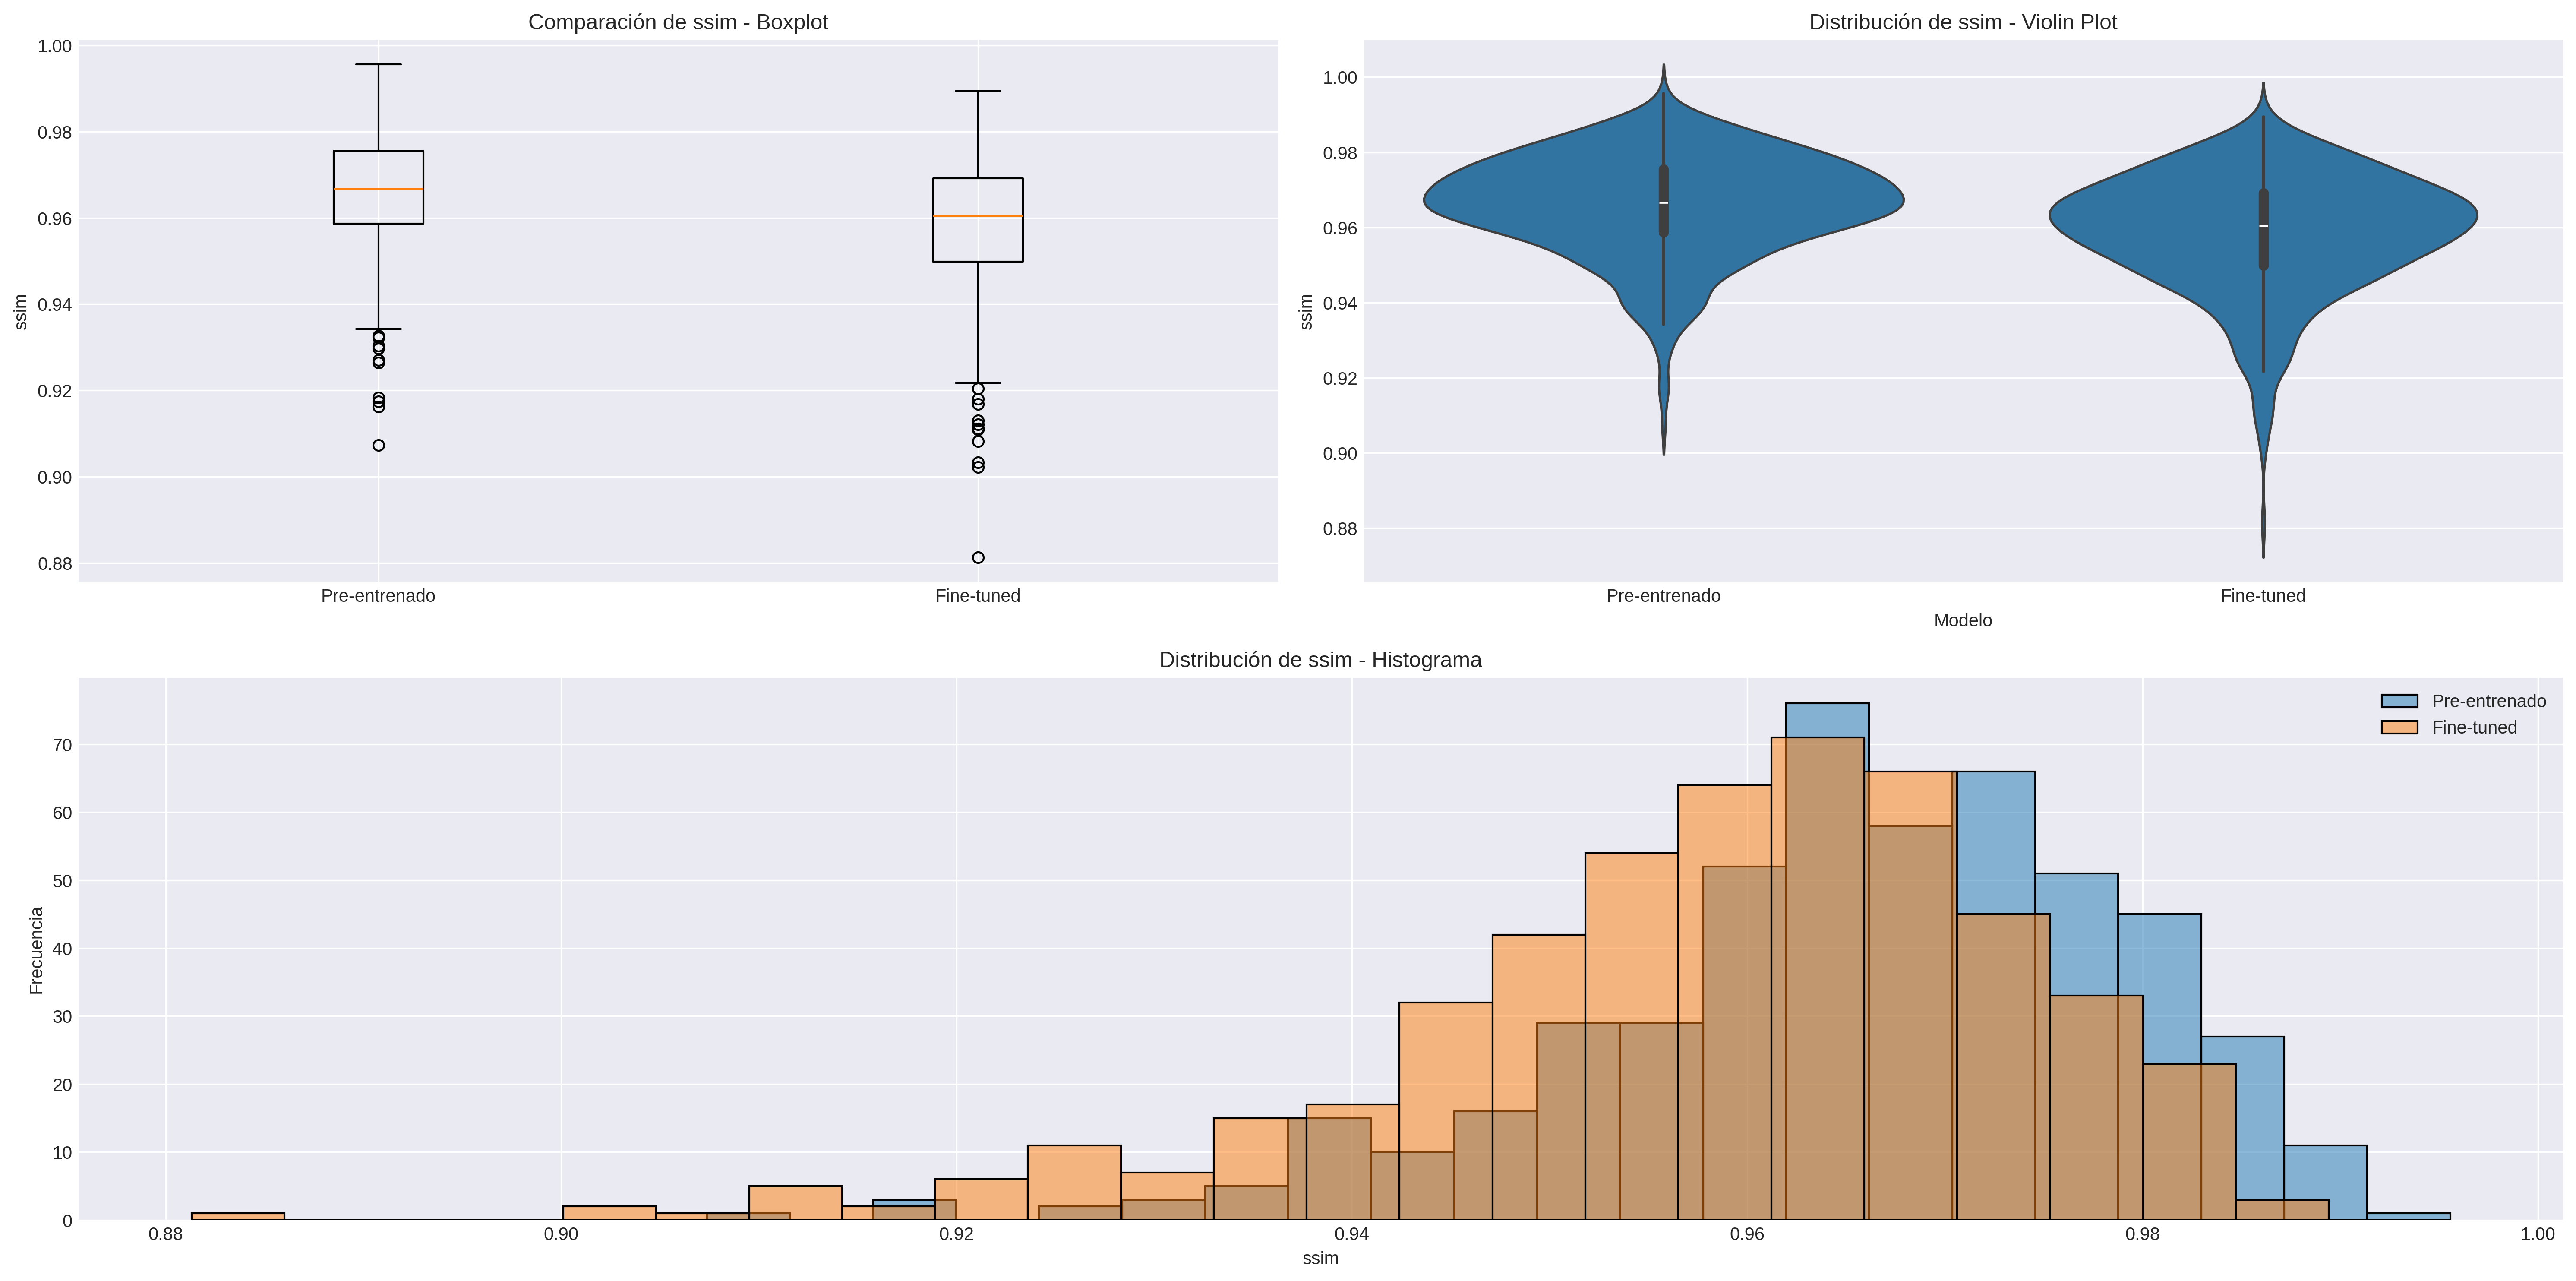
\includegraphics[width=\textwidth]{Images/comparison_plots_ssim_no_phy.png}
        \caption{Comparación entre fine-tuning sin componente física y modelo pre-entrenado}
        \label{fig:ssim_hist}
    \end{subfigure}
    \hfill
    \begin{subfigure}[b]{0.48\textwidth}
        \centering
        % FT No-Structural vs Baseline
        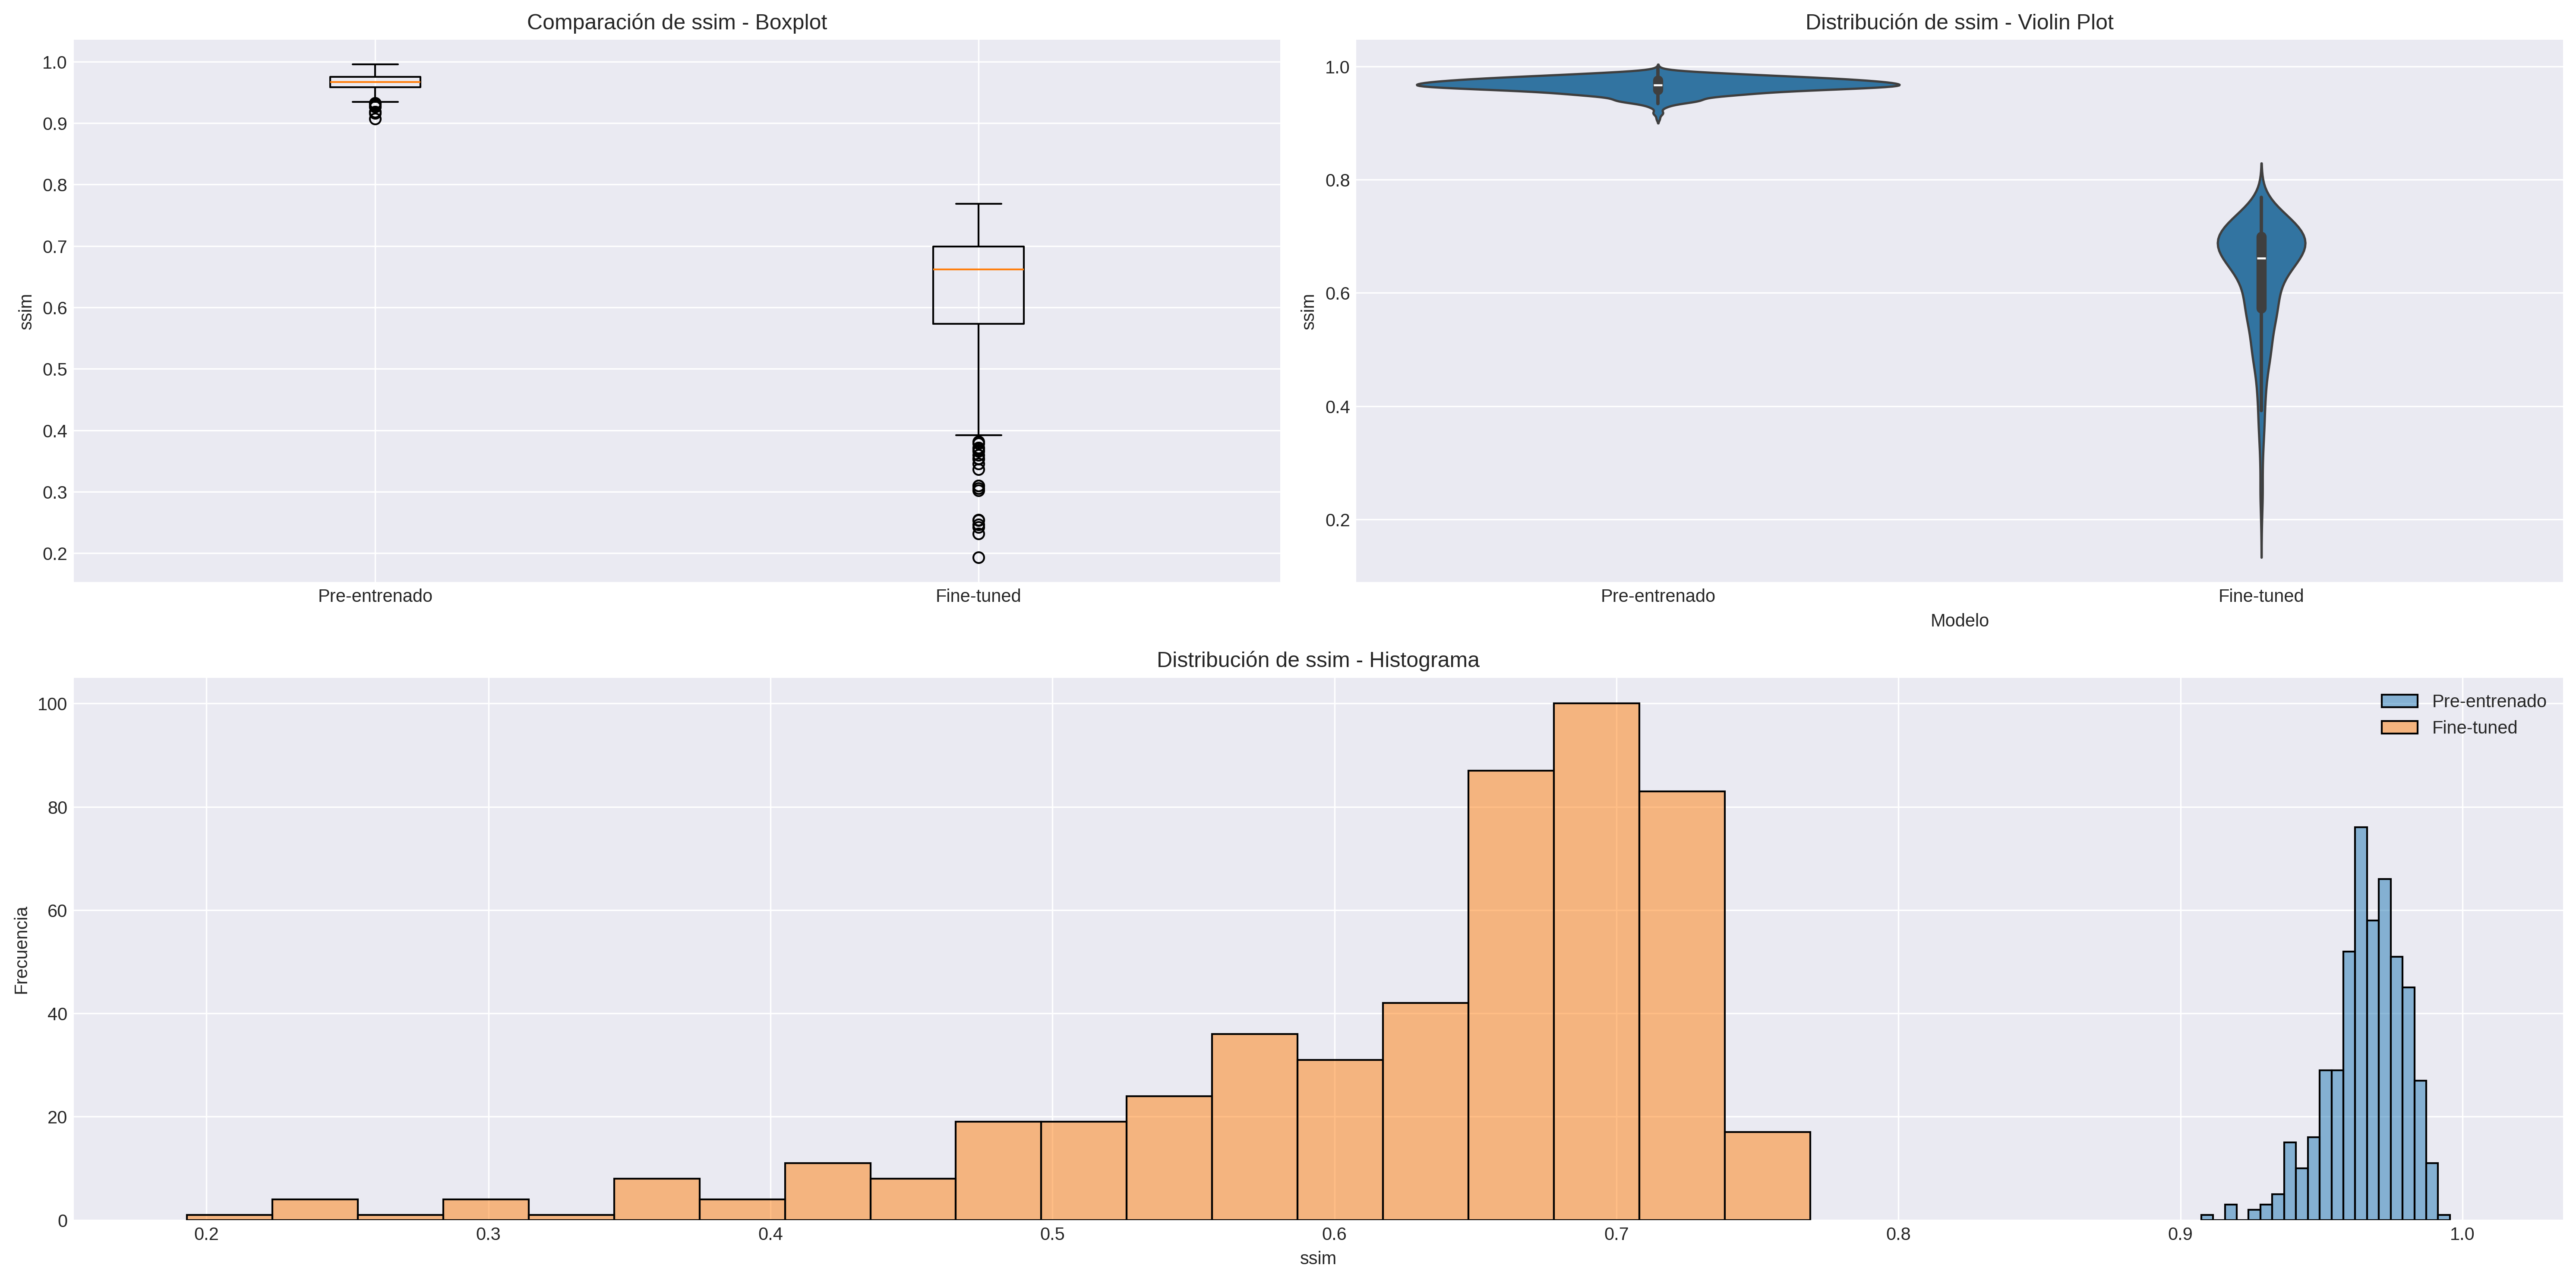
\includegraphics[width=\textwidth]{Images/comparison_plots_ssim_no_struct.png}
        \caption{Comparación entre fine-tuning sin componente estructural y modelo pre-entrenado}
        \label{fig:ssim_violin}
    \end{subfigure}
    
    \vspace{0.5cm}
    
    \begin{subfigure}[b]{0.7\textwidth}
        \centering
        % FT vs Baseline
        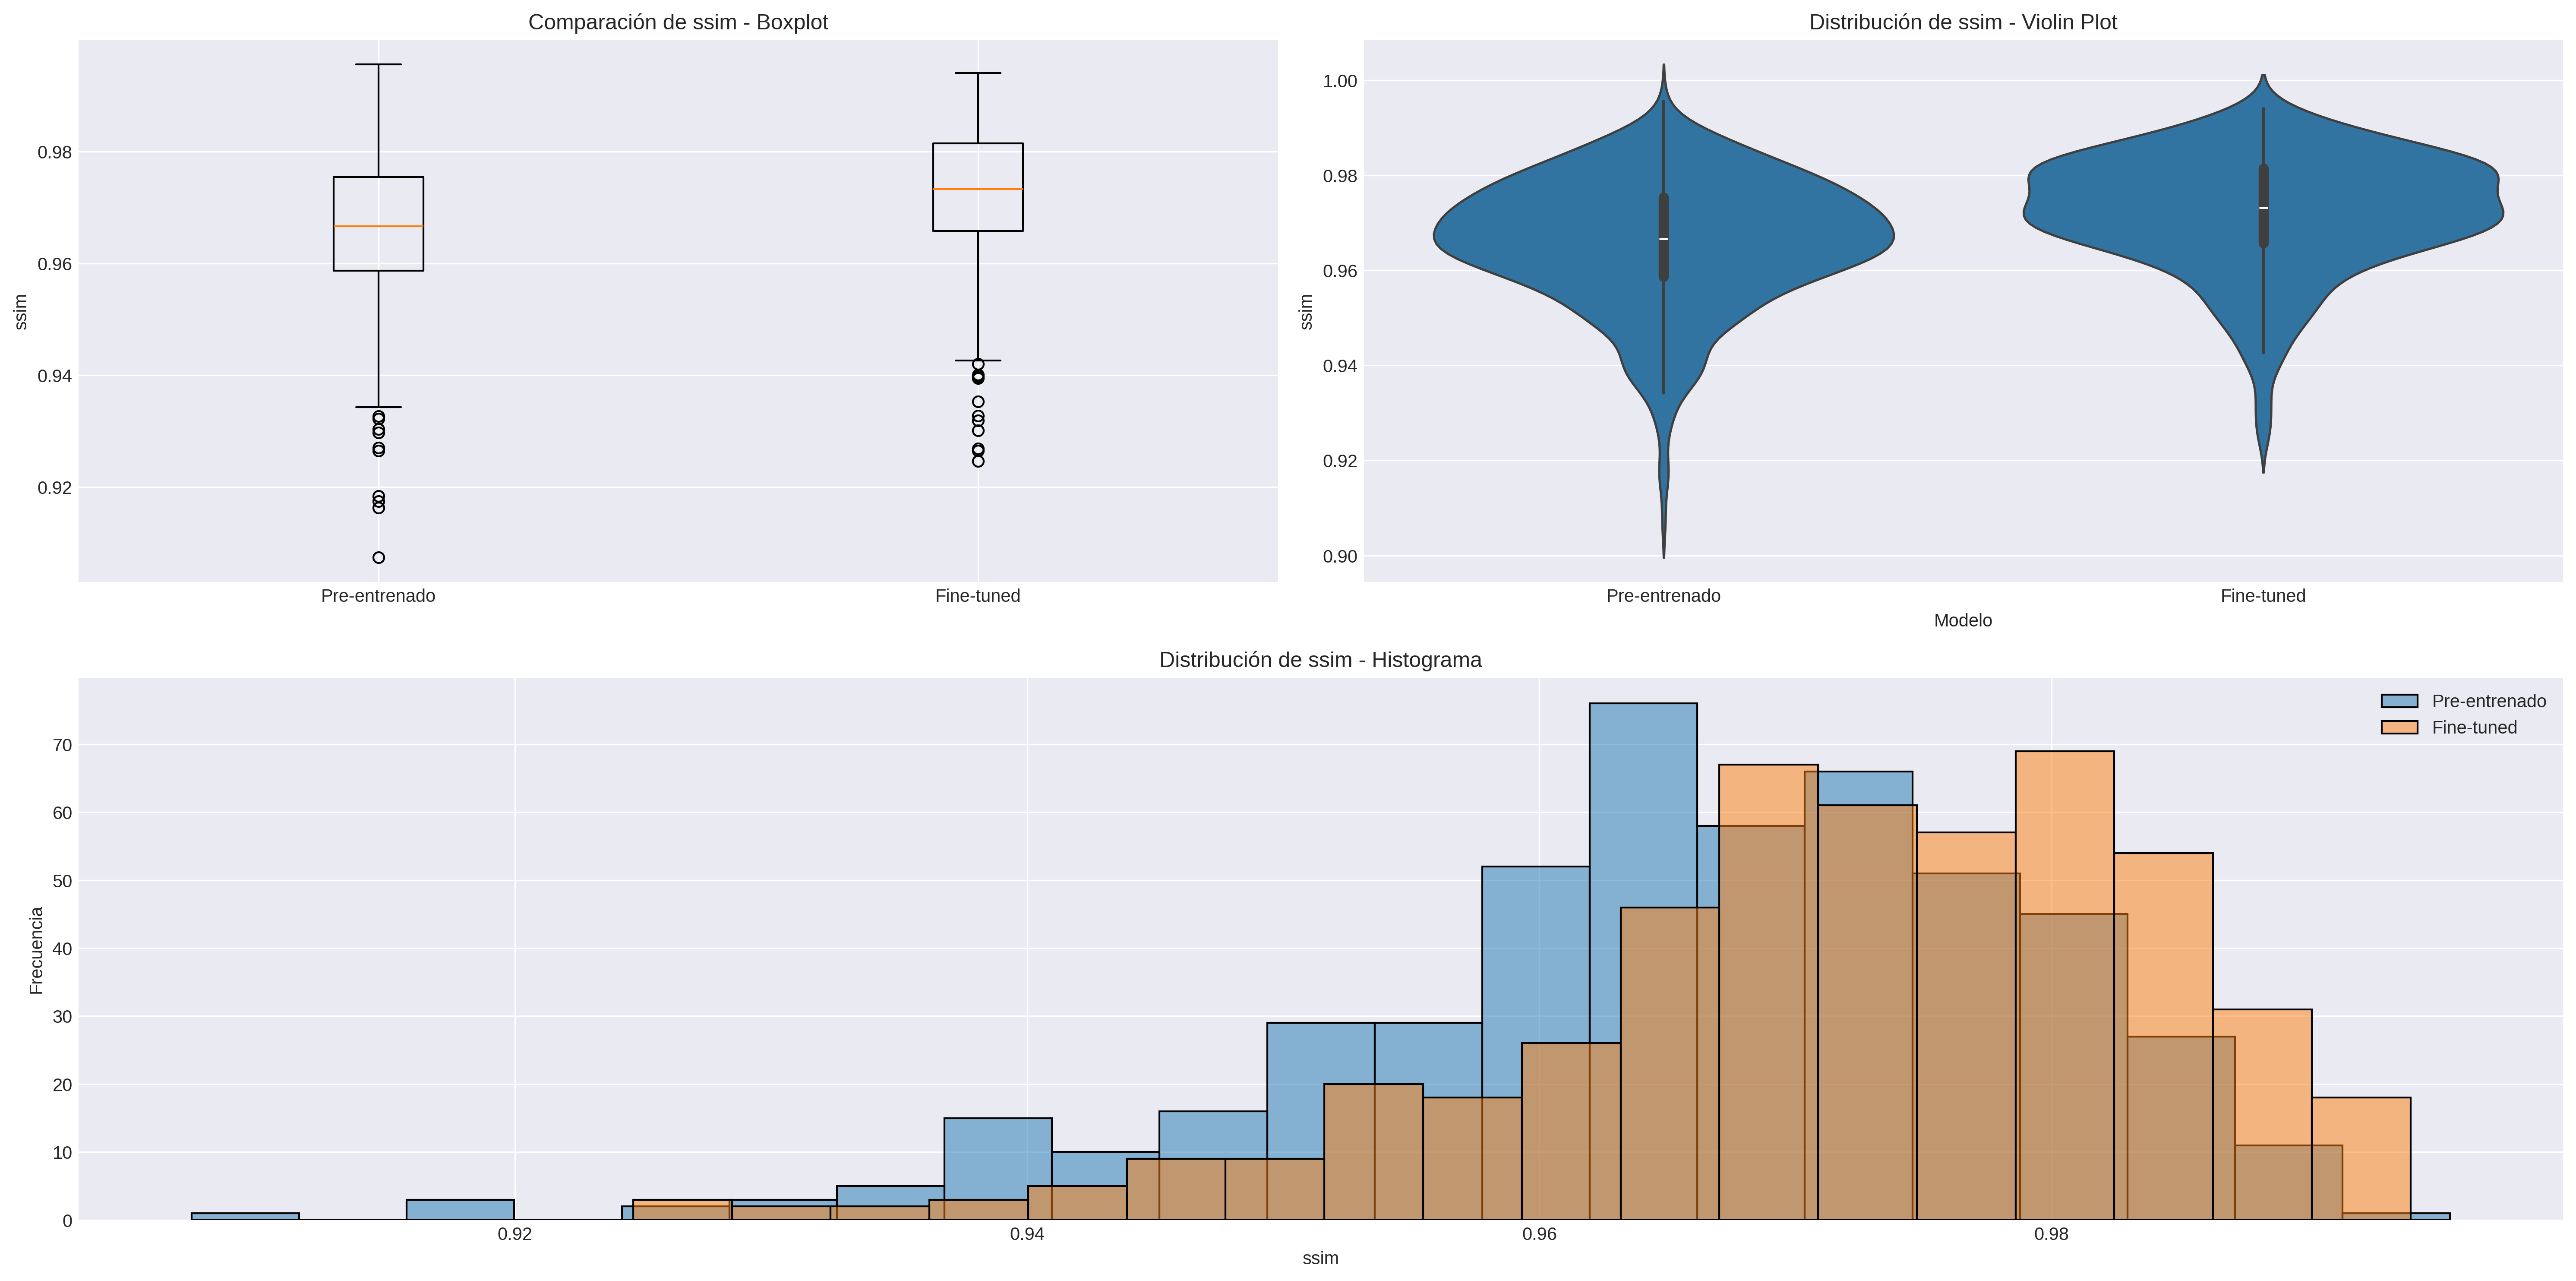
\includegraphics[width=\textwidth]{Images/comparison_plots_ssim_sup.png}
        \caption{Comparación entre fine-tuning (FT) completo y modelo pre-entrenado}
        \label{fig:ssim_box}
    \end{subfigure}
    
    \caption{Análisis comparativo del Índice de Similitud Estructural (SSIM) entre el modelo pre-entrenado y las variantes de fine-tuning implementadas. a) Comparación entre fine-tuning sin componente física y modelo pre-entrenado. b) Comparación entre fine-tuning sin componente estructural y modelo pre-entrenado. c) Comparación entre fine-tuning completo y modelo pre-entrenado.}
    \label{fig:ssim_analysis}
\end{figure}


\paragraph{Fine-tuning Completo (FT)}
El modelo con fine-tuning completo logra una mejora significativa en la calidad perceptual de las reconstrucciones. El SSIM medio aumentó de 0.9658 en el modelo pre-entrenado a 0.9721 en el modelo fine-tuned, lo que representa una mejora en la similitud estructural. Aunque este incremento pueda parecer modesto en términos absolutos, es importante contextualizar que estos valores ya están muy cerca del máximo teórico de 1.0, lo que hace que cualquier mejora en este rango sea particularmente significativa.

La calidad y consistencia de las reconstrucciones se refleja en varios aspectos:

\begin{itemize}
    \item La mediana mejoró de 0.9666 a 0.9732, indicando una mejora sistemática en la tendencia central
    \item La variabilidad se redujo, con una disminución en la desviación estándar de 0.0135 a 0.0123
    \item El valor mínimo aumentó de 0.9074 a 0.9246, sugiriendo una mejor capacidad para manejar casos difíciles
    \item El valor máximo se mantuvo muy alto, cercano a 0.99 en ambos casos
\end{itemize}

El análisis estadístico confirma la significancia de estas mejoras:

\begin{itemize}
    \item La prueba t pareada $(t = -18.8183, p < 0.001)$ y la prueba de Wilcoxon $(W = 14074.0000, p < 0.001)$ demuestran que la mejora es estadísticamente significativa
    \item El tamaño del efecto $(d$ de $Cohen = -0.4819)$ indica un impacto positivo de magnitud media a grande
    \item Las pruebas de Shapiro-Wilk revelan desviaciones de la normalidad en ambas distribuciones, subrayando la importancia de las pruebas no paramétricas
\end{itemize}

\paragraph{Fine-tuning sin Componente Física (FT No-Physical)}
La eliminación de la componente física resulta en una degradación leve pero significativa de la calidad estructural. El SSIM medio disminuyó a 0.9583, representando una pérdida relativamente pequeña pero estadísticamente significativa. Este resultado sugiere que la componente física, aunque importante, no es crítica para mantener la similitud estructural básica entre las imágenes originales y reconstruidas.

Los cambios en la distribución del SSIM son sutiles pero notables:

\begin{itemize}
    \item La mediana descendió levemente a 0.9605
    \item Se observó un ligero aumento en la variabilidad (desviación estándar de 0.0157)
    \item El valor mínimo disminuyó a 0.8813, indicando una mayor dificultad con casos desafiantes
\end{itemize}

Las pruebas estadísticas confirman la significancia de estos cambios:

\begin{itemize}
    \item El estadístico $t$ de $25.0947$ ($p < 0.001$) y el estadístico de Wilcoxon $W = 3218.0000$ ($p < 0.001$) indican diferencias significativas
    \item El tamaño del efecto ($d$ de $Cohen = 0.5123$) sugiere un impacto negativo substancial
\end{itemize}

\paragraph{Fine-tuning sin Componente Estructural (FT No-Structural)}
La ausencia de la componente estructural produce un deterioro dramático en la calidad perceptual de las reconstrucciones. El SSIM medio cayó significativamente a 0.6257, representando una degradación masiva en la similitud estructural. Esta caída de más de 0.34 puntos es particularmente alarmante dado que el SSIM es una métrica que típicamente muestra cambios más sutiles.

El impacto devastador se manifiesta en múltiples aspectos:

\begin{itemize}
    \item Una caída dramática en el valor máximo a 0.7688, muy por debajo del rango típico de calidad aceptable
    \item Un valor mínimo extremadamente bajo de 0.1930, indicando casos de reconstrucción muy deficiente
    \item Un aumento masivo en la variabilidad (desviación estándar de 0.1041), sugiriendo una pérdida de consistencia en la calidad de reconstrucción
\end{itemize}

El análisis estadístico revela la magnitud sin precedentes de este deterioro:

\begin{itemize}
    \item La prueba t pareada muestra un efecto extremadamente fuerte ($t = 76.6244$, $p < 0.001$)
    \item La prueba de Wilcoxon ($W = 0.0000$, $p < 0.001$) confirma la uniformidad del deterioro
    \item El tamaño del efecto ($d$ de $Cohen = 4.5827$) indica un impacto negativo excepcionalmente grande
\end{itemize}

Este análisis del SSIM proporciona una perspectiva crucial centrada en la calidad perceptual de las reconstrucciones. Los resultados demuestran de manera contundente que la componente estructural es absolutamente esencial para mantener la fidelidad visual de las reconstrucciones, mientras que la componente física juega un papel más sutil pero significativo. La caída dramática en el SSIM al eliminar la componente estructural sugiere que esta pérdida no solo afecta métricas numéricas sino que también tiene un impacto sustancial en la calidad visual percibida de las reconstrucciones.

\subsection{Predicciones}

En esta sección, se presentan los resultados de las predicciones realizadas por el modelo pre-entrenado y los modelos fine-tuned en el conjunto de datos de validación. Las predicciones se comparan con los valores reales para evaluar la capacidad de los modelos para generalizar a datos no vistos. Se analizan las distribuciones de los errores de predicción y se realizan pruebas estadísticas para evaluar la significancia de las diferencias entre los modelos.


\begin{figure}[H]
    \centering
    \begin{subfigure}[b]{0.8\textwidth}
        \centering
        % Baseline 
        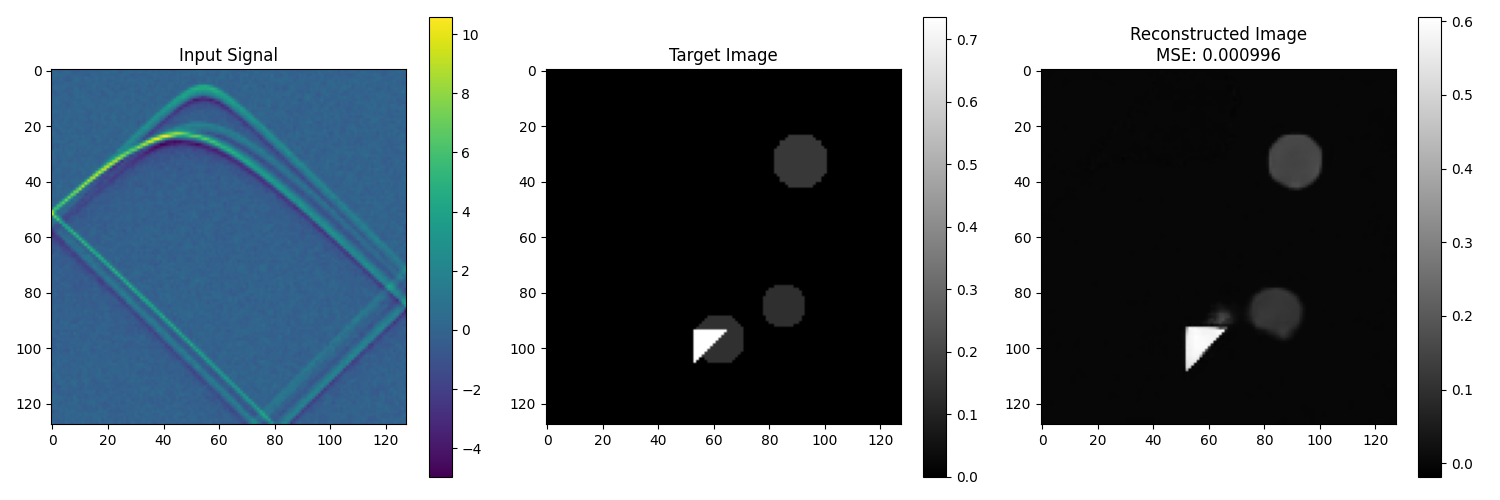
\includegraphics[width=\textwidth]{Images/sample_solo.png}
        \caption{Ejemplo de predicciones realizadas por el modelo pre-entrenado.}
        \label{fig:sample_solo}
    \end{subfigure}

    \vspace{0.5cm}
    
    \begin{subfigure}[b]{0.8\textwidth}
        \centering
        % FT (Full)
        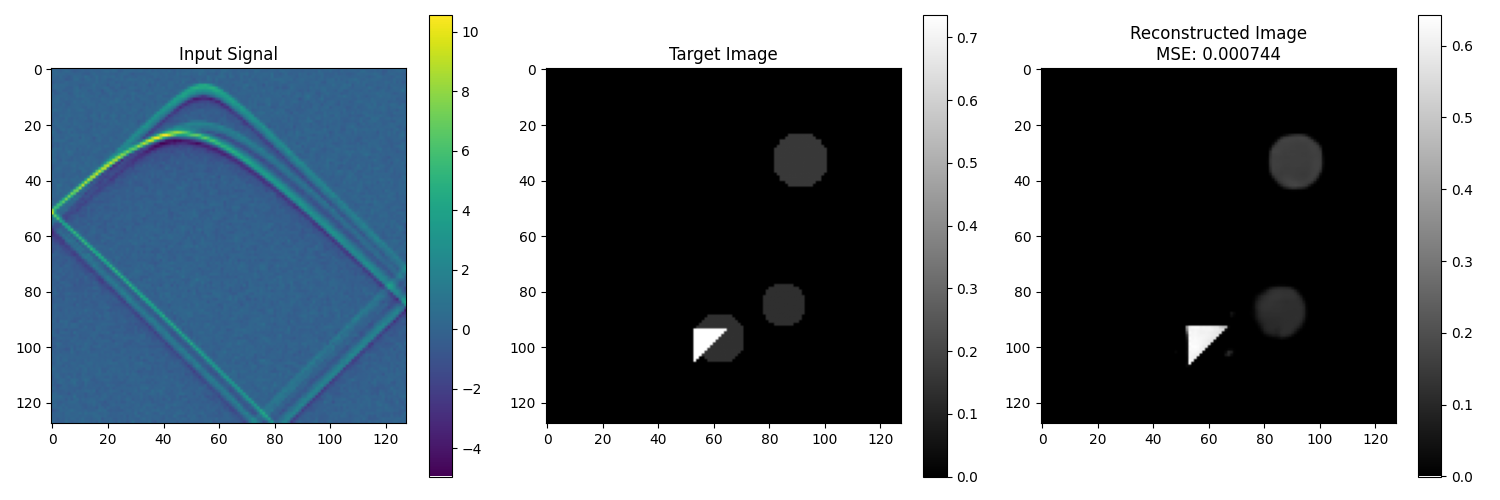
\includegraphics[width=\textwidth]{Images/sample_sup.png}
        \caption{Ejemplo de predicciones realizadas por el modelo fine-tuned completo.}
        \label{fig:sample_sup}
    \end{subfigure}
    
    \vspace{0.5cm}
    
    \begin{subfigure}[b]{0.8\textwidth}
        \centering
        % FT (No-Structural)
        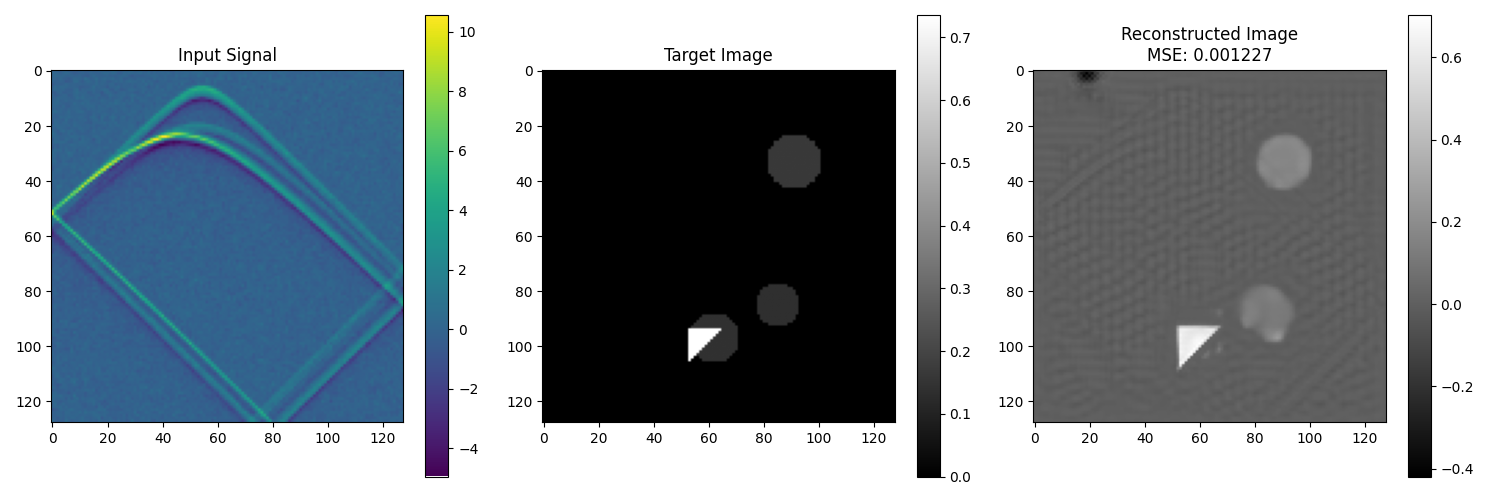
\includegraphics[width=\textwidth]{Images/sample_no_struct.png}
        \caption{Ejemplo de predicciones realizadas por el modelo fine-tuned sin componente estructural.}
        \label{fig:sample_no_struct}
    \end{subfigure}
    
    \begin{subfigure}[b]{0.8\textwidth}
        \centering
        % FT (No-Physical)
        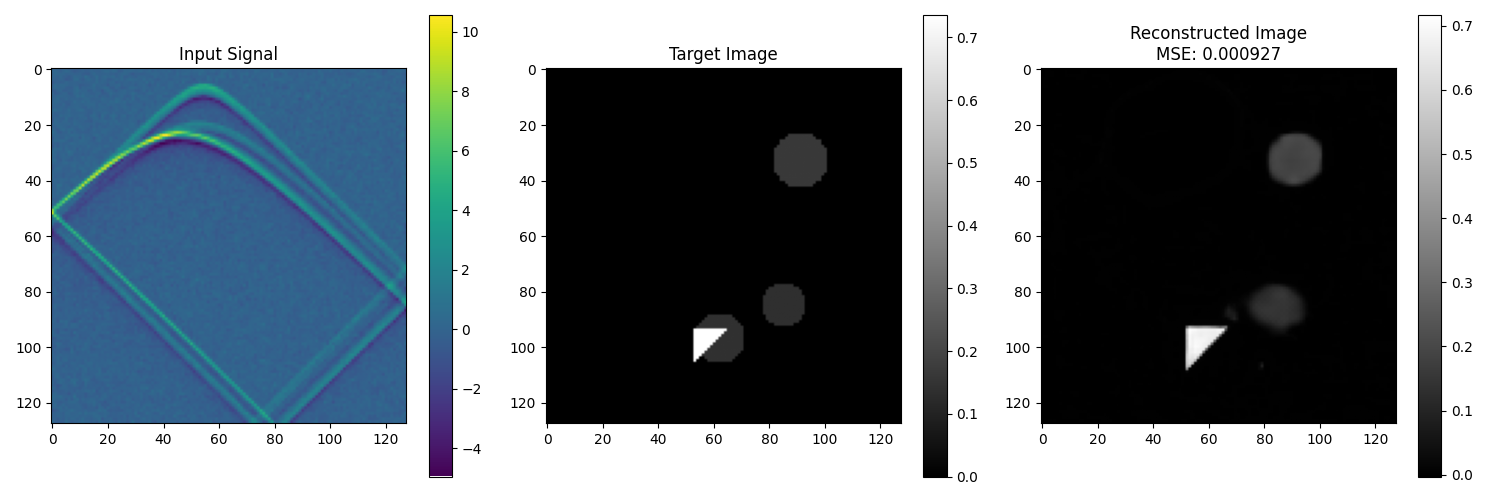
\includegraphics[width=\textwidth]{Images/sample_no_phy.png}
        \caption{Ejemplo de predicciones realizadas por el modelo fine-tuned sin componente física.}
        \label{fig:sample_no_phy}
    \end{subfigure}

    \caption{Ejemplos de predicciones realizadas por el modelo pre-entrenado y los modelos fine-tuned en el conjunto de datos de validación.}
    \label{fig:sample_analysis}
\end{figure}





%%%%% -------- Analysis -------- %%%%%
\maincontent{Análisis y Discusión} % Modificado para incluir discusión
\input{6_Analysis}

%%%%% ------ Conclusion ------ %%%%%
\maincontent{Conclusiones y Trabajo Futuro}
\sectionisblank

%%%%% ------ Appendices ------ %%%%% % Añadido apéndices
\appendix
\maincontent{Apéndices}
\input{8_Appendices}

%%%%% ------ References ------ %%%%%
\backmatter{Referencias}
\bibliographystyle{abbrv}
\bibliography{references}

% Ensure all citations are defined
\nocite{*}

\end{document}